% ***************************************************
% A Classic Thesis Style
% An Homage to The Elements of Typographic Style
%
% Copyright (C) 2012 Andr\'e Miede http://www.miede.de
%
% If you like the style then I would appreciate a postcard. My
% address can be found in the file ClassicThesis.pdf. A collection
% of the postcards I received so far is available online at 
% http://postcards.miede.de
%
% License:
% This program is free software; you can redistribute it and/or
% modify it under the terms of the GNU General Public License as
% published by the Free Software Foundation; either version 2 of
% the License, or (at your option) any later version.
%
% This program is distributed in the hope that it will be useful,
% but WITHOUT ANY WARRANTY; without even the implied warranty of
% MERCHANTABILITY or FITNESS FOR A PARTICULAR PURPOSE.  See the
% GNU General Public License for more details.
%
% You should have received a copy of the GNU General Public
% License along with this program; see the file COPYING.  If not,
% write to the Free Software Foundation, Inc., 59 Temple Place -
% Suite 330, Boston, MA 02111-1307, USA.
%
% ***************************************************************
% Note:
%    * You must not use "u etc. in strings/commands that will be
%      spaced out (use \"u or real umlauts instead)
%    * New enumeration (small caps): \begin{aenumerate}
%      \end{aenumerate}
% 	 * For margin notes: \marginpar or \graffito{}
%    * Do not use bold fonts in this style, it is designed around
%      them
%    * Use tables as in the examples
%    * See classicthesis-preamble.sty for useful commands
% ****************************************************************

\documentclass[ twoside,  %rende lo stampato fronte-retro
				%oneside,  %rendere lo stampato solo fronte
				openright,
				% letterpaper a4paper
				titlepage, 
				numbers=noenddot,
				headinclude, %1headlines
				footinclude=true, 
				cleardoublepage=empty,
				%abstractoff, % <--- obsolete, remove (todo)
				BCOR=5mm,
				paper=a4, 
				fontsize=12pt, %11pt,in origine
				]{scrreprt}

%*****************************************************************
% Note: Make all your adjustments in here
%*****************************************************************
\usepackage{algorithm}
\usepackage{algpseudocode}
\usepackage{xspace}
\algnewcommand{\algorithmicgoto}{\textbf{go to}}%
\algnewcommand{\Goto}{\algorithmicgoto\xspace}%
\algnewcommand{\Label}{\Statex\unskip}

\usepackage{mwe}
%\usepackage{subcaption}

\usepackage[backref, backend=biber]{biblatex}
\bibliography{Bibliography}	




% ****************************************************************
% classicthesis-config.tex 
% formerly known as loadpackages.sty, classicthesis-ldpkg.sty, and
% classicthesis-preamble.sty Use it at the beginning of your
% ClassicThesis.tex, or as a LaTeX Preamble in your
% ClassicThesis.{tex,lyx} with % ****************************************************************
% classicthesis-config.tex 
% formerly known as loadpackages.sty, classicthesis-ldpkg.sty, and
% classicthesis-preamble.sty Use it at the beginning of your
% ClassicThesis.tex, or as a LaTeX Preamble in your
% ClassicThesis.{tex,lyx} with % ****************************************************************
% classicthesis-config.tex 
% formerly known as loadpackages.sty, classicthesis-ldpkg.sty, and
% classicthesis-preamble.sty Use it at the beginning of your
% ClassicThesis.tex, or as a LaTeX Preamble in your
% ClassicThesis.{tex,lyx} with \input{classicthesis-config}
% ****************************************************************
% If you like the classicthesis, then I would appreciate a
% postcard. My address can be found in the file
% ClassicThesis.pdf. A collection of the postcards I received so
% far is available online at http://postcards.miede.de
% ****************************************************************

% ****************************************************************
% 1. Configure classicthesis for your needs here, e.g., remove
% "drafting" below in order to deactivate the time-stamp on the
% pages
% ****************************************************************
\PassOptionsToPackage{eulerchapternumbers,
						listings,
						%drafting,
						pdfspacing,
						floatperchapter,
						%linedheaders,
						subfig,
						beramono,
						eulermath,
						parts}{classicthesis}										

% ****************************************************************
% Triggers for this config
% **************************************************************** 
\usepackage{ifthen}
\newboolean{enable-backrefs} % enable backrefs in the bibliography
\setboolean{enable-backrefs}{false} % true false
% TODO backref is incompatible?
% ****************************************************************


% ****************************************************************
% 2. Personal data and user ad-hoc commands
% ****************************************************************
\newcommand{\myTitleIT}{Bluetooth Low Energy e Risparmio Energetico \xspace}
\newcommand{\myFirstAuthorName}{Lorenzo Pagliari\xspace}
\newcommand{\myMatrFirstAuthor}{798273\xspace}
\newcommand{\mySupervisor}{Prof.Raffaela Mirandola\xspace} % relatore
\newcommand{\myOtherSupervisor}{Diego Carmelo Perez Palacin\xspace} % co relatori
%\newcommand{\myFaculty}{Facolt\`a di Ingegneria\xspace}
\newcommand{\mySchool}{Scuola di Ingegneria Industriale e dell'Informazione\xspace}
\newcommand{\myDepartment}{Dipartimento di Elettronica, Informazione e Bioingegneria\xspace}
\newcommand{\myCourseFirstPartIT}{Corso di Laurea Magistrale in\xspace}
\newcommand{\myCourseSecondPartIT}{Ingegneria Informatica\xspace}
\newcommand{\myUni}{Politecnico di Milano\xspace}
\newcommand{\myLocation}{Milano\xspace}
\newcommand{\myTime}{Settembre 2015\xspace}
\newcommand{\myVersion}{version 1.0\xspace}
\newcommand{\myAcademicYear}{Anno Accademico 2014-2015\xspace}

% ********************************************************************
% Setup, fine tuning, and useful commands
% ********************************************************************
\newcounter{dummy} % necessary for correct hyperlinks (to index, bib, etc.)
\newlength{\abcd} % for ab..z string length calculation
\providecommand{\mLyX}{L\kern-.1667em\lower.25em\hbox{Y}\kern-.125emX\@}
% from here till the end of the section, you can modify whatever you want
\newcommand{\ie}{i.\,e.\ }
\newcommand{\Ie}{I.\,e.\ }
\newcommand{\eg}{e.\,g.\ }
\newcommand{\Eg}{E.\,g.\ }
% referencing commands
\newcommand{\myEq}[1]{equazione \eqref{#1}}
\newcommand{\MyEq}[1]{Equazione \eqref{#1}}
\newcommand{\myFig}[1]{figura \ref{#1}}
\newcommand{\MyFig}[1]{Figura \ref{#1}}
\newcommand{\myTab}[1]{tabella \ref{#1}}
\newcommand{\MyTab}[1]{Tabella \ref{#1}}
\newcommand{\mySubsec}[1]{sottosezione\ref{#1}}
\newcommand{\MySubsec}[1]{Sottosezione \ref{#1}}
\newcommand{\mySec}[1]{sezione \ref{#1}}
\newcommand{\MySec}[1]{Sezione \ref{#1}}
\newcommand{\myChap}[1]{capitolo \ref{#1}}
\newcommand{\MyChap}[1]{Capitolo \ref{#1}}
\newcommand{\myAppendix}[1]{appendice \ref{#1}}
\newcommand{\MyAppendix}[1]{Appendice \ref{#1}}
\newcommand{\myEmph}[1]{\textsc{#1}}

% **********************************************************************


% **********************************************************************
% 3. Loading some handy packages
% **********************************************************************
\PassOptionsToPackage{T1}{fontenc} % T2A for cyrillics
\usepackage{fontenc} 
\PassOptionsToPackage{utf8}{inputenc} % latin9 (ISO-8859-9) = latin1+"Euro sign"
\usepackage{inputenc}				

\PassOptionsToPackage{autostyle,italian=guillemets,threshold=2}{csquotes}
\usepackage{csquotes}

\PassOptionsToPackage{american,italian}{babel}
\usepackage{babel}

\PassOptionsToPackage{fleqn}{amsmath} % math environments and more by the AMS 
\usepackage{amsmath}

\usepackage{amsthm}
\theoremstyle{definition}

\newtheorem{definition}{Definition}

\usepackage{textcomp} % fix warning with missing font shapes
\usepackage{scrhack} % fix warnings when using KOMA with listings package          
\usepackage{xspace} % to get the spacing after macros right  
\usepackage{mparhack} % get marginpar right
\usepackage{fixltx2e} % fixes some LaTeX stuff 

\PassOptionsToPackage{printonlyused,smaller}{acronym}
\usepackage{acronym} % nice macros for handling all acronyms in the thesis
% **********************************************************************


% **********************************************************************
% 4. Setup floats: tables, (sub)figures, and captions
% **********************************************************************
\usepackage{tabularx} % better tables
\setlength{\extrarowheight}{3pt} % increase table row height
\newcommand{\tableheadline}[2]{\multicolumn{1}{#1}{\normalsize\spacedlowsmallcaps{#2}}}
\newcommand{\tableheadlineMore}[3]{\multicolumn{#1}{#2}{\normalsize\spacedlowsmallcaps{#3}}}
\newcommand{\tablefirstcol}[2]{\multicolumn{1}{#1}{\textbf{#2}}}

\usepackage{caption}
\captionsetup{format=hang,labelfont={sf,bf},font=small}
\usepackage{colortbl}
\usepackage{multirow}

\usepackage{subfig}
\usepackage{siunitx}
% *********************************************************************


% *********************************************************************
% 5. Setup code listings
% *********************************************************************
\usepackage{listings}
\lstloadlanguages{bash, C++, Java, Matlab}

% for special keywords
\lstset{language=[LaTeX]Tex,
	keywordstyle=\color{RoyalBlue},%\bfseries,
	basicstyle=\small\ttfamily,
	%identifierstyle=\color{NavyBlue},
	commentstyle=\color{Green}\ttfamily,
	stringstyle=\rmfamily,
	numbers=none,%left,%
	numberstyle=\scriptsize,%\tiny
	stepnumber=5,
	numbersep=8pt,
	showstringspaces=false,
	breaklines=true,
	frameround=ftff,
	frame=single,
	belowcaptionskip=.75\baselineskip
	%frame=L
} 
% *********************************************************************


% *********************************************************************
% 6. PDFLaTeX, hyperreferences and citation backreferences
% *********************************************************************
% ********************************************************************
% Using PDFLaTeX
% ********************************************************************
\PassOptionsToPackage{pdftex,hyperfootnotes=false,pdfpagelabels}{hyperref}
\usepackage{hyperref}  % backref linktocpage pagebackref
\pdfcompresslevel=9
\pdfadjustspacing=1 
\PassOptionsToPackage{pdftex}{graphicx}
\usepackage{graphicx} 

% ********************************************************************
% Setup the style of the backrefs from the bibliography
% (translate the options to any language you use)
% ********************************************************************
\newcommand{\backrefnotcitedstring}{\relax}%(Not cited.)
\newcommand{\backrefcitedsinglestring}[1]{(Cited on page~#1.)}
\newcommand{\backrefcitedmultistring}[1]{(Cited on pages~#1.)}
\ifthenelse{\boolean{enable-backrefs}}%
{%
	\PassOptionsToPackage{hyperpageref}{backref}
	\usepackage{backref} % to be loaded after hyperref package 
	\renewcommand{\backreftwosep}{ and~} % separate 2 pages
	\renewcommand{\backreflastsep}{, and~} % separate last of longer list
	\renewcommand*{\backref}[1]{}  % disable standard
	\renewcommand*{\backrefalt}[4]{% detailed backref
		\ifcase #1 %
		\backrefnotcitedstring%
		\or%
		\backrefcitedsinglestring{#2}%
		\else%
		\backrefcitedmultistring{#2}%
		\fi}%
}{\relax}    


% ****************************************************************
% PDF/A compliance
% ****************************************************************
% TODO not working: requires downloading color specification file in a specific
% tex folder and other hacks I don't want to spend time with
% \usepackage[a-1b]{pdfx}

% ********************************************************************
% Hyperreferences
% ********************************************************************
\hypersetup{%
	%draft,	% = no hyperlinking at all (useful in b/w printouts)
	colorlinks=true, linktocpage=true, pdfstartpage=3, pdfstartview=FitV,%
	% uncomment the following line if you want to have black links (e.g., for printing)
	%colorlinks=false, linktocpage=false, pdfborder={0 0 0}, pdfstartpage=3, pdfstartview=FitV,% 
	breaklinks=true, pdfpagemode=UseNone, pageanchor=true, pdfpagemode=UseOutlines,%
	plainpages=false, bookmarksnumbered, bookmarksopen=true, bookmarksopenlevel=1,%
	hypertexnames=true, pdfhighlight=/O,%nesting=true,%frenchlinks,%
	urlcolor=webbrown, linkcolor=RoyalBlue, citecolor=webgreen, %pagecolor=RoyalBlue,%
	%urlcolor=Black, linkcolor=Black, citecolor=Black, %pagecolor=Black,%
} 

%pdftitle={\myTitle},%
%pdfauthor={\textcopyright\ \myFirstAuthorName and \mySecondAuthorName, \myUni, \myFaculty},%
%pdfsubject={},%
%pdfkeywords={},%
%pdfcreator={pdfLaTeX},%
%pdfproducer={LaTeX with hyperref and classicthesis}%

%}   

% ********************************************************************
% Setup autoreferences
% ********************************************************************
% There are some issues regarding autorefnames
% http://www.ureader.de/msg/136221647.aspx
% http://www.tex.ac.uk/cgi-bin/texfaq2html?label=latexwords
% you have to redefine the makros for the 
% language you use, e.g., american, ngerman
% (as chosen when loading babel/AtBeginDocument)
% ********************************************************************
\makeatletter
\@ifpackageloaded{babel}%
{%
	\addto\extrasamerican{%
		\renewcommand*{\figureautorefname}{Figure}%
		\renewcommand*{\tableautorefname}{Table}%
		\renewcommand*{\partautorefname}{Part}%
		\renewcommand*{\chapterautorefname}{Chapter}%
		\renewcommand*{\sectionautorefname}{Section}%
		\renewcommand*{\subsectionautorefname}{Section}%
		\renewcommand*{\subsubsectionautorefname}{Section}% 	
	}%
	\addto\extrasitalian{% 
		\renewcommand*{\paragraphautorefname}{Paragrafo}%
		\renewcommand*{\subparagraphautorefname}{Paragrafo}%
		\renewcommand*{\footnoteautorefname}{Nota a pié di pagina}%
		\renewcommand*{\FancyVerbLineautorefname}{Zeile}%
		\renewcommand*{\theoremautorefname}{Teorema}%
		\renewcommand*{\appendixautorefname}{Appendice}%
		\renewcommand*{\equationautorefname}{Equazione}%        
		\renewcommand*{\itemautorefname}{Punto}%
	}%	
	% Fix to getting autorefs for subfigures right (thanks to Belinda Vogt for changing the definition)
	\providecommand{\subfigureautorefname}{\figureautorefname}%  			
}{\relax}
\makeatother

% ****************************************************************
% 7. Last calls before the bar closes
% ****************************************************************

\usepackage{classicthesis} 

% ****************************************************************
% ****************************************************************
% If you like the classicthesis, then I would appreciate a
% postcard. My address can be found in the file
% ClassicThesis.pdf. A collection of the postcards I received so
% far is available online at http://postcards.miede.de
% ****************************************************************

% ****************************************************************
% 1. Configure classicthesis for your needs here, e.g., remove
% "drafting" below in order to deactivate the time-stamp on the
% pages
% ****************************************************************
\PassOptionsToPackage{eulerchapternumbers,
						listings,
						%drafting,
						pdfspacing,
						floatperchapter,
						%linedheaders,
						subfig,
						beramono,
						eulermath,
						parts}{classicthesis}										

% ****************************************************************
% Triggers for this config
% **************************************************************** 
\usepackage{ifthen}
\newboolean{enable-backrefs} % enable backrefs in the bibliography
\setboolean{enable-backrefs}{false} % true false
% TODO backref is incompatible?
% ****************************************************************


% ****************************************************************
% 2. Personal data and user ad-hoc commands
% ****************************************************************
\newcommand{\myTitleIT}{Bluetooth Low Energy e Risparmio Energetico \xspace}
\newcommand{\myFirstAuthorName}{Lorenzo Pagliari\xspace}
\newcommand{\myMatrFirstAuthor}{798273\xspace}
\newcommand{\mySupervisor}{Prof.Raffaela Mirandola\xspace} % relatore
\newcommand{\myOtherSupervisor}{Diego Carmelo Perez Palacin\xspace} % co relatori
%\newcommand{\myFaculty}{Facolt\`a di Ingegneria\xspace}
\newcommand{\mySchool}{Scuola di Ingegneria Industriale e dell'Informazione\xspace}
\newcommand{\myDepartment}{Dipartimento di Elettronica, Informazione e Bioingegneria\xspace}
\newcommand{\myCourseFirstPartIT}{Corso di Laurea Magistrale in\xspace}
\newcommand{\myCourseSecondPartIT}{Ingegneria Informatica\xspace}
\newcommand{\myUni}{Politecnico di Milano\xspace}
\newcommand{\myLocation}{Milano\xspace}
\newcommand{\myTime}{Settembre 2015\xspace}
\newcommand{\myVersion}{version 1.0\xspace}
\newcommand{\myAcademicYear}{Anno Accademico 2014-2015\xspace}

% ********************************************************************
% Setup, fine tuning, and useful commands
% ********************************************************************
\newcounter{dummy} % necessary for correct hyperlinks (to index, bib, etc.)
\newlength{\abcd} % for ab..z string length calculation
\providecommand{\mLyX}{L\kern-.1667em\lower.25em\hbox{Y}\kern-.125emX\@}
% from here till the end of the section, you can modify whatever you want
\newcommand{\ie}{i.\,e.\ }
\newcommand{\Ie}{I.\,e.\ }
\newcommand{\eg}{e.\,g.\ }
\newcommand{\Eg}{E.\,g.\ }
% referencing commands
\newcommand{\myEq}[1]{equazione \eqref{#1}}
\newcommand{\MyEq}[1]{Equazione \eqref{#1}}
\newcommand{\myFig}[1]{figura \ref{#1}}
\newcommand{\MyFig}[1]{Figura \ref{#1}}
\newcommand{\myTab}[1]{tabella \ref{#1}}
\newcommand{\MyTab}[1]{Tabella \ref{#1}}
\newcommand{\mySubsec}[1]{sottosezione\ref{#1}}
\newcommand{\MySubsec}[1]{Sottosezione \ref{#1}}
\newcommand{\mySec}[1]{sezione \ref{#1}}
\newcommand{\MySec}[1]{Sezione \ref{#1}}
\newcommand{\myChap}[1]{capitolo \ref{#1}}
\newcommand{\MyChap}[1]{Capitolo \ref{#1}}
\newcommand{\myAppendix}[1]{appendice \ref{#1}}
\newcommand{\MyAppendix}[1]{Appendice \ref{#1}}
\newcommand{\myEmph}[1]{\textsc{#1}}

% **********************************************************************


% **********************************************************************
% 3. Loading some handy packages
% **********************************************************************
\PassOptionsToPackage{T1}{fontenc} % T2A for cyrillics
\usepackage{fontenc} 
\PassOptionsToPackage{utf8}{inputenc} % latin9 (ISO-8859-9) = latin1+"Euro sign"
\usepackage{inputenc}				

\PassOptionsToPackage{autostyle,italian=guillemets,threshold=2}{csquotes}
\usepackage{csquotes}

\PassOptionsToPackage{american,italian}{babel}
\usepackage{babel}

\PassOptionsToPackage{fleqn}{amsmath} % math environments and more by the AMS 
\usepackage{amsmath}

\usepackage{amsthm}
\theoremstyle{definition}

\newtheorem{definition}{Definition}

\usepackage{textcomp} % fix warning with missing font shapes
\usepackage{scrhack} % fix warnings when using KOMA with listings package          
\usepackage{xspace} % to get the spacing after macros right  
\usepackage{mparhack} % get marginpar right
\usepackage{fixltx2e} % fixes some LaTeX stuff 

\PassOptionsToPackage{printonlyused,smaller}{acronym}
\usepackage{acronym} % nice macros for handling all acronyms in the thesis
% **********************************************************************


% **********************************************************************
% 4. Setup floats: tables, (sub)figures, and captions
% **********************************************************************
\usepackage{tabularx} % better tables
\setlength{\extrarowheight}{3pt} % increase table row height
\newcommand{\tableheadline}[2]{\multicolumn{1}{#1}{\normalsize\spacedlowsmallcaps{#2}}}
\newcommand{\tableheadlineMore}[3]{\multicolumn{#1}{#2}{\normalsize\spacedlowsmallcaps{#3}}}
\newcommand{\tablefirstcol}[2]{\multicolumn{1}{#1}{\textbf{#2}}}

\usepackage{caption}
\captionsetup{format=hang,labelfont={sf,bf},font=small}
\usepackage{colortbl}
\usepackage{multirow}

\usepackage{subfig}
\usepackage{siunitx}
% *********************************************************************


% *********************************************************************
% 5. Setup code listings
% *********************************************************************
\usepackage{listings}
\lstloadlanguages{bash, C++, Java, Matlab}

% for special keywords
\lstset{language=[LaTeX]Tex,
	keywordstyle=\color{RoyalBlue},%\bfseries,
	basicstyle=\small\ttfamily,
	%identifierstyle=\color{NavyBlue},
	commentstyle=\color{Green}\ttfamily,
	stringstyle=\rmfamily,
	numbers=none,%left,%
	numberstyle=\scriptsize,%\tiny
	stepnumber=5,
	numbersep=8pt,
	showstringspaces=false,
	breaklines=true,
	frameround=ftff,
	frame=single,
	belowcaptionskip=.75\baselineskip
	%frame=L
} 
% *********************************************************************


% *********************************************************************
% 6. PDFLaTeX, hyperreferences and citation backreferences
% *********************************************************************
% ********************************************************************
% Using PDFLaTeX
% ********************************************************************
\PassOptionsToPackage{pdftex,hyperfootnotes=false,pdfpagelabels}{hyperref}
\usepackage{hyperref}  % backref linktocpage pagebackref
\pdfcompresslevel=9
\pdfadjustspacing=1 
\PassOptionsToPackage{pdftex}{graphicx}
\usepackage{graphicx} 

% ********************************************************************
% Setup the style of the backrefs from the bibliography
% (translate the options to any language you use)
% ********************************************************************
\newcommand{\backrefnotcitedstring}{\relax}%(Not cited.)
\newcommand{\backrefcitedsinglestring}[1]{(Cited on page~#1.)}
\newcommand{\backrefcitedmultistring}[1]{(Cited on pages~#1.)}
\ifthenelse{\boolean{enable-backrefs}}%
{%
	\PassOptionsToPackage{hyperpageref}{backref}
	\usepackage{backref} % to be loaded after hyperref package 
	\renewcommand{\backreftwosep}{ and~} % separate 2 pages
	\renewcommand{\backreflastsep}{, and~} % separate last of longer list
	\renewcommand*{\backref}[1]{}  % disable standard
	\renewcommand*{\backrefalt}[4]{% detailed backref
		\ifcase #1 %
		\backrefnotcitedstring%
		\or%
		\backrefcitedsinglestring{#2}%
		\else%
		\backrefcitedmultistring{#2}%
		\fi}%
}{\relax}    


% ****************************************************************
% PDF/A compliance
% ****************************************************************
% TODO not working: requires downloading color specification file in a specific
% tex folder and other hacks I don't want to spend time with
% \usepackage[a-1b]{pdfx}

% ********************************************************************
% Hyperreferences
% ********************************************************************
\hypersetup{%
	%draft,	% = no hyperlinking at all (useful in b/w printouts)
	colorlinks=true, linktocpage=true, pdfstartpage=3, pdfstartview=FitV,%
	% uncomment the following line if you want to have black links (e.g., for printing)
	%colorlinks=false, linktocpage=false, pdfborder={0 0 0}, pdfstartpage=3, pdfstartview=FitV,% 
	breaklinks=true, pdfpagemode=UseNone, pageanchor=true, pdfpagemode=UseOutlines,%
	plainpages=false, bookmarksnumbered, bookmarksopen=true, bookmarksopenlevel=1,%
	hypertexnames=true, pdfhighlight=/O,%nesting=true,%frenchlinks,%
	urlcolor=webbrown, linkcolor=RoyalBlue, citecolor=webgreen, %pagecolor=RoyalBlue,%
	%urlcolor=Black, linkcolor=Black, citecolor=Black, %pagecolor=Black,%
} 

%pdftitle={\myTitle},%
%pdfauthor={\textcopyright\ \myFirstAuthorName and \mySecondAuthorName, \myUni, \myFaculty},%
%pdfsubject={},%
%pdfkeywords={},%
%pdfcreator={pdfLaTeX},%
%pdfproducer={LaTeX with hyperref and classicthesis}%

%}   

% ********************************************************************
% Setup autoreferences
% ********************************************************************
% There are some issues regarding autorefnames
% http://www.ureader.de/msg/136221647.aspx
% http://www.tex.ac.uk/cgi-bin/texfaq2html?label=latexwords
% you have to redefine the makros for the 
% language you use, e.g., american, ngerman
% (as chosen when loading babel/AtBeginDocument)
% ********************************************************************
\makeatletter
\@ifpackageloaded{babel}%
{%
	\addto\extrasamerican{%
		\renewcommand*{\figureautorefname}{Figure}%
		\renewcommand*{\tableautorefname}{Table}%
		\renewcommand*{\partautorefname}{Part}%
		\renewcommand*{\chapterautorefname}{Chapter}%
		\renewcommand*{\sectionautorefname}{Section}%
		\renewcommand*{\subsectionautorefname}{Section}%
		\renewcommand*{\subsubsectionautorefname}{Section}% 	
	}%
	\addto\extrasitalian{% 
		\renewcommand*{\paragraphautorefname}{Paragrafo}%
		\renewcommand*{\subparagraphautorefname}{Paragrafo}%
		\renewcommand*{\footnoteautorefname}{Nota a pié di pagina}%
		\renewcommand*{\FancyVerbLineautorefname}{Zeile}%
		\renewcommand*{\theoremautorefname}{Teorema}%
		\renewcommand*{\appendixautorefname}{Appendice}%
		\renewcommand*{\equationautorefname}{Equazione}%        
		\renewcommand*{\itemautorefname}{Punto}%
	}%	
	% Fix to getting autorefs for subfigures right (thanks to Belinda Vogt for changing the definition)
	\providecommand{\subfigureautorefname}{\figureautorefname}%  			
}{\relax}
\makeatother

% ****************************************************************
% 7. Last calls before the bar closes
% ****************************************************************

\usepackage{classicthesis} 

% ****************************************************************
% ****************************************************************
% If you like the classicthesis, then I would appreciate a
% postcard. My address can be found in the file
% ClassicThesis.pdf. A collection of the postcards I received so
% far is available online at http://postcards.miede.de
% ****************************************************************

% ****************************************************************
% 1. Configure classicthesis for your needs here, e.g., remove
% "drafting" below in order to deactivate the time-stamp on the
% pages
% ****************************************************************
\PassOptionsToPackage{eulerchapternumbers,
						listings,
						%drafting,
						pdfspacing,
						floatperchapter,
						%linedheaders,
						subfig,
						beramono,
						eulermath,
						parts}{classicthesis}										

% ****************************************************************
% Triggers for this config
% **************************************************************** 
\usepackage{ifthen}
\newboolean{enable-backrefs} % enable backrefs in the bibliography
\setboolean{enable-backrefs}{false} % true false
% TODO backref is incompatible?
% ****************************************************************


% ****************************************************************
% 2. Personal data and user ad-hoc commands
% ****************************************************************
\newcommand{\myTitleIT}{Bluetooth Low Energy e Risparmio Energetico \xspace}
\newcommand{\myFirstAuthorName}{Lorenzo Pagliari\xspace}
\newcommand{\myMatrFirstAuthor}{798273\xspace}
\newcommand{\mySupervisor}{Prof.Raffaela Mirandola\xspace} % relatore
\newcommand{\myOtherSupervisor}{Diego Carmelo Perez Palacin\xspace} % co relatori
%\newcommand{\myFaculty}{Facolt\`a di Ingegneria\xspace}
\newcommand{\mySchool}{Scuola di Ingegneria Industriale e dell'Informazione\xspace}
\newcommand{\myDepartment}{Dipartimento di Elettronica, Informazione e Bioingegneria\xspace}
\newcommand{\myCourseFirstPartIT}{Corso di Laurea Magistrale in\xspace}
\newcommand{\myCourseSecondPartIT}{Ingegneria Informatica\xspace}
\newcommand{\myUni}{Politecnico di Milano\xspace}
\newcommand{\myLocation}{Milano\xspace}
\newcommand{\myTime}{Settembre 2015\xspace}
\newcommand{\myVersion}{version 1.0\xspace}
\newcommand{\myAcademicYear}{Anno Accademico 2014-2015\xspace}

% ********************************************************************
% Setup, fine tuning, and useful commands
% ********************************************************************
\newcounter{dummy} % necessary for correct hyperlinks (to index, bib, etc.)
\newlength{\abcd} % for ab..z string length calculation
\providecommand{\mLyX}{L\kern-.1667em\lower.25em\hbox{Y}\kern-.125emX\@}
% from here till the end of the section, you can modify whatever you want
\newcommand{\ie}{i.\,e.\ }
\newcommand{\Ie}{I.\,e.\ }
\newcommand{\eg}{e.\,g.\ }
\newcommand{\Eg}{E.\,g.\ }
% referencing commands
\newcommand{\myEq}[1]{equazione \eqref{#1}}
\newcommand{\MyEq}[1]{Equazione \eqref{#1}}
\newcommand{\myFig}[1]{figura \ref{#1}}
\newcommand{\MyFig}[1]{Figura \ref{#1}}
\newcommand{\myTab}[1]{tabella \ref{#1}}
\newcommand{\MyTab}[1]{Tabella \ref{#1}}
\newcommand{\mySubsec}[1]{sottosezione\ref{#1}}
\newcommand{\MySubsec}[1]{Sottosezione \ref{#1}}
\newcommand{\mySec}[1]{sezione \ref{#1}}
\newcommand{\MySec}[1]{Sezione \ref{#1}}
\newcommand{\myChap}[1]{capitolo \ref{#1}}
\newcommand{\MyChap}[1]{Capitolo \ref{#1}}
\newcommand{\myAppendix}[1]{appendice \ref{#1}}
\newcommand{\MyAppendix}[1]{Appendice \ref{#1}}
\newcommand{\myEmph}[1]{\textsc{#1}}

% **********************************************************************


% **********************************************************************
% 3. Loading some handy packages
% **********************************************************************
\PassOptionsToPackage{T1}{fontenc} % T2A for cyrillics
\usepackage{fontenc} 
\PassOptionsToPackage{utf8}{inputenc} % latin9 (ISO-8859-9) = latin1+"Euro sign"
\usepackage{inputenc}				

\PassOptionsToPackage{autostyle,italian=guillemets,threshold=2}{csquotes}
\usepackage{csquotes}

\PassOptionsToPackage{american,italian}{babel}
\usepackage{babel}

\PassOptionsToPackage{fleqn}{amsmath} % math environments and more by the AMS 
\usepackage{amsmath}

\usepackage{amsthm}
\theoremstyle{definition}

\newtheorem{definition}{Definition}

\usepackage{textcomp} % fix warning with missing font shapes
\usepackage{scrhack} % fix warnings when using KOMA with listings package          
\usepackage{xspace} % to get the spacing after macros right  
\usepackage{mparhack} % get marginpar right
\usepackage{fixltx2e} % fixes some LaTeX stuff 

\PassOptionsToPackage{printonlyused,smaller}{acronym}
\usepackage{acronym} % nice macros for handling all acronyms in the thesis
% **********************************************************************


% **********************************************************************
% 4. Setup floats: tables, (sub)figures, and captions
% **********************************************************************
\usepackage{tabularx} % better tables
\setlength{\extrarowheight}{3pt} % increase table row height
\newcommand{\tableheadline}[2]{\multicolumn{1}{#1}{\normalsize\spacedlowsmallcaps{#2}}}
\newcommand{\tableheadlineMore}[3]{\multicolumn{#1}{#2}{\normalsize\spacedlowsmallcaps{#3}}}
\newcommand{\tablefirstcol}[2]{\multicolumn{1}{#1}{\textbf{#2}}}

\usepackage{caption}
\captionsetup{format=hang,labelfont={sf,bf},font=small}
\usepackage{colortbl}
\usepackage{multirow}

\usepackage{subfig}
\usepackage{siunitx}
% *********************************************************************


% *********************************************************************
% 5. Setup code listings
% *********************************************************************
\usepackage{listings}
\lstloadlanguages{bash, C++, Java, Matlab}

% for special keywords
\lstset{language=[LaTeX]Tex,
	keywordstyle=\color{RoyalBlue},%\bfseries,
	basicstyle=\small\ttfamily,
	%identifierstyle=\color{NavyBlue},
	commentstyle=\color{Green}\ttfamily,
	stringstyle=\rmfamily,
	numbers=none,%left,%
	numberstyle=\scriptsize,%\tiny
	stepnumber=5,
	numbersep=8pt,
	showstringspaces=false,
	breaklines=true,
	frameround=ftff,
	frame=single,
	belowcaptionskip=.75\baselineskip
	%frame=L
} 
% *********************************************************************


% *********************************************************************
% 6. PDFLaTeX, hyperreferences and citation backreferences
% *********************************************************************
% ********************************************************************
% Using PDFLaTeX
% ********************************************************************
\PassOptionsToPackage{pdftex,hyperfootnotes=false,pdfpagelabels}{hyperref}
\usepackage{hyperref}  % backref linktocpage pagebackref
\pdfcompresslevel=9
\pdfadjustspacing=1 
\PassOptionsToPackage{pdftex}{graphicx}
\usepackage{graphicx} 

% ********************************************************************
% Setup the style of the backrefs from the bibliography
% (translate the options to any language you use)
% ********************************************************************
\newcommand{\backrefnotcitedstring}{\relax}%(Not cited.)
\newcommand{\backrefcitedsinglestring}[1]{(Cited on page~#1.)}
\newcommand{\backrefcitedmultistring}[1]{(Cited on pages~#1.)}
\ifthenelse{\boolean{enable-backrefs}}%
{%
	\PassOptionsToPackage{hyperpageref}{backref}
	\usepackage{backref} % to be loaded after hyperref package 
	\renewcommand{\backreftwosep}{ and~} % separate 2 pages
	\renewcommand{\backreflastsep}{, and~} % separate last of longer list
	\renewcommand*{\backref}[1]{}  % disable standard
	\renewcommand*{\backrefalt}[4]{% detailed backref
		\ifcase #1 %
		\backrefnotcitedstring%
		\or%
		\backrefcitedsinglestring{#2}%
		\else%
		\backrefcitedmultistring{#2}%
		\fi}%
}{\relax}    


% ****************************************************************
% PDF/A compliance
% ****************************************************************
% TODO not working: requires downloading color specification file in a specific
% tex folder and other hacks I don't want to spend time with
% \usepackage[a-1b]{pdfx}

% ********************************************************************
% Hyperreferences
% ********************************************************************
\hypersetup{%
	%draft,	% = no hyperlinking at all (useful in b/w printouts)
	colorlinks=true, linktocpage=true, pdfstartpage=3, pdfstartview=FitV,%
	% uncomment the following line if you want to have black links (e.g., for printing)
	%colorlinks=false, linktocpage=false, pdfborder={0 0 0}, pdfstartpage=3, pdfstartview=FitV,% 
	breaklinks=true, pdfpagemode=UseNone, pageanchor=true, pdfpagemode=UseOutlines,%
	plainpages=false, bookmarksnumbered, bookmarksopen=true, bookmarksopenlevel=1,%
	hypertexnames=true, pdfhighlight=/O,%nesting=true,%frenchlinks,%
	urlcolor=webbrown, linkcolor=RoyalBlue, citecolor=webgreen, %pagecolor=RoyalBlue,%
	%urlcolor=Black, linkcolor=Black, citecolor=Black, %pagecolor=Black,%
} 

%pdftitle={\myTitle},%
%pdfauthor={\textcopyright\ \myFirstAuthorName and \mySecondAuthorName, \myUni, \myFaculty},%
%pdfsubject={},%
%pdfkeywords={},%
%pdfcreator={pdfLaTeX},%
%pdfproducer={LaTeX with hyperref and classicthesis}%

%}   

% ********************************************************************
% Setup autoreferences
% ********************************************************************
% There are some issues regarding autorefnames
% http://www.ureader.de/msg/136221647.aspx
% http://www.tex.ac.uk/cgi-bin/texfaq2html?label=latexwords
% you have to redefine the makros for the 
% language you use, e.g., american, ngerman
% (as chosen when loading babel/AtBeginDocument)
% ********************************************************************
\makeatletter
\@ifpackageloaded{babel}%
{%
	\addto\extrasamerican{%
		\renewcommand*{\figureautorefname}{Figure}%
		\renewcommand*{\tableautorefname}{Table}%
		\renewcommand*{\partautorefname}{Part}%
		\renewcommand*{\chapterautorefname}{Chapter}%
		\renewcommand*{\sectionautorefname}{Section}%
		\renewcommand*{\subsectionautorefname}{Section}%
		\renewcommand*{\subsubsectionautorefname}{Section}% 	
	}%
	\addto\extrasitalian{% 
		\renewcommand*{\paragraphautorefname}{Paragrafo}%
		\renewcommand*{\subparagraphautorefname}{Paragrafo}%
		\renewcommand*{\footnoteautorefname}{Nota a pié di pagina}%
		\renewcommand*{\FancyVerbLineautorefname}{Zeile}%
		\renewcommand*{\theoremautorefname}{Teorema}%
		\renewcommand*{\appendixautorefname}{Appendice}%
		\renewcommand*{\equationautorefname}{Equazione}%        
		\renewcommand*{\itemautorefname}{Punto}%
	}%	
	% Fix to getting autorefs for subfigures right (thanks to Belinda Vogt for changing the definition)
	\providecommand{\subfigureautorefname}{\figureautorefname}%  			
}{\relax}
\makeatother

% ****************************************************************
% 7. Last calls before the bar closes
% ****************************************************************

\usepackage{classicthesis} 

% ****************************************************************

%*****************************************************************
% Hyphenation
%*****************************************************************
\hyphenation{put-here-the-words-latex-cannot-hyphenate}

\begin{document}
	
	% initial, local settings
	\numberwithin{equation}{chapter}
	\frenchspacing
	\raggedbottom
	\selectlanguage{italian} % american/italian
	\pagenumbering{roman}
	\pagestyle{plain}
	
	%*************************************************************
	% Frontmatter
	%*************************************************************
	
	% Uncomment the following line to add the ''copertina'' to the pdf
	%%*******************************************************
%
%			COPERTINA
%
%
%*******************************************************
\begin{titlepage}
	% if you want the titlepage to be centered, uncomment and fine-tune the line below (KOMA classes environment)
	\begin{addmargin}[-1cm]{-3cm}
	\begin{center}
		%\large %nse si usa 11pt
		\spacedlowsmallcaps{\myUni} \\
		\bigskip\myFaculty \\
		\medskip\mySchool \\
		\medskip\myDepartment \\
		\bigskip\myCourseFirstPartIT \\
		\medskip\myCourseSecondPartIT \\  
		
		\hfill
		
		\vfill
		
		\begin{figure}[!h]
			\begin{addmargin}[-1cm]{-3cm}
				\centering
				\includegraphics[width=0.3\columnwidth]{\myLogo} % or \logo.eps on windows 
			\end{addmargin}
		\end{figure}
		
		\vfill
		
		\begingroup
		%\huge %se si usa 11pt
		\LARGE %se si usa 12pt
		\color{Maroon} \myTitleIT \\ \bigskip
		\endgroup
		
		\vfill
		
		\flushleft 
		%\normalsize{Relatore:}\\ %se si usa 11pt
		\small{Relatore:}\\ %se si usa 12pt
		\medskip\spacedlowsmallcaps{\mySupervisor}
		
		\flushleft
		%\normalsize{Correlatore:}\\ %se si usa 11pt
		\small{Correlatore:}\\ %se si usa 12pt
		\medskip\spacedlowsmallcaps{\myOtherSupervisor}\\
		%comment if there isn't any other supervisor
		%\flushleft
		%\normalsize{Correlatore Alta Scuola Politecnica:}\\
		%\medskip\spacedlowsmallcaps{\myOtherOtherSupervisor}\\
		
		\vfill  
		
		\flushright
		%\normalsize{Tesi di Laurea Magistrale di:}\\ %se si usa 11pt
		\small{Tesi di Laurea Magistrale di:}\\ %se si usa 12pt
		\medskip \spacedlowsmallcaps{\myFirstAuthorName}\\
		Matricola n. \myMatrFirstAuthor \\ 
		
		\vfill 
		
		\centering {\myAcademicYear}                     
		
	\end{center}
	\end{addmargin}
\end{titlepage} %è un frontespizio centrato
	
	%*******************************************************
% Titlepage
%   the file is named in italian since our language 
%   provide different words for different things and
%   we should use them
%*******************************************************
\begin{titlepage}
	% if you want the titlepage to be centered, uncomment and fine-tune the line below (KOMA classes environment)
	% \begin{addmargin}[-1cm]{-3cm}
    \begin{center}
    	\large
        \spacedlowsmallcaps{\myUni} \\
        \bigskip
        %\myFaculty \\
        \medskip\mySchool \\
    	\medskip\myDepartment \\
    	\bigskip\myCourseFirstPartIT \\
        \medskip\myCourseSecondPartIT \\  

        \hfill

        \vfill
        
        \begin{figure}[!h]
			\begin{center}
				
\includegraphics[width=0.3\columnwidth]{Images/logoPoli.pdf} % or \logo.eps on windows 
			\end{center}
		\end{figure}
		
		\vfill

        \begingroup
       		\huge	
            \color{Maroon} \myTitleIT \\ \bigskip
        \endgroup

        \vfill

		\flushleft 
		\normalsize{Relatore:}\\
		\medskip\spacedlowsmallcaps{\mySupervisor}

		\flushleft
		\normalsize{Correlatore:}\\
		\medskip\spacedlowsmallcaps{\myOtherSupervisor}\\
		%comment if there isn't any other supervisor
		%\flushleft
		%\normalsize{Correlatore Alta Scuola Politecnica:}\\
		%\medskip\spacedlowsmallcaps{\myOtherOtherSupervisor}\\
        
        \vfill  
        
        \flushright
        \normalsize{Tesi di Laurea Magistrale di:}\\
        \medskip \spacedlowsmallcaps{\myFirstAuthorName}\\
		Matricola n. \myMatrFirstAuthor \\ 
				
		\vfill 

		\centering {\myAcademicYear}                     

    \end{center}  
  %\end{addmargin}       
\end{titlepage}
	
	\thispagestyle{empty}

\hfill

\vfill

\pdfbookmark[0]{Colophon}{colophon}
\section*{Colophon}
This document was typeset using the typographical look-and-feel
\texttt{classicthesis} developed by Andr\'e Miede.
The style was inspired by Robert Bringhurst's seminal book on
typography ``\emph{The Elements of Typographic Style}''.
\texttt{classicthesis} is available for both \LaTeX\ and \mLyX: 
\begin{center}
\url{http://code.google.com/p/classicthesis/}
\end{center}
Happy users of \texttt{classicthesis} usually send a real postcard
to the author, a collection of postcards received so far is
featured here:
\begin{center}
\url{http://postcards.miede.de/}
\end{center}
 
\bigskip

\noindent\myFirstAuthorName:
\textit{\myTitleIT},
\myTime

\medskip

%\noindent\finalVersionString % a.k.a. the colophon
	\cleardoublepage%*******************************************************
% Dedication
%*******************************************************
\thispagestyle{empty}
%\phantomsection 
\stepcounter{dummy}
\pdfbookmark[1]{Dediche}{Dediche}

\vspace*{3cm}
\begin{center}
	DEDICHE \\ \medskip
	Dedico questo lavoro a ... \\
\end{center}
	% \cleardoublepage%*******************************************************
% Publications
%*******************************************************
\pdfbookmark[1]{Publications}{publications}
\chapter*{Publications}
Some ideas and figures have appeared previously in the following
publications:

\bigskip

\noindent Put your publications from the thesis here. The packages 
\texttt{multibib} or \texttt{bibtopic} etc. can be used to handle
multiple different bibliographies in your document.

	\cleardoublepage%*******************************************************
% Acknowledgments
%*******************************************************
\pdfbookmark[1]{Ringraziamenti}{Ringraziamenti}

\bigskip

\begingroup
\let\clearpage\relax
\let\cleardoublepage\relax
\let\cleardoublepage\relax
\chapter*{RINGRAZIAMENTI}
Ringrazierò qualcuno ahahah.... 

\endgroup
	\cleardoublepage%*******************************************************
% Table of Contents
%*******************************************************
%\phantomsection
\stepcounter{dummy}
\pdfbookmark[1]{\contentsname}{tableofcontents}
\setcounter{tocdepth}{2} % <-- 2 includes up to subsections in the ToC
\setcounter{secnumdepth}{3} % <-- 3 numbers up to subsubsections
%PER AVERE I DOTS nelle liste, bisogna aggiungere "dottedtoc" alle opzioni in \PassOptionsToPackage{...,dottedtoc}{classicthesis}
\manualmark
\markboth{\spacedlowsmallcaps{\contentsname}}{\spacedlowsmallcaps{\contentsname}}
\tableofcontents 
\automark[section]{chapter}
\renewcommand{\chaptermark}[1]{\markboth{\spacedlowsmallcaps{#1}}{\spacedlowsmallcaps{#1}}}
\renewcommand{\sectionmark}[1]{\markright{\thesection\enspace\spacedlowsmallcaps{#1}}}
%*******************************************************
% List of Figures and of the Tables
%*******************************************************
\clearpage

\begingroup 
    \let\clearpage\relax
    \let\cleardoublepage\relax
    \let\cleardoublepage\relax
    %*******************************************************
    % List of Figures
    %*******************************************************    
    %\phantomsection 
    \stepcounter{dummy}
    %\addcontentsline{toc}{chapter}{\listfigurename}
    \pdfbookmark[1]{\listfigurename}{lof}
    \listoffigures

    \vspace*{8ex}

    %*******************************************************
    % List of Tables
    %*******************************************************
    %\phantomsection 
    \stepcounter{dummy}
    %\addcontentsline{toc}{chapter}{\listtablename}
    \pdfbookmark[1]{\listtablename}{lot}
    \listoftables
        
    \vspace*{8ex}
%   \newpage
    
    %*******************************************************
    % List of Listings
    %*******************************************************      
	  %\phantomsection 
    \stepcounter{dummy}
    %\addcontentsline{toc}{chapter}{\lstlistlistingname}
    \pdfbookmark[1]{\lstlistlistingname}{lol}
    \lstlistoflistings 

    \vspace*{8ex}
       
    %*******************************************************
    % Acronyms
    %*******************************************************
    %\phantomsection 
    \stepcounter{dummy}
    \pdfbookmark[1]{Acronimi}{Acronimi}
    \markboth{\spacedlowsmallcaps{Acronyms}}{\spacedlowsmallcaps{Acronyms}}
    \chapter*{Acronimi}
	    % environment acronym take the longest acronym as parameter to
    % determine the wideness of columns. Put it between square bracket
    \begin{acronym}[XML]
    	% put here the acronyms you use and recall them in text by
    	% using \ac{NAME}. In the text you can also use \acs{}, \acf{}, \acl{}
    	% for various flavours
    	\acro{OS}{Operating System}
    	\acro{XML}{eXtensible Markup Language}
    	%*************************************%
    	\acro{IT}{Information Technology}
    	\acro{QoS}{qualità del servizio}
    	\acro{DVS}{Dynamic frequency/voltage scaling}
    	\acro{ACPI}{Advanced Configuration and Power Interface}
    	\acro{BT}{Bluetooth}
    	\acro{BLE}{Bluetooth Low Energy}
    	\acro{PB}{Probabilistic Broadcast}
    	\acro{PE}{Probabilistic Edge}
    	\acro{FF}{Fixed Fanout}
    	\acro{DF}{Dyanmic Fanout}
    	\acro{AL}{Advertising Limit}
    	\acro{AE}{Advertising Event}
    	\acro{CE}{Connection Event}
    	\acro{P2P}{Peer-to-Peer}
    	\acro{RGG}{Random Geometric Graph}
    	\acro{SI}{Suscettible – Infected}
    	\acro{SIS}{Suscettible – Infected – Suscettible}
    	\acro{SIR}{Suscettible – Infected – Removed}
    	\acro{LTE}{Long Term Evolution}
    	\acro{MCC}{Mobile Cloud Computing}
    	\acro{NED}{Network Definition}
    \end{acronym}                  
\endgroup

\cleardoublepage
	\cleardoublepage%*******************************************************
% Abstract
%*******************************************************
%\renewcommand{\abstractname}{Abstract}
\addcontentsline{toc}{chapter}{\abstractname}

\pdfbookmark[1]{Sommario}{Sommario}
\begingroup
\let\clearpage\relax
\let\cleardoublepage\relax
\let\cleardoublepage\relax

\chapter*{Sommario}
Questo lavoro si posiziona nell'ambito del risparmio energetico e nell'ambito delle applicazioni per dispositivi mobili. Abbiamo studiato una possibile soluzione in grado di trasmettere informazioni attraverso dispositivi mobili, quando si verificano scenari nei quali le comuni reti di telecomunicazione non sono disponibili. Scenari di questo tipo possono essere causati facilmente da forti e avverse condizioni meteorologiche. Grossi nubifragi, forti nevicate o altri eventi di questo genere, possono facilmente danneggiare la struttura della rete di telecomunicazioni, causando l'inattività delle stesse. La nostra idea è stata di progettare un sistema in grado di sfruttare i comuni dispositivi elettronici più diffusi e, tramite le tecnologie a disposizione, trovare un modo alternativo per diffondere le informazioni tra le persone. Lavorando con dispositivi mobili, e' stato necessario considerare le problematiche collegate al consumo energetico. Uno degli obiettivi del sistema che presenteremo in questo elaborato, è quello di regolare il carico di lavoro che si vuole assegnare al dispositivo, in modo da trovare sempre un compromesso tra prestazioni e autonomia residua della batteria.
In questo elaborato presenteremo la soluzione da noi proposta, illustrando i principi degli algoritmi utilizzati per guidare la diffusione dell'informazione, i modelli usati per descrivere la rete di dispositivi mobili e la tecnologia di trasmissione utilizzata.
\endgroup
	%\cleardoublepage%*****************************************************************
% Breve riassunto in italiano della tesi da cui si capisca tutto
% ****************************************************************
\newcommand{\estrattoname}{Estratto}
\addcontentsline{toc}{chapter}{\estrattoname}

\pdfbookmark[1]{Estratto}{Estratto}
\begingroup
\let\clearpage\relax
\let\cleardoublepage\relax
\let\cleardoublepage\relax

\chapter*{Estratto}
\enquote{\ldots il testo delle tesi redatte in lingua straniera dovrà essere introdotto da un
ampio estratto in lingua italiana, che andrà collocato dopo l’abstract.}

\endgroup


	%\cleardoublepage
\addcontentsline{toc}{chapter}{\prefacename}
\pdfbookmark[1]{Preface}{Preface}

\chapter*{Preface}
A preface is an introduction to a book or other literary work
written by the work's author. A preface generally covers the story
of how the book came into being, or how the idea for the book was
developed.

\section*{Motivation}
Graduating is not the motivation that one expects here.

	
	\pagestyle{scrheadings}	
	
	%*************************************************************
	% Mainmatter
	
	%*************************************************************
	\pagenumbering{arabic}
	%\setcounter{page}{90}
	% use \cleardoublepage here in case of problems with pdfbookmark
	
	%\cleardoublepage%\ctparttext{You can put some informational part preamble text here.}
	%\part{Writing a Master thesis}
	
	\chapter{Introduzione}
\label{chap:Introduzione}

Il lavoro che presentiamo si colloca nell'ambito dello studio sul consumo energetico, nell'ambito della comunicazione tra dispositivi mobili e nell'ambito della diffusione di informazioni. Abbiamo affrontato queste tre tematiche nell'analisi di particolari scenari in cui può accadere che, sotto particolari condizioni o eventi, le comuni reti di comunicazione, quali reti telefoniche fisse, mobili e rete Internet, possano non essere disponibili per un certo lasso di tempo. Non stiamo parlando di disservizi dovuti a interventi di ordinaria manutenzione, ma di mancato servizio causato da eventi esterni che possono intaccare queste infrastrutture. Le più comuni cause di questo tipo sono i fenomeni atmosferici. Fenomeni meteorologici di forte intensità e potenza, come nubifragi, tempeste, trombe d'aria, forti nevicate, alluvioni e così molte altri, possono danneggiare le infrastrutture di comunicazione causando la mancanza dei servizi. Infatti è comune che dopo forti nevicate, grandi piogge o alluvioni, vengano a mancare i servizi telefonici e non si riesca a comunicare. In tali situazioni si resta isolati anche per giorni senza la possibilità di avere notizie di alcun tipo, anche dagli organi competenti addetti a intervenire. Situazioni di questo genere non sono le sole, ci può essere anche la mancanza volontaria dei servizi telefonici. Questo tipo di comportamento è stato e viene tuttora usato contro cortei di protesta, col tentativo di togliere alle persone il principale mezzo di organizzazione della protesta \cite{wemakehistory2014-articolo}, \cite{wemakehistory2014-fattoq}, \cite{wemakehistory2014-lastampa}. Il nostro studio ha afforntato questo problema cercando di proporre una soluzione che possa essere utilizzata in queste situazioni di emergenza. Come sottolinea l'indagine ISTAT di dicembre 2014\cite{istat2014}, la tecnologia ormai è qualcosa di molto comune tra persone, quindi abbiamo cercato di analizzare in che modo fosse possibile sfruttarla per diffondere le informazioni. Quello che abbiamo pensato è stato di concentrarci su quei dispositivi che normalmente le persone hanno con se, come telefoni cellulari o tablet, nell'ipotesi che ne siano in possesso anche in queste situazioni di emergenza. In questo caso si puo' immaginare, da un punto di vista di rete di comunicazione, di avere un insieme di nodi che posso solo vedere e comunicare solo con i nodi a loro vicini. Questo si traduce in una rete Peer-to-Peer, ovvero una rete senza \textit{overlay}, in cui non vi sono strutture gerarchiche e i nodi, chiamati \textit{peero}, comunicano tra loro solo in modalità punto-punto (da cui \textit{Peer-to-Peer}), senza alcuna struttura di tipo Clinet-Server. Presenteremo anche una tecnologia di comunicazione estremamente diffusa su tutti i dispositivi mobili da molti anni: il Bluetooth. La nostra idea principale in fase di progettazione della soluzione, è stata quella di simulare il comportamento umano in queste situazioni: fare il passa parola. Questo tipo di comportamento rappresenta un ottimo modo di diffondere informazioni tra le persone se non vi sono altri mezzi ed è uguale al fare gossip. Quando le persone vengono a conoscenza di uno scoop, un'informazione nuova, cominciano a comunicarlo ad altre persone, che a loro volta lo diranno ad altre ancora e così via. Questo è esattamente il comportamento definito come "gossip". Questo concetto vale anche per i social network, dove una nuova notizia viene \textit{tweetata} o condivisa molte volte con lo scopo di diffonderla il più possibile. Per questa ragione abbiamo scelto di studiare e utilizzare gli algoritmi di gossip, chiamati anche algoritmi epidemici, come principio di diffusione. In origine questi algoritmi vennero creati per modellare il comportamento epidemico delle malattie, ma poi si scoprì che si adattano molto bene nel rappresentare anche il comportamento del gossip. Presenteremo alcuni dei più comuni algoritmi di gossip e come abbiamo utilizzato questi concetti nel progettare la nostra soluzione. Parleremo anche di software e più precisamente di simulatori di reti e protocolli. Presenteremo quelli più diffusi presenti in letteratura, le loro caratteristiche e le loro funzionalità. Mostreremo anche quale simulatore è stato utilizzato per il lavoro e come esso è stato impostato.

Dalla scelta dei dispositivi da utilizzare, quali ad esempio gli smartphone, è sorto anche un altro aspetto da dover analizzare: quello del consumo energetico. E' risaputo che l'autonomia è uno dei punti deboli di questi dispositivi, quindi abbiamo lavorato per gestire questo aspetto. Presenteremo lo studio di fattibilità energetica fatto sulla tecnologia Bluetooth presa in considerazione, poi discuteremo come questo problema del consumo energetico è stato gestito.

La soluzione che proponiamo in questo lavoro quindi è un sistema che cerca di diffondere informazioni in maniera broadcast, cercando di replicare il passa parola fatto dalle persone, sfruttando come mezzo canale di trasmissione la tecnologia Bluetooth. La diffusione dell'informazione è guidata dai principi degli algoritmi di gossip ed il sistema gestisce dinamicamente il carico di lavoro da eseguire, in base alle condizioni esterne e interne del dispositivo. Infine presenteremo i risultati ottenuti e le nostre considerazioni.

\section{Struttura del documento}
In questo documento presentiamo il lavoro svolto, organizzato con la seguente struttura:
\begin{itemize}
	\item \textit{Cap.2-Stato dell'arte}: in questo capitolo presentiamo lo stato dell'arte concernente le tecnologie, i modelli studiati, gli strumenti utilizzati e gli studi su cui questo lavoro si basa. Discuteremo degli studi sul risparmio energetico, di come questo aspetto sia sempre di maggiore importanza e delle ricerche fatte fin ora. Presenteremo le caratteristiche della più recente versione della tecnologia Bluetooth, elencando i principali aspetti studiati e utilizzati in questo lavoro. Illustreremo quell'insieme di modelli di rete adatti alla rappresentazione di reti Peer-to-Peer. Successivamente introdurremo il principio di Gossip e presenteremo i principali algoritmi epidemici presenti in letteratura ed infine discuteremo un insieme di strumenti di simulazione e cercheremo di approfondire gli aspetti di due di essi.
	\item \textit{Cap.3-Introduzione del problema}: in questo capitolo, discuteremo come il problema è stato affrontato e come abbiamo impostato il processo di studio. Presenteremo l'analisi di fattibilità relativa al consumo energetico generato dal Bluetooth, che sta alla base della lavoro svolto.
	\item \textit{Cap.4-Progettazione logica}: in questo capitolo presentiamo la fase di progettazione logica. Illustreremo come abbiamo strutturato il lavoro e le scelte implementative fatte per i vari moduli del sistema.
	\item \textit{Cap.5-Architettura del sistema}: in questo capitolo presentiamo l'architettura del sistema, in un ottica implementativa. Illustreremo come è stato implementato tutto ciò che è stato presentato nel Capitolo 4.
	\item \textit{Cap.6-Simulazioni e valutazione risultati}: in questo capitolo discuteremo inizialmente la parte di realizzazione, simulazione e raccolta dati per poi presentare, valutare e discutere i dati raccolti.
	\item \textit{Cap.7-Conclusioni e sviluppi futuri}: in questo capitolo presenteremo le nostre conclusioni in merito al lavoro svolto e discuteremo degli aspetti da studiare e delle possibili direzioni future da poter intraprendere per proseguire e migliorare questo lavoro.
\end{itemize}
	\chapter{Stato dell'arte}
\label{chap:Stato dell'arte}

\section{Risparmio energetico}
\subsection{Introduzione}
Nel settore dell'\acf{IT} è ormai da parecchi anni che si guarda al problema dei consumi energetici e alle possibili soluzioni per ridurli. La tendenza verso cui questo settore sta andando è quella di spostare la parte di computazione e di storage sul Web, a carico a grandi aziende che offrono servizi di hosting o clouding. In generale ogni azienda che possiede almeno una server farm medio - grande, si dedica allo studio del risparmio energetico, in quando la spesa per l'energia per il ramo \acs{IT} non è indifferente ai fini del budget aziendale. Sono stati fatti studi con lo scopo di trovare possibili soluzioni in grado di ridurre gli sprechi. Anche se non ce ne rendiamo conto, nei sistemi \acs{IT}f vi sono molti sprechi di energia. In \cite{ranganathan2010-pac} è illustrato che una stima del costo energetico di un Data Center di Google sia nell'ordine dei milioni di dollari per anno e che il consumo energetico del settore \acs{IT} a livello mondiale sia stato stimato attorno ai 40 miliardi di dollari nel 2009. Questo fa capire come con l'evolvere della tecnologia, essa diventi sempre più potente e performante, ma necessiti anche di una quantità maggiore di energia. Per questo motivo i discorsi di consumo energetico, della riduzione degli sprechi e dell'ottimizzazione nell'uso delle risorse sono divenuti sempre più importanti e oggetto di ricerca.

\subsection{Sistemi Self-Adaptative}
In letteratura si trovano molti studi riguardanti possibili soluzioni per una migliore gestione delle risorse e minimizzazione dello spreco di energia. Questi tipi di sistemi si chiamano Self-Adaptative, poiché riescono ad auto regolare parametri interni con l'obiettivo di consumare il minimo quantitativo di energia necessario. In applicazioni reali, bisogna però tenere conto non solo dei vincoli energetici, ma anche della qualità del servizio. E’ logico pensare che un'azienda con un data center offra servizi sul web, quindi queste soluzioni self-adaptative devono trovare un compromesso tra consumo di energia e \acf{QoS} da garantire. Questo trade-off è il motivo per cui, al giorno d'oggi, non si sono trovate soluzioni definitive. In letteratura vi sono molti articoli riguardanti sistemi auto adattativi con vincoli di \acs{QoS}, come il \cite{PerezMirandolaMers2007-qosbw}, \cite{MarzollaMirandola2013-dpm}, \cite{PerezMirandolaMerseguer2014-relQoSandSWadapt} e \cite{PerezMirandolaMerseguer2014-QoSandPetriNets}. L’idea di base è di poter gestire la quantità di risorse per offrire un determinato servizio, in modo da allocarne il minor numero possibile garantendo allo stesso tempo una qualità del servizio accettabile senza che l’utente ne percepisca un degrado. Questo tipo di adattamento è ovviamente molto dinamico e molto dipendente dalla distribuzione delle richieste che vengono fatte per quel particolare servizio. Ad esempio, in \cite{PerezMirandolaMerseguer2014-QoSandPetriNets} è discussa la situazione di un server mail aziendale ed è presentato su grafico l'utilizzo del server mail nel tempo, nell'arco di una settimana. Dal grafico risulta che tra un giorno e il successivo, quindi di notte, vi è un uso limitato, mentre nella parte diurna dei giorni lavorativi si hanno alti livelli di utilizzo. Nel week-end invece un uso trascurabile. In questo caso tramite un monitoraggio, si può creare un sistema self-adaptive in grado di reagire in anticipo alle variazioni delle richieste in arrivo al server mail, allocando o deallocando risorse preventivamente. Più l'attività che si cerca di studiare non ha una distribuzione di richieste ben definita o è soggetta ad alta variabilità e magari a imprevedibili momenti di burst di richieste, più sarà difficile creare un sistema auto adattativo in grado di reagire preventivamente nel modo corretto. In questo caso lo studio del trade-off è più complicato e bisogna affidarsi a più euristiche. In generale, il concetto è di avere un sistema in grado di allocare solo le risorse necessarie a gestire l’attuale carico di lavoro col minor spreco di energia e garantendo una certa \acs{QoS}. Il sistema deve anche poter anticipare un cambiamento nella frequenza di richieste in ingresso al sistema, allocando o deallocando risorse, sempre con l’obiettivo di avere attive solo le risorse necessarie a gestire il carico di lavoro.

Altri esempi di più recente attualità riguardano il mondo mobile. Dall'avvento dei primi smartphone, gli utenti si sono resi subito conto che uno dei problemi di questi dispositivi è l'eccessivo consumo energetico e la conseguente poca autonomia rispetto ai cellulari della precedente generazione. Infatti, le case produttrici implementano su tutti i loro dispositivi mobili moduli di risparmio energia, in grado di agire sul sistema in base all'impostazione scelta. Anche se le impostazioni variano da brand a brand, in generale si può scegliere tra una modalità normale, senza risparmio energetico, una modalità di semi risparmio energetico e una o due modalità di super risparmio energetico in cui viene disabilitato praticamente ogni tipo di servizio non essenziale, lasciando al dispositivo le sue funzioni core e niente altro. Per quanto riguarda i dispositivi mobili ci si sta muovendo verso il \acf{MCC}, come discusso in \cite{DinhLeeNiyatoWand2013-surveyMCC} . Data la potenza di elaborazione con cui sono equipaggiati i dispositivi mobili oggi giorno, essi sono a tutti gli effetti dei computer in miniatura e quindi possono fare tutto; a prova del sempre crescente numero di applicazioni create e immesse sul mercato. Tutto ciò si traduce in un consumo energetico per sostenere l'esecuzione di tutte queste applicazioni e in un problema d'immagazzinamento dati. Tramite il Mobile Cloud Computing, i dispositivi mobili posso scaricare il peso dell'elaborazione di certi dati e la memorizzazione dei file direttamente nel Cloud, con il risultato di risparmiare fino al 25\% di batteria e molto spazio di memorizzazione.

Un altro ambito in cui è molto importante lo studio e l'ottimizzazione del consumo energetico è quello dell'hardware. Ad esempio nei microprocessori dei computer, ma non solo, sono presenti moduli in grado di monitorare lo stato del chip, la frequenza di lavoro e altri parametri. Nello specifico il modulo \acf{DVS} permette di regolare il voltaggio e quindi la frequenza di lavoro del processore in maniera dinamica, senza dover spegnere il componente. In \cite{MarzollaMirandola2013-dpm} sono presentate le specifiche dell’\acf{ACPI} e proposte come open standard per la gestione della configurazione e dell’energia di sistemi singoli o insieme di sistemi.
\bigskip

 \section{Bluetooth 4.0 Low Energy}
 \label{sec:ble}
 \subsection{Introduzione}
La tecnologia \acf{BLE}, nome in codice Seattle, è una tecnologia wireless ed è stata rilasciata a metà 2010, col rilascio delle le specifiche relative allo standard versione 4.0; ora alla versione 4.2 \cite{BT-CoreSpec4.0} . Dato un sempre maggior impiego dei dispositivi Bluetooth in svariati ambiti come l’IT, moduli di rilevamento e sensori, healtcare \cite{BT-SmartMarks} e altri ancora, questa tecnologia è stata progettata per risolvere uno dei punti deboli delle versioni precedenti: l’alto consumo energetico richiesto. Sulla tecnologia Bluetooth Low Energy, l'azienda lancia la gamma di prodotti denominati Bluetooth Smart identificando una serie di mercati in cui è richiesta una tecnologia a basso consumo energetico come le nascenti strutture delle smart home, healtcare, sport \& fitness. Questa tecnologia è stata progettata e migliorata per tutti questi dispostivi che utilizzano la batteria “a bottone” infatti, alcuni vantaggi presentati dall'azienda sono:
\begin{itemize}
	\item Basso consumo energetico.
	\item Possibile autonomia di mesi o anni per sistemi alimentati da batterie a bottone.
	\item Ampia compatibilità con molti smartphone, computer e tablet.
\end{itemize}
 Sempre nel 2010 si venne a creare un problema di retro compatibilità dei dispositivi Bluetooth Smart con tutti i dispositivi equipaggiati con tecnologie Bluetooth Classic (il Bluetooth Classic è tecnologia dalla versione 1 fino a prima della versione 4). E’ risultato che la tecnologia Smart era completamente non compatibile con i dispositivi Bluetooth Classic. Per questo motivo nel 2011 l’azienda cambiò il logo del marchio Bluetooth Smart \cite{BT-Brand}, dividendolo in:
 \begin{itemize}
 	\item Bluetooth Smart.
 	\item Bluetooth Smart Ready.
 \end{itemize}
 L’azienda creò una versione parallela alla Smart, chiamata Smart Ready che implementa l’architettura del Bluetooth 4.0, quindi in grado di comunicare con il Bluetooth sia Smart sia Smart Ready, ma che è anche in grado di comunicare con il Bluetooth Classic, inserendo quell’elemento di retro compatibilità che mancava. Tutti i dispositivi come smartphone, computer e tablet utilizzano tecnologia Bluetooth Smart Ready, mentre dispositivi progettati per funzionare con batterie a bottone o disponibilità energetiche limitate sono equipaggiate solamente con la tecnologia Bluetooth Smart. In figura \ref{fig:bt_01} è rappresentato lo schema di compatibilità, mentre in figura \ref{fig:bt_02} è riportata la tabella di compatibilità pubblicata dall’azienda. 
 
\begin{figure}[t]
	\centering
	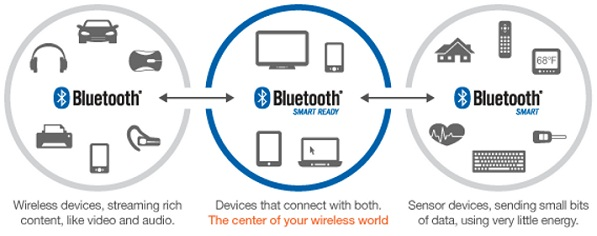
\includegraphics[width=0.9\linewidth, keepaspectratio]{Images/bt/bt_01}
	\caption[Schema di compatibilità.]{Schema di compatibilità tra dispositivi Bluetooth Classic, Smart e Smart Ready.}
	\label{fig:bt_01}
\end{figure}

\begin{figure}[ht]
	\centering
	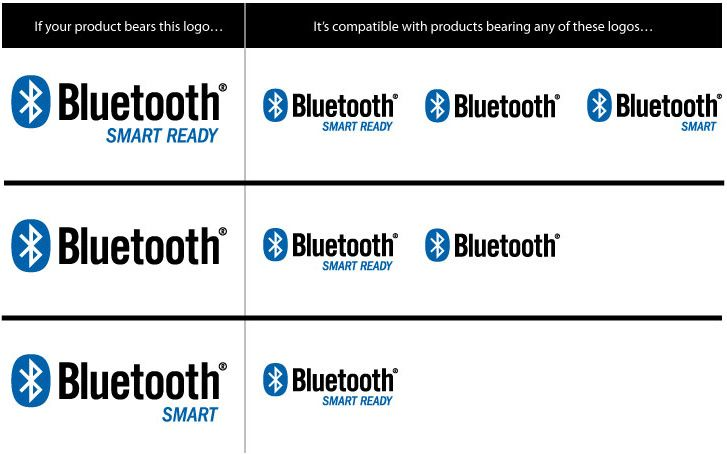
\includegraphics[width=0.9\linewidth, keepaspectratio]{Images/bt/bt_02}
	\caption[Compatibilità tecnologie]{Schema di compatibilità tra tecnologie Bluetooth}
	\label{fig:bt_02}
\end{figure}
Tutti gli smartphone, dal 2010 fino ad oggi sono stati equipaggiati con la tecnologia Low Energy Smart Ready. Si è, infatti, costatato un forte incremento nel mercato, di dispositivi che sfruttano tale tecnologia, come i bracciali con tecnologia fitbit, la serie degli i-Watch e gli smartwatch di Android che rendono l’orologio una vera e propria estensione del telefono. Tutti questi dispositivi sfruttano la tecnologia \acs{BLE} rendendo gestibile l’uso di così tante periferiche Bluetooth senza avere drammatiche conseguenze sulla durata delle batterie. Ora l’azienda Bluetooth SIG sta già lavorando a una nuova versione del \acs{BLE}, la versione 4.1. Essa mira a ridurre alcuni conflitti di banda con la tecnologia \acf{LTE}. Infatti, la 4.0 si trova tra le bande 40 e 41 della tecnologia \acs{LTE}. Per risolvere eventuali conflitti, la nuova versione 4.1 effettua un controllo di banda prima di iniziare le trasmissioni. Uno dei primi smatphone a essere equipaggiato con la nuova versione 4.1 del \acs{BLE} è stato il Google Nexus 6.
\bigskip

 \subsection{Caratteristiche generali}
 
In questa sezione presentiamo, in via generale, alcune caratteristiche del Bluetooth 4.0 Low Energy, anche con qualche comparazione col predecessore Bluetooth Classic per valutare i miglioramenti e i vantaggi che questa nuova tecnologia offre.
%\vskip 3em


%\flushleft\textbf{\textit{Consumo energia}}
\subsubsection{Consumo energia}
La tecnologia \acf{BLE} presenta un consumo ridotto di energia rispetto alla versione precedente, il Bluetooth Classic. Per il Bluetooth Classic vi sono tre classi distinte in cui sono categorizzati i dispositivi, con le relative distanze raggiunte e i consumi associati, mentre per il Bluetooth Low Energy, l’azienda Bluetooth SIG non ha specificato alcun valore massimo di distanza o consumi e quindi il tutto è lasciato come libera scelta ai produttori dei trasmettitori. Questo si traduce ovviamente in una stima per il calcolo del consumo medio di questa nuova tecnologia. Nella \myTab{tab:carBTC} sono riportati i valori di consumi energetici e distanze, relativi al Bluetooth Classic \cite{BT-Basics}, mentre nella \myTab{tab:carBLE} sono riportati i valori di consumo massimo e minimo all'output, per il Bluetooth Low Energy dichiarati nelle specifiche ufficiali \cite{BT-CoreSpec4.0} e il valore stimato medio di distanza raggiungibile presentato in \cite{tesi_tibertoa2013}. Come si può vedere il consumo di energia del Low Energy è ridotto di almeno un ordine di grandezza rispetto al precedente standard Classic.

Come discusso in \cite{sensor2012}, il consumo molto basso da parte del Low Energy, permette a dispositivi alimentati con batterie a bottone, un ciclo di vita che varia tra i 2 giorni e i 14 anni. Inoltre rispetto allo standard Classic, che consente un massimo di 7 dispositivi slave per ogni master, la tecnologia Low Energy offre più flessibilità rendendo questo valore dipendente dall’applicazione e può variare tra 2 e 5.917 slave per master. Riguardo la distanza di trasmissione del \acs{BLE}, è stato stimato essere in media attorno ai 50 metri.
\bigskip
\begin{table}[h]
	\centering
	\begin{tabularx}{\textwidth}{lccc}
		\toprule
		\tableheadline{l}{} &
		\tableheadline{l}{Potenza}(mW) &
		\tableheadline{l}{Potenza}(dBm) &
		\tableheadline{l}{Distanza}(m) \\
		\midrule
		\tablefirstcol{l}{Classe 1}	& 100 & 20 & \textasciitilde100 \\
		\tablefirstcol{l}{Classe 2}	& 2.5 & 4 & \textasciitilde10 \\
		\tablefirstcol{l}{Classe 3}	& 1 & 0 & \textasciitilde1 \\
		\bottomrule
	\end{tabularx}
	\caption[Bluetooth Classic]{Caratteristiche Bluetooth Classic.}
	\label{tab:carBTC}
\end{table}
%\vskip 3em

\begin{table}[ht]
	\centering
	\begin{tabularx}{\textwidth}{ccc}
		\toprule
		\tableheadline{l}{Potenza massima} &
		\tableheadline{l}{Potenza mininima} &
		\tableheadline{l}{Distanza} \\
		\midrule
		10 mW (10 dBm) & 0.01 mW (-20 dBm) & \textasciitilde50 m \\
		\bottomrule
	\end{tabularx}
	\caption[Bluetooth Low Energy]{Caratteristiche Bluetooth Low Energy.}
	\label{tab:carBLE}
\end{table}
%\vskip 5em

\subsubsection{Link Layer}
Come descritto nelle specifiche ufficiali del Bluetooth 4.0\cite{BT-CoreSpec4.0}, l'operatività del Link Layer può essere descritta dai seguenti stati:
\begin{itemize}
	\item Stato di Standby.
	\item Stato di Advertising.
	\item Stato di Scanning.
	\item Stato di Initiating.
	\item Stato di Connection.
\end{itemize}
Questi rappresentano i nodi dell'automa a stati finiti che modella il comportamento del Link Layer. Ogni macchina a stati può essere in un solo stato alla volta, ma un Link Layer può avere più istanze di macchina a stati, se il suo hardware lo consente. È necessario però che almeno una delle sue macchine sia in grado di entrare nello stato di Advertising o nello stato di Scanning. Nel caso di macchine a stati multiple, vi sono restrizioni sulle combinazioni possibili di stati attivi tra tutte le macchine a stati; per ulteriori dettagli si faccia riferimento alla documentazione ufficiale \cite{BT-CoreSpec4.0}.\medskip

Lo stato di Standby è uno stato in cui il dispositivo non trasmette e non riceve alcun pacchetto. Questo stato è raggiungibile da qualsiasi altro stato.\medskip

Lo stato di Advertising, trasmetterà pacchetti di advertising e, se possibile, ascolterà e risponderà a quei pacchetti trasmessi in risposta al suo pacchetto di advertising. Dispositivi nello stato di Advertising sono chiamati advertiser e lo stato di Advertising è raggiungibile dallo stato di Standby.\medskip

Lo stato di Scanning è uno stato di osservazione. Un dispositivo nello stato di Scanning rimane in ascolto per i pacchetti di advertising. Un dispositivo nello stato di Scanning è chiamato scanner e lo stato di Scanning è raggiungibile solo dallo stato di Standby.\medskip

Un Link Layer nello stato di Initiating rimarrà in ascolto per pacchetti di advertising trasmessi da determinati dispositivi e risponderà a determinati pacchetti se ha l’intenzione di aprire una connessione con quel dispositivo mittente. Un dispositivo in stato di Initiating è chiamato initiator. Lo stato di Initiating è raggiungibile dallo stato di Standby.\medskip

Lo stato di Connection può essere raggiunto sia dallo stato di Advertising sia dallo stato di Initiating. Lo stato di Connection si divide a sua volta in due ruoli:
\begin{itemize}
	\item Ruolo Master.
	\item Ruolo Slave.
\end{itemize}
Se raggiunto dallo stato di Advertising si entrerà nello stato di Connection col ruolo di Slave, mentre se si raggiunge lo stato di Connection dallo stato di Initiating si entra nello stato Connection col ruolo di Master.Un singolo dispositivo col ruolo di Slave può comunicare con un solo Master alla volta.
 
In figura \ref{fig:bt_fsa} è riportato lo schema della macchina a stati del Link Layer.
\begin{figure}[t]
	\centering
	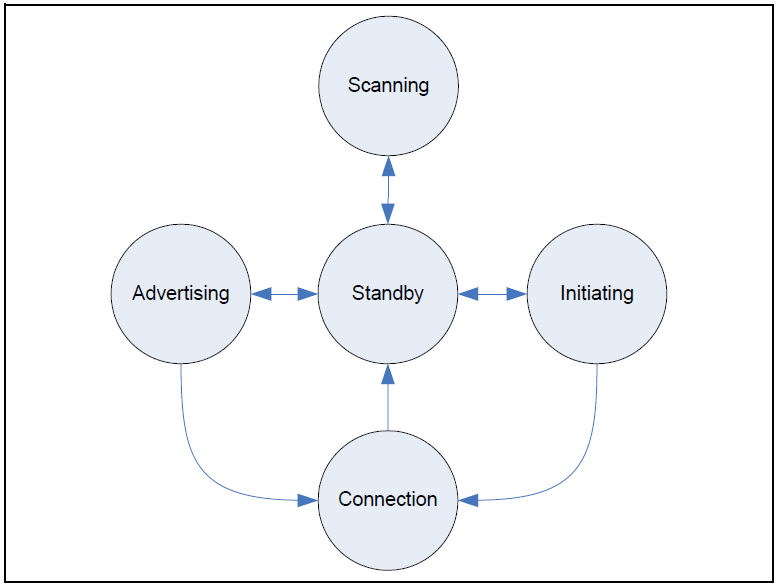
\includegraphics[width=0.9\linewidth, keepaspectratio]{Images/bt/bt_fsa}
	\caption[Schema di compatibilità.]{Schema di compatibilità tra dispositivi Bluetooth Classic, Smart e Smart Ready.}
	\label{fig:bt_fsa}
\end{figure}

\section{Reti Perr-to-Peer}
\subsection{Introduzione}
La nostra ricerca si è orientata su modelli di reti in grado di rappresentare reti \acf{P2P}, chiamate anche Peer2Peer. Una rete P2P è una rete in cui non vi è una struttura gerarchica e ogni nodo è considerato allo stesso livello di tutti gli altri. Senza la presenza di nodi più importanti o nodi rappresentati centri di conoscenza della rete, nessun nodo può avere una visione completa della rete stessa e non può sapere se la porzione di rete da lui vista rappresenta l’intera rete. Ogni nodo quindi, ha una visione parziale e locale dell’overlay della rete. Le topologie di rete sono rappresentate da grafi bidirezionali, poiché i canali di comunicazione tra i nodi di una rete P2P per le situazioni analizzate, sono bidirezionali. Il modello di rete P2P è un’architettura logica di una rete di nodi paritari, senza alcuna struttura Client-Server fissi [\textcolor{red}{\textit{https://it.wikipedia.org/wiki/Peer-to-peer} da cambiare con il riferimento al libro !!}]; ogni nodo è paritario a tutti gli altri, infatti, ogni nodo è chiamato peer. La struttura Client-Server è creata solo nel momento di dover instaurare una connessione tra due nodi, ma più che Client-Server, sarebbe più corretto definirla come Mittente-Destinatario perché non vi sono compiti o azioni predefinite e pre-allocate nelle due parti. Può essere quindi definita una struttura particolare della struttura generica Client-Server.

La principale applicazione di questo modello di rete è stata ed è tuttora quella della condivisione dei file (file sharing), per la quale sono nati tanti sistemi quali Gnutella, FastTrak, Napster, eMule, la rete Torrent, Freenet etc.

Alcune caratteristiche delle reti Peer-to-Peer:
\begin{itemize}
	\item \textit{Basso costo d'implementazione}: non è richiesto l’uso di potenti macchine Server, ma è sufficiente che ogni peer possa sostenere le transazioni dell'utente locale e degli altri peer che vogliono connettersi a lui.
	\item \textit{Amministrazione decentralizzata}: non vi è un server centralizzato di stoccaggio delle informazioni, ma le informazioni sono in possesso dei singoli utenti, localmente, che poi mettono a disposizione della rete.
	\item \textit{Maggiore velocità di trasmissione}: non avendo un Server centralizzato cui tutti i Client si devono connettere per avere un'informazione, causando un calo nella velocità di trasferimento, in un'architettura \acs{P2P} l'informazione può essere reperita anche da più nodi contemporaneamente, infatti, è possibile reperire parti diverse della stessa informazione da nodi diversi e alla fine riassemblare il tutto, col grosso vantaggio di poter avere l'informazione in tempi brevi.
	\item \textit{Sicurezza}: senza la presenza di Server centralizzati, ogni nodo deve garantire per se e per i contenuti che distribuisce, inoltre è anche esposto a ciò che riceve dalla rete che non è controllato da nessuna terza parte. 
\end{itemize}
\vskip 1cm

\subsection{Modelli di Rete}
\label{subsec:modelli_rete}
Poiché abbiamo preso in considerazione l’uso dei grafi, introduciamo due parametri riguardanti i grafi che ne descrivono alcuni aspetti. Essi sono la \textit{edge dependency} e \textit{la degree variance}.
\begin{itemize}
	\item \textbf{\textit{Edge Dependency}}: anche chiamata interdipendenza tra archi. Dato un grafo come in figura \ref{fig:edge_dependency_02}, la edge dependency è definita come la probabilità subordinata che esista un arco tra gli stati S\ped{i}\textasciitilde S\ped{j}, sapendo che esiste un arco tra gli stati S\ped{i}\textasciitilde S\ped{k} e tra S\ped{k}\textasciitilde S\ped{j}. Formalmente, questa probabilità si esprime così P(S\ped{i}\textasciitilde S\ped{j} \textbar\: S\ped{i}\textasciitilde S\ped{k} , S\ped{k}\textasciitilde S\ped{j}) e si può considerare alta se è maggiore della sua probabilità semplice P(S\ped{i}\textasciitilde S\ped{j}).
	\item \textbf{\textit{Degree variance}}: con degree variance s'intende la varianza del grado dei nodi del grafo.
\end{itemize}
\bigskip
\begin{figure}[h]
	\centering
	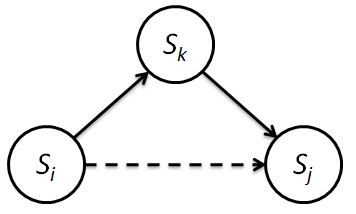
\includegraphics[width=0.8\linewidth,keepaspectratio]{Images/reti/edge_dependency_02}
	\caption[Edge dependency]{Esempio di edge dependency.}
	\label{fig:edge_dependency_02}
\end{figure}
\bigskip
I tre principali modelli di reti presentati in \cite{comparisonGAonRT2012} per la costruzione di reti \acs{P2P} casuali, sono:
\begin{itemize}
	\item Bernoulli Graph.
	\item Random Geometric Graph.
	\item Scale-free Graph.
\end{itemize}
\bigskip

\subsubsection{Bernoulli Graph}
Un Bernoulli Graph \textit{$\beta$(N,p\ped{N})} è un grafo bidirezionale con N nodi nel quale le connessioni hanno una probabilità di esistere pari a p\ped{N}. Per ogni coppia di nodi vi è una probabilità pN che il link tra loro esista, indipendentemente da ogni altra connessione. In figura \ref{fig:bernoulli_graph} è riportato un esempio. Un Bernoulli Graph presenta bassa edge dependency e bassa degree variance.
\bigskip
\begin{figure}[h]
	\centering
	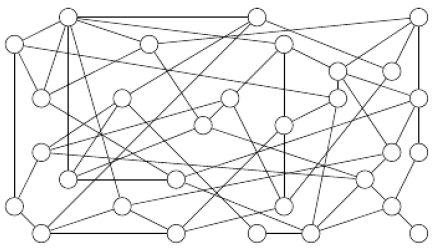
\includegraphics[width=0.7\linewidth,keepaspectratio]{Images/reti/bernoulli_graph}
	\caption[Bernoulli graph]{Esempio di Bernoulli graph.}
	\label{fig:bernoulli_graph}
\end{figure}
\bigskip

\subsubsection{Random Geometric Graph}
\label{subsubsec:rgg}
Un \acf{RGG} \textit{G(N,$ \rho $)} è un grafo bidirezionale casuale inserito in un'area limitata. Il grafo è generato disponendo in maniera casuale e uniforme gli N nodi all'interno dell'area. Poi due nodi sono connessi se essi tra loro se essi si trovano a una distanza geometrica pari o inferiore a \textit{$ \rho $}. In figura \ref{fig:RandomGeometricGraph} è riportato un esempio. E' facile notare come reti di questo tipo siano estremamente adatte alla rappresentazione di reti wireless, caratterizzate dalla distanza fisica tra i nodi e da un valore soglia \textit{$ \rho $} entro il quale è possibile eseguire trasmissioni. Un \acs{RGG} presenta un'alta edge dependency, dovuta all'importanza della vicinanza fisica tra i nodi, e una bassa degree variance.
\begin{figure}[h]
	\centering
	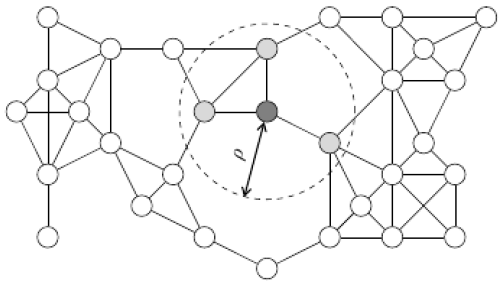
\includegraphics[width=0.7\linewidth,keepaspectratio]{Images/reti/RandomGeometricGraph}
	\caption[Random Geometric grah]{Esempio di Random Geometric graph.}
	\label{fig:RandomGeometricGraph}
\end{figure}
\bigskip

\subsubsection{Scale-free Graph}
Un Scale-free Graph \textit{S(N,m)} è un grafo bidirezionale con una bassa edge dependency e un'alta degree variance, dovuta alle sue connessioni distribuite secondo legge potenza. Reti di questo tipo sono generate partendo con un set di nodi m\ped{0}, poi a ogni ciclo si aggiunge un nodo e si collegano i suoi m archi ad altri nodi già presenti nel grafo. La probabilità che un nuovo nodo sia collegato a un nodo già esistente è proporzionale al grado di quest'ultimo. Collegamenti di questo tipo si dicono preferenziali e fanno si che si creino pochi nodi, chiamati \textit{hub}, con un grado medio alto di circa 2 \textit{m}, e molti nodi chiamati \textit{periferici}, con grado medio compreso tra \textit{m} e 2 \textit{m}. In figura \ref{fig:scale-free} è riportato un esempio.
\bigskip
\begin{figure}[h]
	\centering
	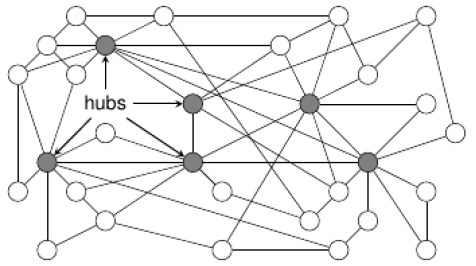
\includegraphics[width=0.7\linewidth,keepaspectratio]{Images/reti/scale-free}
	\caption[Scale-free graph]{Esempio di Scale-free graph.}
	\label{fig:scale-free}
\end{figure}


\section{Algoritmi di Gossip}
I protocolli Epidemici, o di Gossip, sono paradigmi computazionali e di comunicazione orientati a sistemi distribuiti su larga scala caratterizzati da alta dinamicità. Il metodo più semplice per la diffusione d’informazioni in una rete è effettuare un broadcast cercando di propagare al maggior numero di nodi l’informazione, ma con lo svantaggio di saturare tutti i canali di comunicazione. Per questo motivo i protocolli di gossip utilizzano un approccio probabilistico per la gestione della diffusione dell’informazione attraverso la rete, con lo scopo di massimizzare la diffusione dell’informazione sovraccaricando il meno possibile i canali di comunicazione. In un protocollo epidemico, un nodo che ha un’informazione sceglierà in modo casuale un nodo vicino con cui comunicare e tentare di condividere l’informazione.

Uno dei protocolli epidemici più famoso è “Game of life” \cite{gardner1970-gameoflife}, un automa cellulare sviluppato dal matematico inglese John Conway sul finire degli anni sessanta. L'ambiente per quest'algoritmo è un insieme di celle, dove ogni cella ha 8 celle vicine come mostrato in figura 2.5. Lo scopo dell'algoritmo è di diffondere il seme della vita, quindi ogni cella può essere occupata o no in base alle seguenti regole:
\begin{itemize}
	\item Nascita: se una cella non occupata ha tre celle vicine occupate, diventa anch’essa occupata.
	\item Morte: se una cella occupata ha 0 o 1 cella vicina occupata, muore di solitudine, oppure se ha dalle 4 alle 8 celle vicine occupate, muore di sovraffollamento.
	\item Sopravvissuta: se una cella occupata ha 2 o 3 celle vicine occupate, essa sopravvive alla generazione successiva.
\end{itemize}

\begin{figure}[bh]
\centering
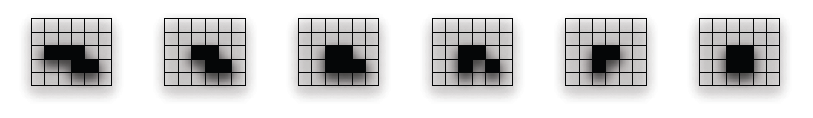
\includegraphics[width=1\linewidth,keepaspectratio]{Images/algoritmi_gossip/game_of_life}
\caption[Game of Life]{Algoritmo Game of Life}
\label{fig:game_of_life}
\end{figure}

\subsection{Classificazione degli algoritmi epidemici}
Come discusso in \cite{schindel2004-epidemicAlg} in ogni algoritmo epidemico vi è quella che è chiamata popolazione, un insieme di unità interattive comunicanti. Queste unità usano un set di regole che specificano le modalità di diffusione di una specifica informazione ad altre unità. La scelta di queste regole è molto legata al tipo di algoritmo e al comportamento che quest'ultimo deve avere. L'importante è che a ogni istante di tempo t, ogni unità sia in uno dei seguenti tre stati, riguardo a una specifica informazione:
\begin{itemize}
		\item Suscettible (suscettibile): l’unità non conosce nulla dell’informazione in questione ma è disposta a venirne a conoscenza.
		\item Infected (contagiata): l’unità è a completa conoscenza dell’informazione in questione e utilizza il set di regole per diffondere a sua volta l’informazione.
		\item Removed (Rimossa): l’unità è a completa conoscenza dell’informazione in questione ma non la diffonde.
\end{itemize}
Sulla base delle definizioni appena descritte, possiamo definire diverse classi di algoritmi, in cui è indicato per ogni classe come in generale sono trattate le informazioni.

Le principali classi sono:
\begin{itemize}
	\item \acf{SI}.
	\item \acf{SIS}.
	\item \acf{SIR}.
	
\end{itemize}
Esistono anche altre classi che estendono ulteriormente queste classi, aggiungendo alcuni stati intermedi.

In modelli \textbf{\textit{\acf{SI}}} si ha che i nodi possono essere suscettibili a un’informazione e quando ne vengono a conoscenza, diventano contagiati e vi rimangono fintanto che tutta la popolazione non diventa contagiata. Ciò però richiede ulteriori controlli esterni per decidere quando terminare la diffusione dell’informazione.

A differenza del modello \acs{SI}, in quello \textbf{\textit{\acf{SIS}}} un’unità contagiata può decidere di fermare la diffusione dell’informazione prima che tutta la popolazione sia contagiata. Ogni unità rimossa può tornare a essere contagiata se riceve nuovamente l’informazione che aveva smesso di trasmettere e ricominciare a trasmetterla di nuovo finché non perde nuovamente interesse nel farlo.

Il modello \textbf{\textit{\acf{SIR}}} è molto simile al modello \acs{SIS}, con la differenza che un’unità rimossa rimane rimossa per sempre per quella determinata informazione e non potrà più esser contagiata da quell’informazione. Ciò non impedisce che tale unità possa diventare poi suscettibile a nuove informazioni.

\subsection{Medoti di diffusione}
In generale, ogni algoritmo di gossip prevede che a ogni iterazione dell’algoritmo ogni unità della popolazione se deve comunicare con un nodo, esso sia scelto in maniera casuale tra i nodi dell’intera popolazione. Poi ogni algoritmo specifica, con vincoli più stringenti, regole diverse di selezione del destinatario. In generale però vi sono tre metodi con cui le unità di una popolazione possono diffondere le informazioni ad altre unità:
\begin{itemize}
	\item Push.
	\item Pull.
	\item Push\&Pull.
\end{itemize}
\bigskip

\noindent\textbf{Metodo Push}\\
L'algoritmo Push prevede che i nodi contagiati prendano l’iniziativa di diffondere l’informazione, quindi a ogni istante t, il nodo contagiato sceglie un nodo casuale e prova a contagiarlo, come mostrato in figura \ref{fig:push}. Questa strategia è molto efficace all’inizio della diffusione, quando vi è un alto numero di unità suscettibili e poche contagiate o rimosse, quindi la probabilità che ogni nodo contagiato ha di scegliere un nodo suscettibile è alta. Questa probabilità decresce col passare del tempo perché la quantità di nodi suscettibili diminuisce e il numero di nodi contagiati o rimossi aumenta, rendendo questo metodo poco affidabile nel lungo periodo. Questo metodo non garantisce che tutta la popolazione sia contagiata.
\bigskip
\begin{figure}[bh]
\centering
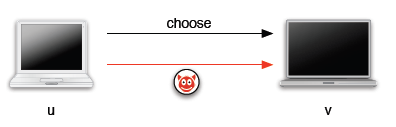
\includegraphics[width=0.7\linewidth,keepaspectratio]{Images/algoritmi_gossip/push}
\caption[Metodo di Push]{Metodo di Push.}
\label{fig:push}
\end{figure}
\bigskip


\noindent\textbf{Metodo Pull}\\
L'algoritmo Pull prevede che un nodo contagiato non si muova attivamente nel diffondere l'informazione, ma che siano i nodi suscettibili a fare richiesta di nuove informazioni ai nodi contagiati. A ogni istante t, un nodo suscettibile seleziona casualmente un altro nodo e gli chiede se ha nuove informazioni. Se il nodo contattato ne ha, allora restituisce l'informazione; in figura \ref{fig:pull} è riportato un esempio. Quest'algoritmo di propagazione è poco efficace all'inizio dell'epidemia perché vi è solo un nodo contagiato e la probabilità di scegliere proprio lui è uno sulla grandezza della popolazione. Col passare del tempo, più l'informazione si diffonde, più alta sarà la probabilità di selezionare un nodo contagiato. Questo metodo non garantisce che il processo di diffusione abbia inizio poiché vi è una probabilità che nessun nodo suscettibile contatti il nodo contagiato, ma vi è anche la possibilità che tutti i nodi scelgano il nodo contagiato generando così un rapido inizio di epidemia. Questo metodo però garantisce che, se l'epidemia inizia, essa si diffonderà a tutta la popolazione.
\bigskip
\begin{figure}[h]
	\centering
	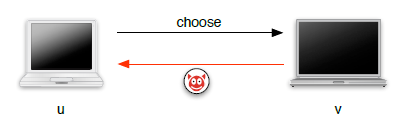
\includegraphics[width=0.7\linewidth,keepaspectratio]{Images/algoritmi_gossip/pull}
	\caption[Metodo di Pull]{Metodo di Pull.}
	\label{fig:pull}
\end{figure}
\bigskip


\noindent\textbf{Metodo Push\&Pull}\\
I metodi Push e Pull presentano vantaggi e svantaggi in differenti momenti del processo di diffusione, l'unione dei due ha lo scopo di combinare i vantaggi dei due metodi. In questo caso un nodo contagiato utilizzerà una strategia Push, mentre i nodi suscettibili utilizzeranno una approccio Pull finché non saranno contagiati. Nelle prime fasi della diffusione premierà più la strategià Pulsh, mentre a contagio avanzato si sentirà di più la strategia di Pull. In figura \ref{fig:push_pull} è rappresentato un esempio di strategia Push\&Pull.
\bigskip
\begin{figure}[h]
	\centering
	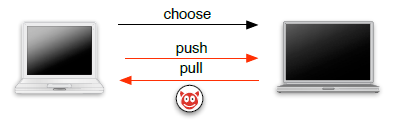
\includegraphics[width=0.7\linewidth,keepaspectratio]{Images/algoritmi_gossip/push_pull}
	\caption[Metodo di Push\&Pull]{Metodo di Push\&Pull.}
	\label{fig:push_pull}
\end{figure}
\bigskip

\subsection{Applicazioni}
Il letteratura vi sono molti esempi di applicazioni degli algoritmi di gossip, tra i tanti citiamo quello per il corretto Replicated Database Maintenance \cite{montresor2004-antiEntropy}, l’Epidemic Routing e il Mantenimento della visione del Network Overlay \cite{montresor2004-overlay}. In merito al Replicated Database Maintenance il primo algoritmo studiato fu il Direct Mail, una soluzione che prevede che il nodo in possesso della nuova informazione debba contattare direttamente ogni altro nodo per diffondere l’aggiornamento. Questo metodo è posso affidabile perché è molto sensibile allo stato della rete su un unico nodo e sull’unico mittente. Per ovviare a tali problemi sono stati introdotti due principali algoritmi di gossip: Anti-Entropy e il Rumor Mongering. L’Anti-Entropy è un algoritmo di tipo SI, che cerca come dice il nome di contrastare la crescita dell’entropia in un sistema di replicazione dati, facendo si che a ogni ciclo dell’algoritmo, a coppie, i nodi sincronizzino i loro dati. Unico problema è che per la sincronizzazione di database, a volte è necessario trasmettere sulla rete l’intero database. Il Rumor Mongering invece è un algoritmo di tipo SIR che ha lo scopo di propagare tra i nodi solo l’elenco degli aggiornamenti e mai l’intero database. A ogni ciclo ogni nodo che ha la lista aggiornamento non vuota, sceglie un nodo casuale e cerca di propagargli i suoi aggiornamenti. Con questo tipo di algoritmo nasce il problema di trovare un criterio col quale decidere quando smettere di propagare gli aggiornamenti.
 
Da questo sono nati diverse versioni dell’algoritmo di Rumor Mongering, in base ai diversi criteri usati per fermare la propagazione degli aggiornamenti. E’ quindi possibile suddividere la classe degli algoritmi di Rumor Mongering nelle seguenti sotto classi:
\begin{itemize}
	\item \textbf{\textit{Blind}}: un nodo contagiato decide di interrompere la diffusione in base al suo stato interno.
	\item \textbf{\textit{Feedbackind}}: un nodo contattato risponde dicendo se già conosce oppure no l’informazione. Il nodo contagiato mittente, in base alla risposta prende una decisione.
	\item \textbf{\textit{Coin}}: il nodo contagiato si fermerà con una probabilità 1/k, dove k è il numero di nodi contattati.
	\item \textbf{\textit{Counter}}: il nodo contagiato incrementa un contatore per ogni informazione inviata con successo. Si ferma quando il contatore supera una soglia prefissata.
\end{itemize}

\subsection{Algoritmi di gossip per il Peer2Peer}
\label{subsec:alg_p2p}
Nel contesto degli algoritmi di gossip relativi a reti \acs{P2P}, presenteremo quelli più utilizzati per la diffusione di messaggi e discussi in \cite{comparisonGAonRT2012} e \cite{comparisonGAonRT2014-ita}. Essi sono il \acf{PB}, \acf{PE} e \acf{FF}. Definiti i seguenti termini:
\begin{itemize}
	\item $ \varLambda_{i} $: insieme di nodi adiacente all’i-esimo nodo.
	\item \textit{V\ped{i}}: la cardinalità di $ \Lambda_{i} $.
	\item \textit{msg}: il messaggio da diffondere.
	\item \textit{p\ped{v},p\ped{e},fanout}: sono i valori probabilistici a ciascun algoritmo, rispettivamente PB,PE e FF.
\end{itemize}
\bigskip

\noindent\textbf{\acf{PB}}\\
Il Probabilistic Broadcast, prevedere che chi ha l'informazione o la ricevuta, la diffonda con una certa probabilità pv ai nodi vicini. L'algoritmo \ref{alg:gossipPB} descrive in pseudo codice il funzionamento di questo metodo.
\bigskip
\begin{algorithm}[h]
	\caption{Probabilistic Broadcast}\label{alg:gossipPB}
	\begin{algorithmic}[1]
		\Function{GossipPB}{msg,\emph{p\ped{v}}}
			\If{Random() $ \leq $ \textit{p\ped{v}}}
				\ForAll{$ \textit{s}_\textit{i} \in \Lambda_{i} $}
					\State Send(msg,\emph{s\ped{j}})
				\EndFor
			\EndIf
		\EndFunction
	\end{algorithmic}
\end{algorithm}
\bigskip

\noindent\textbf{\acf{PE}}\\
Il Probabilistic Edge, prevedere che chi ha l'informazione o l'ha ricevuta, la diffonda su ogni arco uscente con una certa probabilità pe per ogni arco. L'algoritmo \ref{alg:gossipPE} è lo pseudo codice che descrive il funzionamento.
\bigskip
\begin{algorithm}[h]
	\caption{Probabilistic Edge}\label{alg:gossipPE}
	\begin{algorithmic}[1]
		\Function{GossipPE}{msg,\emph{p\ped{e}}}
			\ForAll{$ \textit{s}_\textit{j} \in \Lambda_{i} $}
				\If{Random() $ \leq $ \textit{p\ped{e}}}
					\State Send(msg,\emph{s\ped{j}})
				\EndIf
			\EndFor
		\EndFunction
	\end{algorithmic}
\end{algorithm}
\bigskip

\noindent\textbf{\acf{FF}}\\
Il Fixed Fanout, prevedere che chi ha l’informazione o l’ha ricevuta, la diffonda a fanout nodi adiacenti selezionati a caso tra tutti i nodi vicini. L'algoritmo \ref{alg:gossipFF} descrive tramite pseudo codice il funzionamento di questo metodo.
\bigskip
\begin{algorithm}[h]
	\caption{Fixed Fanout}\label{alg:gossipFF}
	\begin{algorithmic}[1]
		\Function{GossipPE}{msg,\emph{fanout}}
			\If{$ \textit{fanout} \geq \textit{V}_\textit{i} $}
				\State $ \textit{toSend} \gets \Lambda_i $
			\Else
				\State $ \textit{toSend} \gets \emptyset $
				\For{$ \textit{f} = 1 \;\textbf{to}\; \textit{fanout}$}
					\State random select $ \textit{s}_\textit{j} \in \Lambda_{i}/\textit{toSend} $
					\State $ \textit{toSend} \gets \textit{toSend}\bigcup \textit{s}_\textit{j}$
				\EndFor
			\EndIf
			\ForAll{$ \textit{s}_\textit{j} \in \textit{toSend}$}
				\State Send(msg,\emph{s\ped{j}})
			\EndFor
		\EndFunction
	\end{algorithmic}
\end{algorithm}
\bigskip


\section{Simulatori}
\label{sec:simulatori}
La nostra ricerca si è focalizzata su simulatori di reti Peer-2-Peer, reti in cui tutti i nodi della rete sono allo stesso livello, sono paritetici e non vi è presenza di gerarchie tra nodi, e su simulatori di protocolli basati sia su cicli sia su eventi. In generale simulare qualcosa prevede l'esecuzione di una sequenza di operazioni nel tempo e, dove le entità che eseguono tali operazioni sono molteplici. Per poter gestire l'esecuzione contemporanea e/o concorrente di più entità il simulatore deve stabilire l'ordine in cui eseguire quale istruzione di quale nodo. La scelta sul come venga stabilito l’ordine di esecuzione caratterizza il motore del simulatore che potrà essere basato su cicli, su eventi o su entrambi. Una simulazione basata su cicli prevede che si definisca uno “time step” di simulazione, che è l'incremento del tempo virtuale di simulazione che definisce la cadenza di ogni ciclo. Tutte le operazioni definite come periodiche verranno eseguite ad ogni ciclo, contemporaneamente. Inoltre qualsiasi evento non periodico che occorre tra un ciclo e un altro verrà schedulato al ciclo successivo. Come si vede in figura \ref{fig:cycled_driven_01}, gli eventi e\ped{0}, e\ped{1} ed e\ped{2} accadono tra un ciclo e il successivo, con un passo di simulazione di $\Delta t$. L'evento e0 verrà quindi processato all'instante $\Delta t$, mentre gli eventi e\ped{1} ed e\ped{2} verranno processati all'instante $4\Delta t$. In questo modo si perde la distribuzione degli eventi, avendo lo scheduler che appiattisce la distribuzione temporale su un unico ciclo, ad ogni iterazione. Questo tipo di simulazioni sono molto vincolanti e non permettono una rappresentazione realistica di una generica classe di nodi. Si adatta molto bene a simulazioni di operazioni batch e/o periodiche. Per poter avere più precisione e dettaglio nella modellazione dell'esecuzione degli eventi vi è lo scheduling guidato dagli eventi che, come dice il nome, ordinerà le operazioni da eseguire in base al momento in cui esse hanno generato o genereranno un evento.

In figura \ref{fig:event_driven_01} è riportato un esempio di scheduling guidato dagli eventi. Il tempo di simulazione non sarà più una progressione costante, ma seguirà il susseguirsi degli eventi, nell'ordine in cui essi avvengono. In questo caso la simulazione avrà inizio con l'evento e\ped{0}, poi il simulatore salterà all'instante di tempo t1 in quanto lo scheduler prima di t\ped{1} non ha nessuna operazione che deve essere eseguita.

\begin{figure}[t]
	\centering
	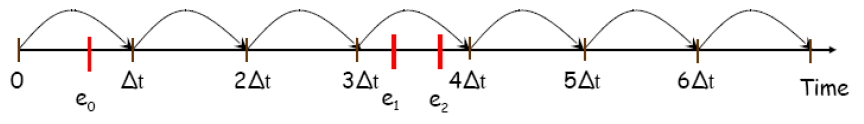
\includegraphics[width=0.9\linewidth, keepaspectratio]{Images/simulatori/cycled_driven_01}
	\caption[Cycle driven scheduling]{Scheduling guidato dai cicli.}
	\label{fig:cycled_driven_01}
\end{figure}

\begin{figure}[t]
	\centering
	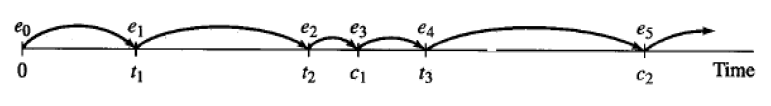
\includegraphics[width=0.9\linewidth, keepaspectratio]{Images/simulatori/event_driven_01}
	\caption[Event driven scheduling]{Scheduling guidato dagli eventi.}
	\label{fig:event_driven_01}
\end{figure}

All'istante t\ped{1} avviene l'evento e\ped{1} e viene processato, poi si passerà all'istante di tempo t\ped{2} perché l'evento e\ped{2} è previsto che avvenga in quell'istante e così via tutti gli altri. In generale gli eventi sono relativi per esempio alla ricezione di un messaggio da parte di un nodo. In figura \ref{fig:event_driven_01} vediamo che vi sono gli eventi e\ped{3} ed e\ped{5} che sono schedulati agli istanti di tempo c\ped{1} e c\ped{2}. Questo è un esempio di integrazione di eventi ciclici in un ambiente guidato dagli eventi. Gli eventi e\ped{3} ed e\ped{5} sono azioni periodiche e quindi devono essere eseguite ogni “time step” specificato, ma come fare se non vi è un “time step” di simulazione? Il simulatore genererà un evento ogni “time step” di tempo di simulazione associando come evento l'azione periodica. Ciò garantisce di poter avere con un unico motore di scheduling, sia eventi aperiodici che azioni periodiche. In questo caso abbiamo un simulatore basato sia sugli eventi sia sui cicli.

In letteratura esistono tanti simulatori di reti come Mosquite\footnote{\url{http://www.mesquite.com/}} che è una libreria per CSIM, PADS\footnote{\url{http://pads.cs.unibo.it/doku.php?id=start/}} sviluppato dal Dipartimento di Ingegneria Informatica dell’Università di Bologna in grado di simulare protocolli complessi su reti di larga scala o senza una ben definita struttura. Vi è anche PeerSim\footnote{\url{http://peersim.sourceforge.net/}} una libreria Java che fornisce gli strumenti di simulazione basata sia su cicli sia su eventi. Abbiamo poi concentato la nostra attenzione su OMNeT++\footnote{\url{http://omnetpp.org/}}, un framework costruito sulla piattaforma Eclipse\footnote{\url{https://eclipse.org/}} ma scritto in C++. OMNeT++ è uno simulatore basato solo su eventi ma dato il suo intenso sviluppo in ambito commerciale, vi sono disponibili diverse librerie e tool in grado di offrire molte funzionalità di simulazione di protocolli di rete e diverse tipologie di reti. Nel seguito presenteremo brevemente le caratteristiche di PeerSime e OMNeT++.

\subsection{PeerSim}
PeerSim è un software sviluppato in ambiente accademico che consente di simulare reti con una alta flessibilità sul numero di nodi che compongono la rete, rendendolo quindi adatto a simulare reti di grandi dimensioni. In letteratura troviamo diversi riferimenti e trattazioni in merito a questo software, come \cite{montresor2010-peersim}, \cite{montresor2009-peersim_scalabile} e \cite{montresor2009-peersimP2P}. PeerSim poi necessita che venga definito lo stack di protocolli che ogni nodo della rete implementerà; infatti la logica con cui questo simulatore costruisce la rete da simulare è quella di istanziare solo un nodo e poi esso viene copiato, o clonato, tante volte fino a raggiungere il numero di nodi nella rete. Per questo motivo si nota subito  che PeerSim è uno strumento ottimizzato per la simulazione di reti anche di grandi dimensioni e soprattutto, come si può dedurre dal nome, reti soprattutto Peer-to-Peer \cite{montresor2009-peersimP2P}. Non presenta alcun tipo di strumento grafico per la rappresentazione della rete o dei pacchetti in transito tra i nodi, la simulazione è solo computazione e stampa messaggi su console. Vi è la possibilità di utilizzare o estendere alcune funzioni di alcuni componenti del sistema di simulazione che permettono di stampare su file di testo le coordinate dei nodi della rete e/o i rami del grafo della rete nel formato usato da GNUplot\footnote{\url{http://www.gnuplot.info/}} e quindi poi visualizzare il layout di rete. PeerSim necessita che l’utente definisca in un apposito file di configurazione le specifiche di simulazione, della rete, dei protocolli implementati sui nodi, delle dipendenze tra i protocolli. Richiede inoltre di specificare i componenti di inizializzazione, i componenti di controllo e i componenti di osservazione. I componenti di inizializzazione sono componenti che il simulatore eseguirà solo all’inizio del processo di simulazione e hanno il compito di inizializzare i nodi della rete e la rete stessa, ad esempio per stabilire le connessioni tra i nodi. I componenti di controllo sono “agenti” che vengono eseguiti ciclicamente e hanno il compito di agire sulla rete durante la simulazione, per introdurre dinamicità nella stessa come per esempio accendere o spegnere nodi o canali di trasmissione per simulare malfunzionamenti oppure aggiungere o togliere nodi e collegamenti. Questi componenti di controllo sono opzionali. Infine i componenti di osservazione detti anche osservatori sono componenti che operano alla fine della simulazione oppure ciclicamente se resi cycle-based impostando il loro time step. Il loro compito è quello appunto di osservare la rete e permettere di raccogliere dati per analisi. I dati da raccogliere devono essere specificati dall’utente nell’apposita funzione di osservazione che viene eseguita dal motore di simulazione. Un esempio di osservatore è il componente che permette di scrivere su file il layout della rete in formato compatibile con GNUplot. Punto forte di questo simulatore quindi sono la flessibilità sul numero di nodi della rete, le ottime prestazioni di simulazione anche per grandi reti e la scelta di lasciare all’utente l’estensione dei componenti che governano la simulazione.
\bigskip

\subsection{OMNeT++}
OMNeT++ è un framework e libreria di simulazione basata sul linguaggio C++, estendibile e modulare. OMNeT++ è un software di simulazione molto diffuso sia nel settore commerciale sia nel settore scientifico per la simulazione di reti e protocolli di trasmissione, disponibile dal 1997. OMNeT++ è un software che offre un editor di sviluppo basato su Eclipse. Sono disponibili una gran varietà di strutture base come reti wired e wireless ed è possibile aggiungere estensioni che permettono di ampliare la gamma di reti supportate. INET è una delle estensioni più corpose del framework e contiene una grossa quantità di reti e protocolli delle più diffuse strutture di rete utilizzate. Vi sono molte trattazioni in letteratura riguardo a questo strumento, come \cite{omnet2010-book}, \cite{omnet2002-overview} fino a uno studio per uso didattico \cite{omnet2002-edu}.

OMNeT++ è un simulatore di eventi discreti, ma come spiegato all'inizio di questa sezione, è possibile coprire anche situazioni di esecuzione di azioni periodiche, organizzandole come eventi programmati. OMNeT++ contiene anche un ambiente grafico \cite{omnet2002-overview}, Tkenv, per la rappresentazione grafica della struttura della rete e degli eventuali link fisici tra i nodi; è in grado inoltre di eseguire un ri-ordinamento spaziale dei nodi della rete con l’obiettivo di rappresentare il grafico della rete col minor numero di intersezioni tra i collegamenti possibili, per rendere più leggibili lo schema ed eventuali animazioni date dalla simulazione. In \myFig{fig:tkenv_01} è riportato un esempio.
\begin{figure}[tb]
\centering
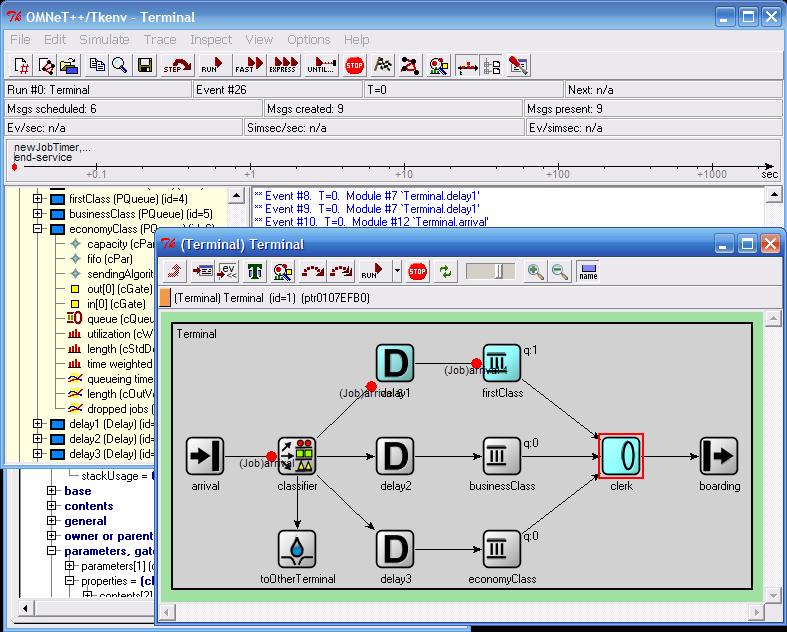
\includegraphics[width=0.7\linewidth]{Images/omnet/tkenv_01}
\caption[tkenv]{Esempio di rappresentazione tramite Tkenv.}
\label{fig:tkenv_01}
\end{figure}
OMNeT++ offre una architettura modulare, cercando di perseguire il principio di riutilizzo dei moduli\cite{omnet2002-overview}. Ogni modulo corrisponde ad un singolo componente della rete o a un componente aggregato, composto a suoa volta da componenti singoli. In questo modo è possibile costruire reti su più livelli, e poter analizzare la rete da punti di vista di diverse granularità. Il linguaggio di alto livello utilizzato per descrivere i moduli si chiama \acf{NED}. La struttura è definita in linguaggio \acs{NED}, mentre il comportamento dei moduli e dei componenti è scritto utilizzando sempre il C++, nei rispettivi file. 
Con OMNeT++, come per PeerSim,  è possibile specificare in appositi file di inizializzazione una lista di parametri necessari a configurare la rete durante la sua fase di inizializzazione prima di iniziare la simulazione vera e propria.  In un singolo file di inizializzazione è possibile specificare più scenari di esecuzione e per ognuno specificare quindi valori diversi. I parametri specificati possono essere letti dal file di Network Definition e usati per creare e impostare la rete secondo i parametri specificati dall’utente nel file di inizializzazione. Tramite il file di Network Definition si può propagare la lettura dei parametri fino ai file C++ con le procedure che modellano il comportamento del componente.
OMNeT++ offre anche un sistema di raccolta dati, tramite il quale si possono poi analizzare i dati raccolti, filtrarli e ottenere differenti rappresentazioni grafiche dei dati stessi \cite{omnet2002-overview}. La raccolta dati può essere sia la sequenza temporale dei risultati, sia una raccolta delle statistiche su dati specifici oppure entrambe le cose.
 \bigskip
 
\subsubsection{File di Inizializzazione}
Un file di inizializzazione è un file necessario alla corretta configurazione della rete, dei suoi componenti e dell'ambiente di simulazione. Un file di inizializzazione ha estensione “.ini” e per comodità verrà anche chiamato “INI file”. In un file di inizializzazione è possibile fornire parametri organizzati in una struttura ad albero, in cui ogni ramo  è uno scenario di simulazione indipendente dagli altri ma eredita tutti i parametri coi rispettivi valori, se non vengono ridefiniti, dello scenario padre. Al momento della simulazione vera e propria, il sistema chiederà all'utente di scegliere quale scenario di simulazione utilizzare se non ve ne è uno specificato direttamente nello script che lancia l'esecuzione di simulazione. 
Nella figura \ref{fig:ini_file} sono riportati due esempi di file d'inizializzazione. Vediamo nella figura \ref{subfig-1:tictoc_ini_01} come sotto la sezione “General” vengano specificati tutti i parametri comuni a tutte le configurazioni e di seguito vengono specificate tutte le altre configurazioni coi parametri specifici per quelle simulazioni. Mentre nella figura \ref{subfig-2:tictoc_ini_02} è riportata una possibile struttura ad albero delle configurazioni.

\begin{figure}[t]
	\subfloat[\label{subfig-1:tictoc_ini_01}]{%
		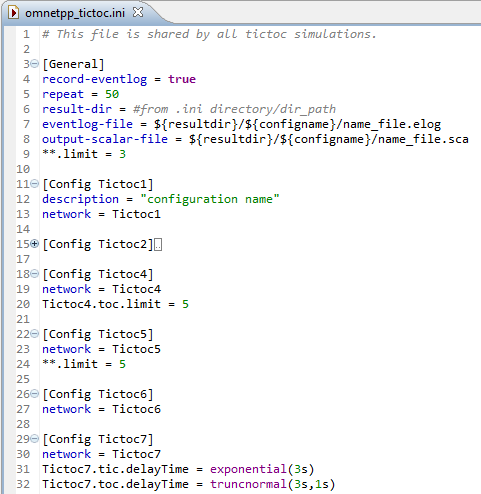
\includegraphics[width=0.45\textwidth, keepaspectratio]{Images/omnet/tictoc_ini_01}
	}
	\hfill
	\subfloat[\label{subfig-2:tictoc_ini_02}]{%
		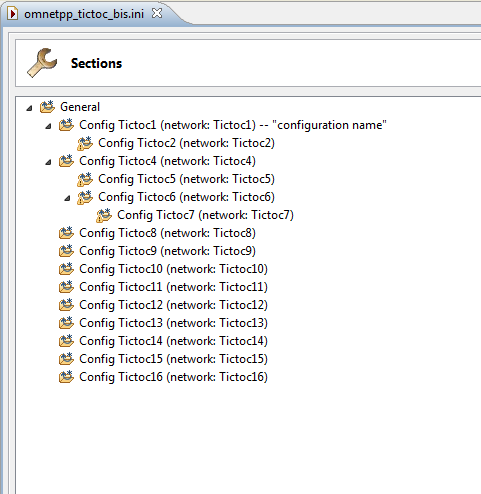
\includegraphics[width=0.45\textwidth, keepaspectratio]{Images/omnet/tictoc_ini_02}
	}
	\caption{Esempio di file di inizializzazione.}
	\label{fig:ini_file}
\end{figure}

In generale ogni file di inizializzazione caratterizza un set di scenari da simulare, quindi si tende a includere nella sezione “General” anche tutti i parametri che servono a impostare correttamente la simulazione o la gestione del framework quali, per esempio l'unità di misura con la quale viene scandito il tempo di simulazione, il numero di ripetizioni per ogni caso di studio che si desidera fare, le varie directory in cui si vogliono salvare i risultati o i dati raccolti.

\subsubsection{Linguaggio NED}
OMNeT++ offre, tramite un linguaggio ad alto livello chiamato Network Definition, la possibilità di definire il layout della rete e la struttura dei singoli componenti e della composizione dei componenti più grandi. Il linguaggio di Network Definition viene usato per creare file di specifica con estensione “.ned”, che abbrevieremo con NED file. Il linguaggio NED è stato pensato per poter implementare singoli moduli in maniera indipendente dall’ambiente, rendendo così facile il loro riutilizzo o estensione. Il sistema ci offre due visibilità del layout di rete ad alto livello: Design e Source. Con la vista Design viene fornita una rappresentazione grafica della rete, se pur sempre ad alto livello, mentre la vista Source permette di vedere e implementare il file come puro codice sorgente. In \myFig{subfig-1:tictoc_ned_01} è riportato un esempio di NED file in vista Design, dove il sistema dice che nel file in questione sono stati usati componenti di tipo “Txc11”, i canali di comunicazioni utilizzati sono dei “Channel” e la rete si può riassumere come un vettore di nodi collegati tra di essi tramite diversi “Channel”. La vera rappresentazione del layout di rete viene fatta solo a runtime in fase di simulazione nel caso venga utilizzato lo strumento grafico Tkenv. In figura \myFig{subfig-2:tictoc_ned_02} invece è riportato lo stesso file della \myFig{subfig-1:tictoc_ned_01} ma in vista Source. Come si può vedere nella figura \myFig{subfig-2:tictoc_ned_02}, in vista sorgente possiamo vedere tutto il codice corrispondente alla vista Design. Si nota che nella prima parte viene definito il singolo componente “Txc11”, poi viene definita la rete come un vettore di componenti “Txc11” e tra essi vi sono dei collegamenti di tipo “Channel”, che è definito dentro la rete.
\bigskip
\begin{figure}[t]
	\subfloat[Vista Design.\label{subfig-1:tictoc_ned_01}]{%
		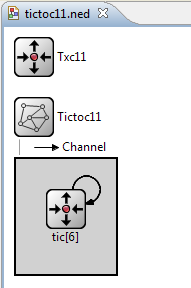
\includegraphics[width=0.38\textwidth, keepaspectratio]{Images/omnet/tictoc_ned_01}
	}
	\hfill
	\subfloat[Vista Source.\label{subfig-2:tictoc_ned_02}]{%
		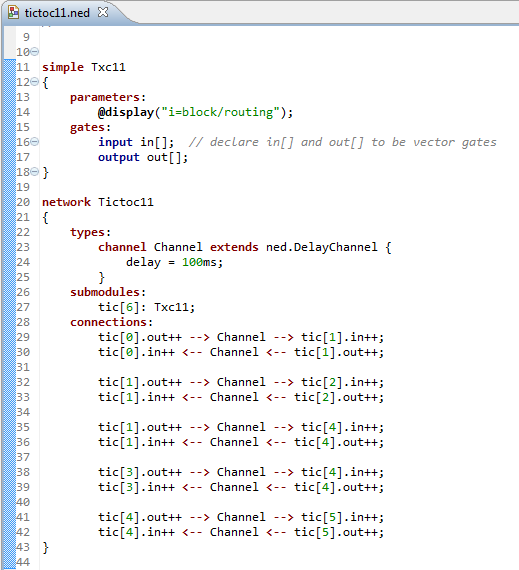
\includegraphics[width=0.52\textwidth, keepaspectratio]{Images/omnet/tictoc_ned_02}
	}
	\caption{Esempio di file NED.}
	\label{fig:ned_file}
\end{figure}
\bigskip

\subsubsection{Raccolta Dati}
OMNeT++ fornisce metodi per la raccolta di dati e statistiche e la possibilità di analizzarli al termine della simulazione. Si possono raccogliere due categorie di dati: i log temporali, chiamati anche event-log e i dati relativi a statistiche. I log temporali non sono altro che rappresentazioni grafiche della successione degli eventi tra i nodi della rete. Molto utile per analizzare la sequenza temporale degli eventi, la loro durata e le loro interazioni, soprattutto quando si hanno parecchi eventi che avvengono in contemporanea; in figura \ref{fig:elog_02} è riportato uno frammento di un event-log. Per quanto riguarda le statistiche, si possono raccogliere dati con riferimento temporale, chiamati vettori, oppure statistiche su dati, chiamati scalari, quali media, varianza, deviazione standard, somma, minimo, massimo e altri ancora. Sia sui vettori che sugli scalari è possibile poi fare delle operazioni di manipolazione dati, come eseguire raggruppamenti, applicare filtri, applicare operazioni ai dati o a gruppi di dati come l'operatore media. Si può applicare l'operatore media a un grafico temporale di vettori, per ottenere l'andamento medio, utile per visualizzare il comportamento asintotico del sistema; in figura \ref{fig:esempio_anf_01} è riportato un esempio. In figura \ref{fig:esempio_anf_grafico_01} è riportato un esempio di rappresentazione grafica di vettori temporali più la rappresentazione dell'andamento medio. In figura \ref{fig:tictoc_scalar_01} invece è riportato un esempio di istogramma come rappresentazione della distribuzione del conteggio di hop necessari per raggiungere hostess destinatario.

\begin{figure}[t]
	\centering
	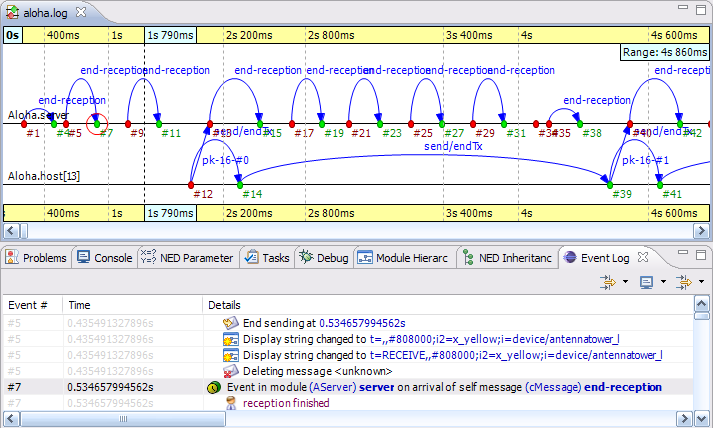
\includegraphics[width=0.7\linewidth]{Images/omnet/elog_02}
	\caption[anf file]{Esempio di event-log.}
	\label{fig:elog_02}
\end{figure}
\bigskip
\begin{figure}[tbh]
	\centering
	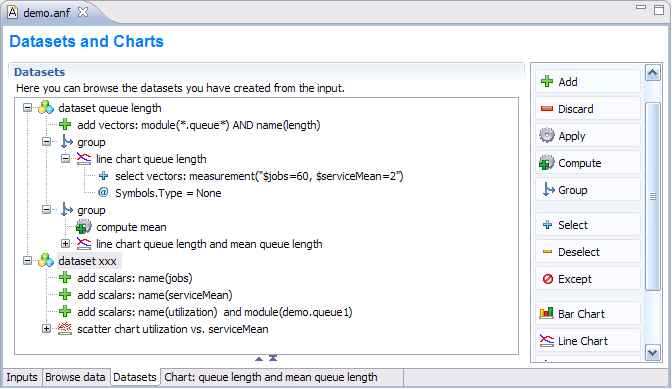
\includegraphics[width=0.7\linewidth]{Images/omnet/esempio_anf_01}
	\caption[anf file]{Esempio di manipolazione dati.}
	\label{fig:esempio_anf_01}
\end{figure}
\bigskip
\begin{figure}[tbh]
	\centering
	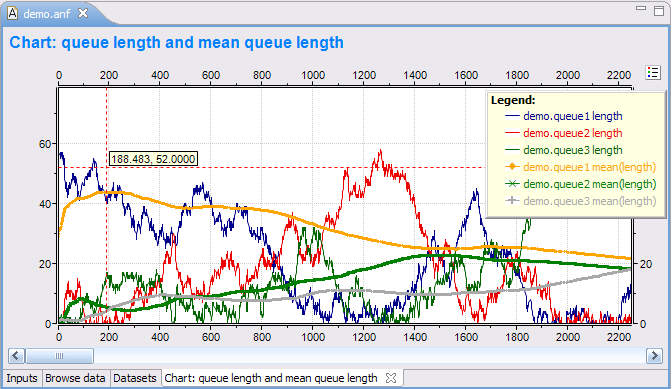
\includegraphics[width=0.7\linewidth]{Images/omnet/esempio_anf_grafico_01}
	\caption[anf file]{Esempio di grafico temporale di vettori e medie.}
	\label{fig:esempio_anf_grafico_01}
\end{figure}
\bigskip
\begin{figure}[tbh]
	\centering
	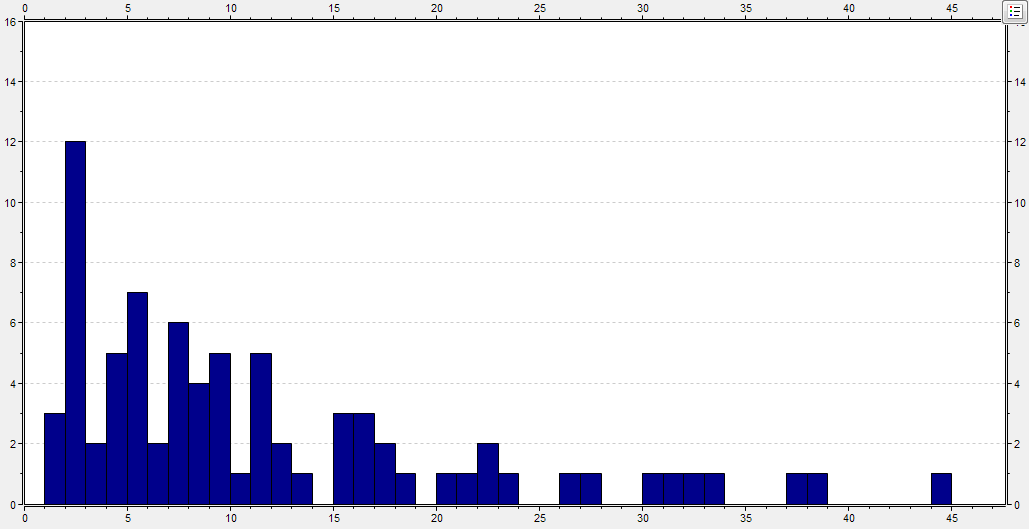
\includegraphics[width=0.7\linewidth]{Images/omnet/tictoc_scalar_01}
	\caption[anf file]{Esempio di istogramma, grafico per dati scalari.}
	\label{fig:tictoc_scalar_01}
\end{figure}
	\chapter{Impostazione del problema di ricerca}
\label{chap:impost_prob_ricerca}
	\chapter{Progettazione logica della soluzione proposta}
\label{chap:Prog_log_sol}

Dopo che lo studio sul consumo energetico, esposto nella \MySec{sec:studio_energetico}, ci ha confermato che il basso livello di energia richiesto dalla tecnologia BLE per la trasmissione di informazioni è molto limitato, ci siamo dedicati allo studio di un modello di rete che potesse descrivere correttamente la disposizione dei dispositivi e del mezzo di comunicazione. Il BLE, ma la tecnologia Bluetooth in generale, è un sistema di comunicazione molto legato alla potenza del trasmettitore e dalla relativa distanza che tale potenza consente di raggiungere. Per questo motivo abbiamo scelto di modellare la nostra rete di dispositivi mobili con una Random Geometric Graph, presentata nella \MySec{subsec:modelli_rete}. La scelta di questo modello di rete è stata abbastanza naturale, visto la comune caratteristica che di distanza fisica che accomuna la trasmissione \acs{BT} e il modello di rete stesso.

Infine dopo l'aspetto del modello di rete, ci siamo dedicati allo studio di un sistema di regole che potessero governare la diffusione delle informazioni. Dopo un'attenta analisi è emerso che per com'è composta la rete e per il tipo d'informazioni, un modo efficace di diffondere informazioni è quello del passa parola. Per questo motivo abbiamo preso in considerazione il mondo degli algoritmi di gossip, o epidemici, creati per modellare la diffusione d'informazioni tra le persone e sui social network, o nel caso degli epidemici come si diffonde un'epidemia in una popolazione. Tra gli algoritmi di gossip, abbiamo scelto di estendere l'algoritmo del \acl{FF}, un algoritmo di gossip di tipo Rumor Mongering presentato nella \MySec{subsec:alg_p2p}. La nostra soluzione è stata progettata perché tenga in considerazione il consumo energetico che essa genera sul dispositivo. Per questo motivo abbiamo progettato il nostro algoritmo, estendendo quello già esistente, aggiungendo elementi molto dinamici. Infatti, i parametri da noi progettati, regolano l'algoritmo in modo dinamico, permettendogli di adattarsi allo stato dell'ambiente esterno e allo stato interno del dispositivo. Per stato dell'ambiente esterno intendiamo il numero di dispositivi presenti nelle vicinanze, quindi lo stato della rete attorno al dispositivo, mentre per stato interno intendiamo il livello della batteria, in modo da regolare lo “sforzo” in maniera corretta. Il nostro algoritmo cerca sempre di regolare i parametri in modo da garantire un buon compromesso tra prestazioni e consumo energetico/carico di lavoro. Dopo un'attenta analisi abbiamo deciso di progettare l'algoritmo in modo che reagisse a fronte di cambiamenti nella rete o nello stato interno del dispositivo oppure in entrambi.
\bigskip

\section{Modello di rete}
Come presentato nel \MyChap{chap:impost_prob_ricerca}, negli scenari ipotizzati si avrebbe che da una situazione in cui i dispositivi sono completamente connessi, si passi a una situazione in cui i dispositivi sono isolati.
\begin{figure}[t]
	\subfloat[Rete connessa.\label{subfig-1:rete_cellulare}]{%
		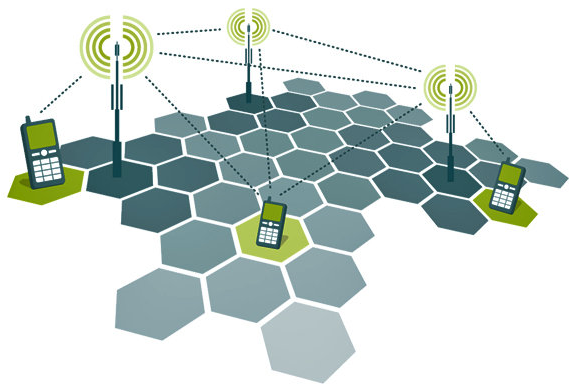
\includegraphics[width=0.45\textwidth, keepaspectratio]{Images/reti/rete_cellulare}
	}
	\hfill
	\subfloat[Rete sconnessa.\label{subfig-2:grafo_sconnesso}]{%
		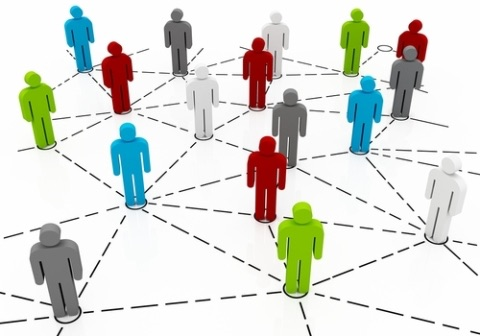
\includegraphics[width=0.45\textwidth, keepaspectratio]{Images/reti/grafo_sconnesso}
	}
	\caption{Scenari possibili.}
	\label{fig:scenari_possibili}
\end{figure}
Normalmente si avrebbe usa situazione come in \myFig{subfig-1:rete_cellulare}, dove tutti i dispositivi mobili sono connessi alla reti cellulari e la infrastruttura di comunicazione rappresenta l'overlay della rete stessa, poiché ne conosce la struttura e ne gestisce interamente le trasmissioni. Invece nelle situazioni descritte al punto tre non si hanno più questi collegamenti alla rete cellulare e ciò che rimane sono i singoli nodi senza un overlay in grado di gestirne le comunicazioni, \myFig{subfig-1:grafo_sconnesso}; l'unica possibile forma di comunicazione è una trasmissione diretta tra i nodi stessi. Dopo aver ricercato in letteratura, abbiamo capito che il modello adatto a modellare questo tipo di situazioni è quello Peer-to-Peer. Le \acs{P2P} sono reti di nodi totalmente paritetici, senza alcuna struttura gerarchica o differenziazione tra i nodi stessi. Per questo motivo ogni nodo della rete è chiamato peer e lo scambio di informazioni avviene sempre tra due peer alla volta. Tra i tanti modelli presenti in letteratura, abbiamo scelto quello che riesce a rappresentare al meglio le caratteristiche della rete da noi in esame: il modello che abbiamo scelto è il \acf{RGG}. Questo tipo di modello è costituito da un grafo \textit{G(N,$\rho$)} bidirezionale casuale inserito in un'area limitata ed è composto da N nodi. Il parametro $\rho$ rappresenta la distanza massima entro la quale sono stabiliti i collegamenti tra i nodi. Il raggio $\rho$ è di fatto la distanza geometrica entro la quale un nodo stabilisce collegamenti con altri nodi. Due nodi a una distanza inferiore di $\rho$ avranno un collegamento bidirezionale, mentre due nodi a una distanza maggiore di $\rho$ non avranno nessun collegamento tra loro. Questo tipo di modello presenta una bassa degree variance, ma un'alta edge dependency. Sono due parametri che rispettivamente indicano la varianza nella distribuzione del grado dei nodi e un fattore di dipendenza dagli archi del grafo che indica la probabilità che vi siano collegamenti tra nodi vicini.

Nel nostro caso di studio il raggio $\rho$ modella la portata del trasmettitore Bluetooth, infatti, solo dispositivi che si trovano entro il raggio d'azione dei rispettivi trasmettitori possono comunicare, mentre dispositivi fuori portata non avranno alcun collegamento. La costruzione di un \acs{RGG} inizia scegliendo le caratteristiche dell'area, base e altezza. Successivamente si dispongono in maniera casuale uniforme i nodi del grafo all'interno dell'area. Infine si controllano le distanze tra tutti i nodi e si instaurano i collegamenti solo tra i nodi a una distanza uguale o inferiore a $\rho$. In \myFig{fig:rgg_gen} sono riportati due esempi di \acs{RGG}.
\begin{figure}[t]
	\subfloat[\label{subfig-1:rgg_03}]{%
		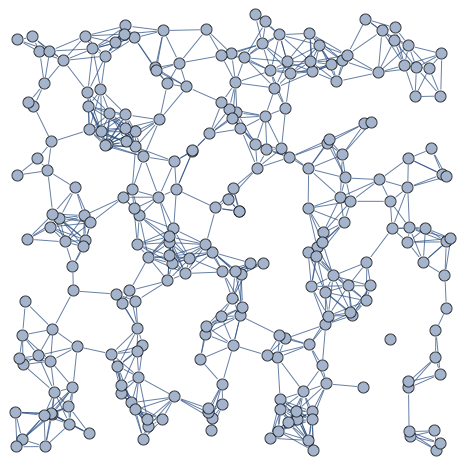
\includegraphics[width=0.48\textwidth, keepaspectratio]{Images/reti/RandomGeometricGraph_03}
	}
	\hfill
	\subfloat[\label{subfig-2:rgg_06}]{%
		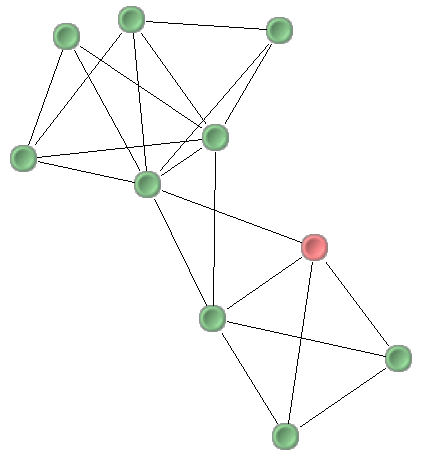
\includegraphics[width=0.42\textwidth, keepaspectratio]{Images/reti/RandomGeometricGraph_06}
	}
	\caption{Esempi di Random Geometric Graph.}
	\label{fig:rgg_gen}
\end{figure}
Com'è possibile intuire, il parametro $\rho$ è la chiave principale che determina quanto sia connesso il grafo. Più $\rho$ è piccolo più la probabilità di avere sottografi isolati e/o archi \textit{bridge} tra i sottografi è elevata. Un bridge è un arco singolo che collega un nodo di un sottografo con un nodo di un altro sottografo, rendendo quell'arco l'unica possibile via di comunicazione tra i due sottografi. Un raggio ridotto, diminuisce la possibilità di avere collegamenti ridondanti per la diffusione dell'informazione e aumenta la possibilità di avere gruppi di nodi isolati e la formazione di bottleneck nella rete. Al contrario, più il raggio cresce più la probabilità di avere nodi o sottogruppi di nodi isolati diminuisce, come anche la probabilità di avere archi bottleneck e la rete tenderà a essere sempre più connessa. Va detto anche che oltre al raggio $\rho$, è altrettanto importante la dimensione dell'area in cui la rete si trova. Nonostante l'area non sia un parametro del grafo, essa influisce, insieme a $\rho$, a rendere il grafo più o meno connesso. Il motivo è dovuto al metodo con cui è generato il grafo. Presa un'area, i nodi vengono distribuiti in modo casuale e uniforme all'interno dell'area. Più l'area è grande, più la distribuzione uniforme tenderà a disperdere i nodi. Dato un grafo con N e $\rho$ fissati, più l'area è grande più la densità dei nodi per metro quadro sarà bassa, mentre al contrario, più l'area è piccola più la densità sarà elevata. Questo fattore di dispersione ci ha permesso di poter simulare scenari diversi, dal grosso centro urbano con alta densità abitativa, fino al paese di campagna dove la popolazione è molto più diradata. Per questo motivo, è stato importante lavorare secondo ipotesi di diverse densità di nodi; fissati densità e numero di nodi, l'area è calcolata di conseguenza. Come già detto in precedenza, il nostro algoritmo presenta una componente dinamica, che tiene in considerazione le variazioni dell'ambiente esterno. Negli scenari da noi considerati, è molto facile che la densità di popolazione possa variare e per questo motivo abbiamo implementato moduli specifici che hanno lo scopo di seguire questi cambiamenti.

\section{Sistema di trasmissione}
Per le motivazioni presentate nel \MyChap{chap:impost_prob_ricerca} e perché questo sistema di trasmissione è indipendente dalle reti di comunicazione cellulare, abbiamo scelto di utilizzare il Bluetooth Low Energy come mezzo di comunicazione.

Richiamiamo brevemente la macchina a stati che rappresenta il funzionamento del Link Layer del \acs{BLE}. Essa è composta dai seguenti cinque stati:
\begin{itemize}
	\item \textbf{Standby}: stato raggiungibile da tutti gli altri stati. In questo stato non è possibile effettuare nessuna trasmissione di pacchetti né riceverne.
	\item \textbf{Advertising}: un dispositivo in questo stato si chiama advertiser e può inviare pacchetti di advertiser. Resta in ascolto per pacchetti in risposta ai suoi pacchetti di advertisinge.
	\item \textbf{Scanning}: un dispositivo in questo stato si chiama scannar e ricompre il ruolo di osservatore. Rimane in ascolto per pacchetti di advertising.
	\item \textbf{Initiating}: stato raggiungibile da tutti gli altri stati. In questo stato non è possibile effettuare nessuna trasmissione di pacchetti né riceverne.
	\item \textbf{Standby}: un dispositivo in questo stato si chiama initiator e rimane in ascolto di pacchetti di advertising. Risponderà a quei pacchetti di advertising ai quali è interessato, con un pacchetto di \textit{connection request} con l'intenzione di aprire una connessione.
	\item \textbf{Connection}: lo stato di Connection può essere raggiunto sia dallo stato di Advertising sia dallo stato di Initiating. Indica che il dispositivo sta tentando di connettersi o è connesso con un altro dispositivo. Lo stato Connection si suddivide in due ruoli: Slave e Master.
	\begin{itemize}
		\item \textbf{Slave}: il ruolo di Slave è affidato a chi arriva nello stato di Connection dallo stato di Advertising. Utilizza i parametri di connessione decisi/inviategli dal Master.
		\item \textbf{Master}: il ruolo di Master è affidato a chi arriva nello stato di Connection dallo stato di Initiator. Un dispositivo Master decide i parametri della connessione, che invierà allo Slave.
	\end{itemize}
\end{itemize}
Nell'implementazione della nostra soluzione abbiamo mappato uno a uno gli stati del \acs{BLE} con gli stati dell'algoritmo di gossip scelto, che descriveremo nella sezione successiva, in modo da avere una corrispondenza tra stato di trasmissione con stato di contagio.
In \myFig{fig:bt_fsa2} richiamiamo la macchina a stati del BLE.
\begin{figure}[tb]
	\centering
	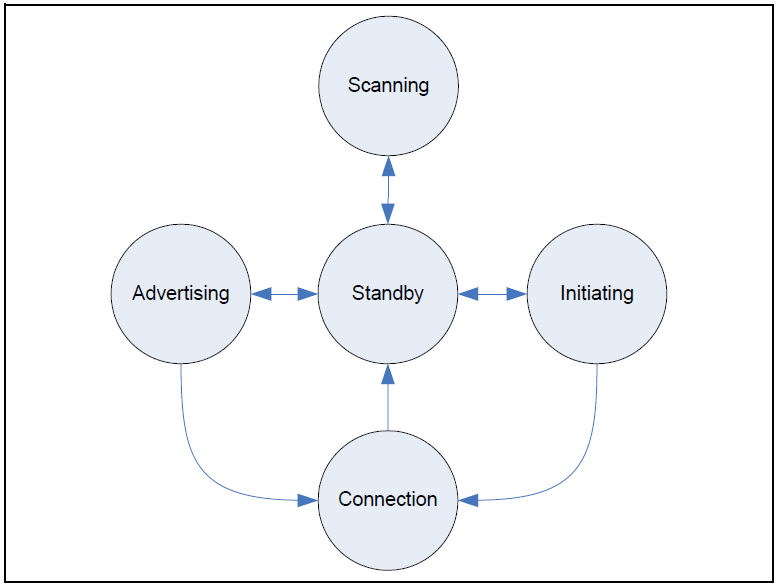
\includegraphics[width=0.8\linewidth]{Images/bt/bt_fsa}
	\caption[ble fsa]{Macchina a stati del Link Layer del BLE.}
	\label{fig:bt_fsa2}
\end{figure}
\bigskip

\section{Soluzione: Algoritmo Dynamic Fanout}
Dopo una profonda analisi degli algoritmi di gossip presenti in letteratura e della loro classificazione, abbiamo deciso di basare la nostra soluzione su algoritmi di tipo Rumor Mongering, in altre parole algoritmi che hanno come obiettivo la diffusione di un “rumore” o pettegolezzo, nel nostro caso un'informazione. Nella \MySec{subsec:alg_p2p} abbiamo presentato alcuni algoritmi di gossip adatti a reti \acs{P2P} e i diversi aspetti che li caratterizzano. La nostra scelta è stata di usare come base l'algoritmo del Fixed Fanout, per poi estenderlo con l'aggiunta di parametri dinamici, allo scopo di dare appunto dinamicità all'algoritmo e capacità di adattamento ai diversi cambiamenti dell'ambiente esterno e dello stato interno dei dispositivi stessi. Con cambiamenti dell'ambiente esterno intendiamo le variazioni della rete nel raggio d'azione del nodo, quindi il variare del numero di nodi che esso percepisce, mentre con variazioni interne al dispositivo intendiamo la variazione nel livello di carica della batteria. Questo perché abbiamo cercato di progettare i parametri in modo che abbiano sempre un valore che possa garantire prestazioni accettabili e che calibri il carico di lavoro del dispositivo in relazione al livello energetico che la batteria ha. Se il livello di energia è elevato, l'algoritmo cerca di assegnare al dispositivo un carico di lavoro maggiore se necessario, mentre se il livello di energia è medio basso, l'algoritmo comincia a calibrare i parametri in modo da trovare un compromesso di carico di lavoro ed efficienza in modo da non gravare molto sulla restante poca autonomia del dispositivo. Dato che il sistema non è né un sistema dedicato né occupa completamente le risorse di calcolo del dispositivo, non vogliamo privare l'utente degli eventuali altri servizi presenti sul suo smartphone che possano servirgli. Per questo motivo l'algoritmo, dopo che la batteria scende sotto una certa soglia limite, pone il sistema in stato di Standby per non intaccare l'autonomia residua del dispositivo.

Brevemente richiamiamo le caratteristiche dell'algoritmo di Fixed Fanout. E' un algoritmo di gossip di Rumor Mongering di tipo \acf{SIR} , con criterio di terminazione di tipo “counter”. Questo significa che nel momento di inviare una nuova informazione, l'algoritmo sceglie un nodo casuale dall'insieme dei suoi vicini e tenta di trasferirgli l'informazione. Se il trasferimento va a buon fine, incrementa un contatore di uno. Ripete quest'operazione fino a quanto il conteggio raggiunge un valore limite chiamato \textit{fanout}. Il sistema esegue esattamente \textit{fanout} trasferimenti e poi passa in stato di Rimosso. Non vi è nessun elemento di controllo su cambiamenti della rete, né vi sono elementi in grado di variare il valore di \textit{fanout}. La nostra estensione riguarda principalmente due parametri che hanno lo scopo di sostituire le componenti statiche dell'algoritmo originale con componenti dinamiche. La nostra soluzione rimane un algoritmo di tipo \acs{SIR}, ma con l'aggiunta di controlli finalizzati alla riduzione dello spreco energetico. Nell'implementazione del nostro algoritmo, abbiamo associato a ogni stato dell'automa del Link Layer del BLE uno stato del paradigma SIR. Il mapping è il seguente:
\begin{itemize}
	\item Suscettibile $ \longleftrightarrow $ Initiating.
	\item Contagiato $ \longleftrightarrow $ Advertising.
	\item Rimosso $ \longleftrightarrow $ Standby.
\end{itemize}
Questa è l'associazione teorica generale, relativa alla generica informazione. All'atto pratico, si aggiungono allo stato di Rimosso anche gli stati di Initiating e di Scanning, perché quando un dispositivo perde interesse a diffondere un'informazione, esso può anche entrare in stato di Initiating alla ricerca o in attesa di nuove informazioni da condividere, oppure passare in stato di Scanning se vuole solo ascoltare la rete passivamente.

I parametri che abbiamo progettato rappresentano due diversi criteri di terminazione: uno di tipo counter e uno di tipo blind. In questo modo il sistema ha controlli sia esterni che interni. I parametri in questione sono:
\begin{itemize}
	\item Dynamic Fanout.
	\item Advertising Limit.
\end{itemize}
%Il Dynamic Fanout ha la stessa funzione del precedente \textit{fanout}, rappresentare il limite di trasmissioni che il dispositivo può compiere. Nel nostro algoritmo però, il Dynamic Fanout viene calcolato dinamicamente e tenuto aggiornato in maniera periodica.
Il Dynamic Fanout rappresenta il limite alle trasmissioni, mentre l'Advertising Limit rappresenta il limite agli Advertising Event a vuoto consecutivi.
%L'Advertising Limit è un nuovo parametro di terminazione, introdotto e progettato allo scopo di far capire al dispositivo, quale sia la situazione della rete attorno a lui in termini di contagio. Serve a segnalare al nodo quando i nodi attorno a lui non sono più interessati alla sua informazione. Anche l'Advertising Limit è aggiornato periodicamente.

\subsection{\acf{DF}}
Il \acf{DF} ha la stessa funzione del precedente \textit{fanout}, rappresentare il limite di trasmissioni che il dispositivo può compiere. Nel nostro algoritmo però, il \acs{DF} è calcolato dinamicamente e tenuto aggiornato in maniera periodica. Nell'algoritmo di \acs{FF}, il dispositivo continua a tentare a trasmettere l'informazione finché raggiunge il limite fissato di \textit{fanout}. Nella nostra soluzione invece, il dispositivo prova a trasmettere fino a \acs{DF} volte, ma non vi è obbligato perché vi sono altri controlli in grado di stabilire quando fermare la diffusione perché il sistema ha rilevato inutile continuare. Questo controllo coinvolge l'Advertising Limit. Il DF è composto di due fattori, uno che tiene conto del livello della batteria (parte Blind) e uno che tiene conto dello stato della rete attorno al dispositivo quindi il numero di nodi percepiti (limite per il Counter). Il componente che tiene conto della batteria rappresenta un fattore di partizionamento che sarà usato per scegliere il limite di trasmissioni a seconda di quanti nodi il dispositivo percepisce. Ad esempio, se il sistema ha la batteria totalmente carica, il fattore di partizionamento sarà del 50\%, mentre se la batteria è meno della metà, sarà ad esempio del 20\%. Nel capitolo successivo, esporremo più nel dettaglio come questo parametro è calcolato e come si caratterizza l'andamento dinamico.

\subsection{\acf{AL}}
L'\acf{AL} è un nuovo parametro di terminazione, introdotto e progettato allo scopo di far capire al dispositivo, quale sia la situazione della rete attorno a lui in termini di contagi. Questo parametro rappresenta il limite di pacchetti di advertising che possono andare a vuoto consecutivamente. Quando un nodo riceve una nuova informazione da condividere, esso inizia le trasmissioni e comincia a inviare l'informazione ad altri nodi, uno alla volta. Al termine di ogni trasmissione, se il limite DF non è ancora stato raggiunto, il nodo inizierà a inviare nuovamente pacchetti di advertising alla ricerca di altri nodi ancora da contagiare. Il sistema, tramite l'uso di timeout, capisce quando un pacchetto di advertising va a vuoto e, nel caso, ne invia un altro. Allo stesso tempo conteggia il numero di pacchetti di advertising che vanno a vuoto consecutivamente. Se questo conteggio raggiunte l'AL, il nodo si ferma e passa in stato di Rimosso o di Initiating per le motivazioni sopra dette, esattamente come se avesse effettuato tutte le DF transazioni. Lo scopo principale di questo parametro è di intervenire dove il controllo DF è cieco, cioè nel controllare se tra i dispositivi che il sistema percepisce, c'è qualcuno realmente interessato all'informazione. Potrebbe accadere che la rete cambi proprio dopo aver aggiornato i parametri e quindi un dispositivo si ritroverebbe con un DF grande e non coerente con il reale stato della rete, fino al prossimo aggiornamento. In queste situazioni l'AL entra in gioco e impedisce al dispositivo di sprecare batteria, qualora l'AL sia raggiunto.
Come il DF anche l'AL è composto di un fattore per il livello della batteria e di un fattore riguardante lo stato della rete circostante il nodo. Come sarà poi spiegato nel capitolo successivo, il fattore riguardante la batteria è stato tenuto neutro, poiché l'energia richiesta per fare advertising è molto esigua e quindi abbiamo deciso di usare un fattore di partizionamento neutro; la funzione inserita per il fattore relativo ai nodi percepiti è sufficientemente restrittiva.

\section{Simulazione}
Durante la fase di studio e progettazione iniziale, abbiamo analizzato diversi sistemi e piattaforme di simulazione in grado di simulare reti come quella da noi studiata. Si faccia riferimento alla \MySec{sec:simulatori} per la presentazione generale. La nostra scelta è ricaduta su OMNeT++, un framework e libreria di simulazione basata sul linguaggio C++, estendibile e modulare. OMNeT++ è un software di simulazione molto diffuso sia nel settore commerciale sia nel settore scientifico per la simulazione di reti e protocolli di trasmissione. OMNeT++ è un software che offre un editor di sviluppo basato su Eclipse. Sono disponibili una gran varietà di strutture base come reti wired e wireless ed è possibile aggiungere estensioni che permettono di ampliare la gamma di reti supportate. INET è una delle estensioni più corpose del framework e contiene una grossa quantità di reti e protocolli delle più diffuse strutture di rete utilizzate.

Lo sviluppo anche in ambito commerciale ha reso questo strumento molto ricco di funzionalità e strumenti e anche di componenti di simulazione. OMNeT++ è fornito di un motore di simulazione event based ma come spiegato anche nella Sezione 2.5, è in grado di gestire anche azioni cicliche. Grazie al suo tool grafico Tkenv, è possibile visualizzare con animazioni la rete e i pacchetti in movimento in essa; vi è anche la possibilità di modificare alcuni aspetti visivi su Tkenv, tramite apposite istruzioni, per avere a runtime maggior espressività e potenzialità della simulazione stessa. OMNeT++ permette anche un'ottima gestione della parte di layout della rete tramite il suo linguaggio di alto livello chiamato \acf{NED}, che permette di esprimere la struttura della rete in modo semplice e permette anche l'utilizzo di funzioni di casualità, così da poter creare una rete casuale. Il generatore di numeri casuali, per permettere di poter ripetere una simulazione nelle stesse condizioni, utilizza sempre gli stessi seed. Ciò significa che la disposizione causale che si ottiene eseguendo la simulazione, sarà uguale alla disposizione ottenuta eseguendo nuovamente la simulazione da capo una volta terminata la prima. Per ottenere diverse strutture causali è necessario dire al simulatore di fare più simulazioni data la configurazione. OMNeT++ poi, necessità l'implementazione di almeno un file di configurazione nel quale specificare tutte le configurazioni di simulazione e i valori dei parametri che la simulazione richiede. Anche in questo caso è possibile utilizzare funzioni casuali messe a disposizione dal sistema per assegnare valori ai parametri. Infine OMNeT++ ha già un sistema interno per la raccolta dati e l'analisi di statistiche fatte sui dati raccolti. Permette anche di visualizzare i dati raccolti e le eventuali statistiche su grafici. Inoltre permette anche di eseguire manipolazioni sui dati raccolti, come la possibilità di raggruppare dati, eseguire operazioni di media o varianza e tante altre; è possibile inoltre per l'utente specificare particolari operazioni tramite l'apposita sintassi del simulatore. Nel \MyChap{chap:architettura} verranno illustrati più in dettaglio gli aspetti riguardanti l'utilizzo dei file di Network Definition, dei file di configurazione e delle loro caratteristiche.
	\chapter{Architettura del sistema}
\label{chap:architettura}

\section{Modello di rete}
\label{sec:modello_rete}
Il modello di rete utilizzato è quello del \acf{RGG}, una rete di nodi rappresentata da un grafo connesso. I nodi sono connessi tra loro utilizzando il criterio di distanza geometrica, quindi ogni nodo sarà collegato con tutti quei nodi che sono ad una distanza uguale o inferiore di un dato raggio $\rho$ da essi. Il raggio $\rho$ sarà una variabile del nostro problema. Nella figura 5.1 sono rappresentati due esempi di \acs{RGG}; la \myFig{subfig-2:rgg_06_bis} è un esempio di rete \acs{RGG} rappresentata dal tool grafico Tkenv di OMNeT++.
\medskip

\begin{flushleft}
	La generazione della nostra rete dipende da:
\end{flushleft}
\begin{itemize}
	\item Densità dei nodi.
	\item Numero di nodi che compongono la rete.
	\item Raggio d'azione del \acs{BLE} (\textit{$\rho$}).
\end{itemize}
La scelta di operare a diversi livelli di densità è dovuta al fatto di aver voluto studiare il comportamento della nostra soluzione in alcuni scenari urbani possibili per diverse distribuzioni geografiche sul territorio, in altre parole poter studiare il variare del comportamento del nostro algoritmo sia in situazioni di centri urbani normalmente molto densamente popolati, ad esempio medie/grandi città, sia in centri urbani con una più bassa concentrazione urbana che rappresentano la maggioranza dei paesi italiani.
Per queste considerazioni, abbiamo ipotizzato di associare al singolo nodo un abitante, perché mediamente ogni persona possiede uno smartphone, come riportato anche dai dati presentati dall'ISTAT \cite{istat2014}. Abbiamo scelto come prima e più grande densità 0.02 abitanti per metro quadro perché ci è sembrato una densità già sufficientemente alta per avere ottimi valori in termini di perfomance, quindi scegliere densità superiori non ci è sembrato utile per il nostro scopo. Quello che invece abbiamo voluto studiare è come si degradano le prestazioni al diradarsi della concentrazione urbana, ed ecco il perché della scelta delle alte densità.
\bigskip
\begin{figure}[t]
	\subfloat[\label{subfig-1:rgg_03_bis}]{%
		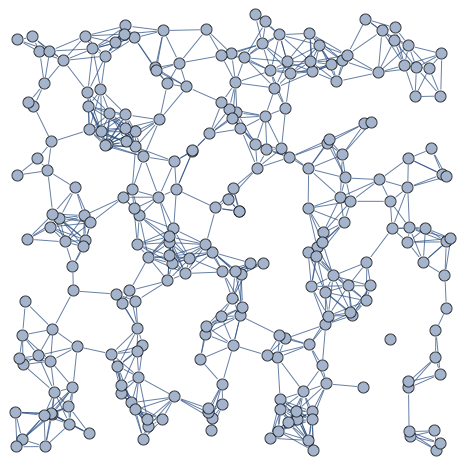
\includegraphics[width=0.45\textwidth, keepaspectratio]{Images/reti/RandomGeometricGraph_03}
	}
	\hfill
	\subfloat[\label{subfig-2:rgg_06_bis}]{%
		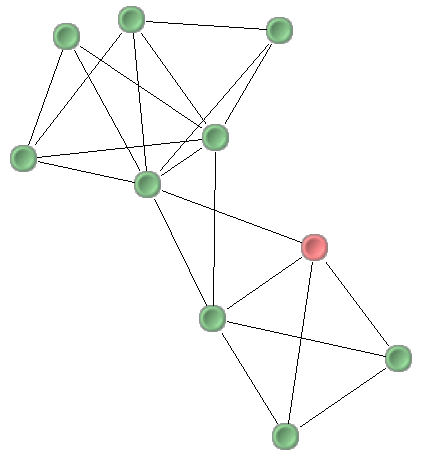
\includegraphics[width=0.45\textwidth, keepaspectratio]{Images/reti/RandomGeometricGraph_06}
	}
	\caption{Esempio di file di inizializzazione.}
	\label{fig:rgg_gen_02}
\end{figure}
\bigskip

\noindent{Le densità scelte sono:}
\begin{itemize}
	\item d = 0.02 $ \dfrac{nodi}{m^{2}} $.
	\item d = 0.01 $ \dfrac{nodi}{m^{2}} $.
	\item d = 0.008 $ \dfrac{nodi}{m^{2}} $.
	\item d = 0.001 $ \dfrac{nodi}{m^{2}} $.
	\item d = 0.0005 $ \dfrac{nodi}{m^{2}} $.
	\item d = 0.0001 $ \dfrac{nodi}{m^{2}} $.
\end{itemize}
La generazione dell'area dipende anche dal numero di nodi in quanto, per mantenere un certo valore di densità è necessario che il rapporto tra il numero di utenti e l'area analizzata sia corretto. Quindi per ogni densità abbiamo scelto di fare molteplici prove con diversi valori di utenti. I valori di N che vanno da 2 a 100, sono valori pensati per simulare situazioni reali, mentre i valori più grandi sono stati scelti per vedere la scalabilità della nostra selezione in casi estremi.
\medskip

\noindent{I valori per il numero di nodi scelti sono:}
\begin{itemize}
	\item N = 2.
	\item N = 5.
	\item N = 10.
	\item N = 30.
	\item N = 50.
	\item N = 80.
	\item N = 100.
	\item N = 200.
	\item N = 500.
	\item N = 1000.
\end{itemize}
Come già anticipato, una volta fissata la densità e il numero di nodi si ricavano le misure dell'area in analisi. Abbiamo scelto di operare in questo modo perché scegliere direttamente la grandezza dell'area senza vincoli, avrebbe portato alla scelta di aree troppo piccole o troppo grandi. Un area troppo piccola per il numero di nodi ha come conseguenza di presentare prestazioni perfette sempre, mentre scegliere un'area troppo grande restituirebbe la non utilità del sistema, a causa della troppa dispersione spaziale dei nodi. Scenari di questo tipo non sono oggetto delle nostre analisi.

Infine l'ultimo parametro che abbiamo voluto far variare è stato il raggio d'azione $\rho$ del BLE. Le specifiche tecniche non danno nessuna indicazione della distanza coperta da questa tecnologia, perché, rispetto al precedente BT Classic, la scelta di questo fattore viene delegato alle aziende produttrici dei trasmettitori. La distanza dipende da quanto potente viene costruito un trasmettitore.
Lo studio \cite{tesi_tibertoa2013} ha stimato che in media la distanza è di 50 m, ma altri studi hanno rilevato che si può arrivare anche ad oltre 100 m in linea d'aria. Per il nostro caso di studi, poiché i dispositivi in analisi sono dispositivi mobili come smarthphone e tablet, abbiamo scelto di prendere un valore pessimistico e uno ottimistico. Questo perché, i trasmettitori equipaggiati sui dispositivi mobili non sono tutti uguali e quindi la scelta di studiare due valori agli estremi ci è parsa logica.
\medskip
\noindent{I valori di $ \rho $ scelti sono:}
\begin{itemize}
	\item $\rho$ = 15 m.
	\item $\rho$ = 50 m.
\end{itemize}
Abbiamo scelto di utilizzare come valore più piccolo, un raggio poco più grande di quello della Classe 2 del Bluetooth Classic, che è di norma la distanza raggiunta dai dispositivi cellulari precedenti gli smartphone. Come termine massimo invece, abbiamo scelto di utilizzare il valore medio stimato dallo studio \cite{tesi_tibertoa2013}. Ci è sembrato sensato che un normale smartphone non vada oltre i 50 m per un motivo: gli smartphone e i tablet sono soggetti ad una progettazione minimalista che cerca di compattare il più possibile in pochi millimetri di spessore. Questo comporta ad installare trasmettitori di potenza sufficiente per coprire l'utilizzo dei componenti accessori che il mercato offre (dispositivi wearable) e che possano occupare lo spazio desiderato dai designer, a differenza dei trasmettitori progettati per applicazioni in ambito industriale, i quali devono coprire distanze anche superiori a 100 m a volte, vengono progettati con l'obiettivo primario della distanza, senza vincoli di volume.

\subsection{Costruzione della rete}
In fase di simulazione, la generazione della rete viene fatta in modo automatico dal simulatore come la distribuzione dei nodi nell'area e la costruzione dei collegamenti tra i nodi. I vari parametri necessari, grandezza dell'area, numero dei nodi e raggio $\rho$ sono inseriti negli appositi file d'inizializzazione. Quando viene eseguito lo scrip di lancio, viene caricato il file di inizializzazione corrispondente al caso di simulazione e nel file di Network Definition vengono caricati i valori dei parametri specificati nel file di inizializzazione caricato. Il file \acs{NED} relativo al \acs{RGG}, si faccia riferimento al codice all'\MyAppendix{fig:rgg_code}, contiene i metodi per la costruzione della rete. Come prima cosa, i nodi vengono posizionati in maniera casuale e uniforme nell'area specificata, poi nella sezione \textit{connections} vi è il metodo che controlla e inserisce i collegamenti tra i nodi. Dopo aver disposto casualmente i nodi nell'area, per ogni nodo controlla quali altri nodi si trovano ad una distanza geometrica inferiore al valore di $\rho$ specificato nel file di inizializzazione e tra essi inserisce un canale di comunicazione con le prestazioni di trasmissione del BLE.

\subsection{Algoritmo Dynamic Fanout}
Come presentato nella \MySec{chap:Prog_log_sol} la nostra soluzione è una estensione dell'algoritmo di gossip Fixed Fanout (vedere \MySec{subsec:alg_p2p}). Abbiamo esteso il metodo di calcolo per il limite del numero di trasmissioni che ogni nodo può effettuare, inserendo nuove componenti dinamiche che hanno reso lo stesso fattore reattivo ai cambiamenti sia ambientali sia interni al dispositivo. Per questo motivo abbiamo chiamato il nostro algoritmo: Dynamic Fanout. Successivamente, abbiamo aggiunto un controllo per la terminazione delle trasmissioni che vengono segnalate inutili, permettendo all'algoritmo di limitare gli sprechi di energia. In questo modo il sistema cerca sempre di trovare un punto di lavoro che offra un compromesso tra efficienza e risparmio energetico nella maggior parte degli scenari studiati.

I due principali fattori che abbiamo progettato sono il Dynamic Fanout e l'Advertising Limit. Sono due parametri che rappresentano due criteri di terminazione di tipo contatore, ma che al loro interno hanno anche una componente di tipo "blind" necessaria a valutare lo stato della batteria del dispositivo. Il Dynamic Fanout rappresenta il limite di trasmissioni che il dispositivo può fare nel suo stato, mentre l'Advertising Limit rappresenta il limite di trasmissioni di advertising andate a vuoto consecutivamente che il dispositivo deve fare per decidere che nessuno dei suoi vicini è più interessato ad averla.

Il nostro algoritmo agisce basandosi sulla macchina a stati del BLE, cambiando stato all'avvenire di particolari eventi. Avendo fatto una relazione uno a uno tra gli stati dell'algoritmo di gossip e quelli della macchina a stati del BLE, abbiamo potuto centralizzare la gestione sul Bluetooth. Anche se il BLE per definizione è un sistema di trasmissione che consuma poca energia, abbiamo deciso che il nostro sistema sia in uno stato di attiva operatività finché la batteria del dispositivo è superiore al 10\%. Questo perché, non vogliamo che il sistema vada a consumare le ultime riserve di energia del dispositivo, permettendo all'utente di usufruire di tutti quei servizi sul dispositivo di cui ha bisogno e di raggiungere eventualmente una fonte di ricarica. Inoltre la maggior parte degli smartphone implementa già sistemi di risparmio energetico che disabilitano sistemi non essenziali quando la batteria scende sotto certi livelli.
Il nostro algoritmo, qualora la batteria scenda sotto il 10\%, finisce l'eventuale trasmissione in corso e poi si porta in stato di Standby. Quando la batteria torna sopra il 10\%, il sistema torna attivo e operativo. Questo controllo viene fatto periodicamente, tramite una procedura che esegue le "azioni periodiche". Sono azioni che devono essere eseguite periodicamente, indipendentemente dall'occorrenza di eventi esterni. Queste azioni periodiche prevedono il controllo dello stato della batteria e l'aggiornamento dei parametri. Questo processo rimane attivo anche quando la batteria scende sotto la soglia limite e continua i suoi aggiornamenti, così da poter riattivare subito il sistema quando la batteria viene caricata. Nel nostro caso di studio abbiamo simulato la decadenza della batteria tramite il decremento di una variabile numerica.
\begin{algorithm}[t]
	\caption{Azioni Periodiche}\label{alg:periodic_actions}
	\begin{algorithmic}[1]
		\Function{AzioniPeriodiche}{\textit{btState}}
		\State \textit{decrementaBatteriaIdle()}
		\State $ \textit{batteria} \gets \textit{livelloBatteria() } $
		\If{$\left(  \textit{busy} \: || \: \textit{batteria} \geq 0 \right) $}
		\State \textit{AggiornaParametri(\textit{batteria})}
		\If{$\textit{btState} = STANDBY $}
		\State $ \textit{btState} \gets INITIATING $
		\EndIf
		\Else
		\State $ \textit{btState} \gets STANDBY $
		\EndIf
		\EndFunction
	\end{algorithmic}
\end{algorithm}
Un decremento costante ad ogni azione periodica per simulare il normale consumo della batteria, più un consumo ad ogni trasmissione/ricezione che il dispositivo effettua, per accentuare il fatto che il consumo energetico del sistema è concentrato nelle trasmissioni e non nel suo stato di attesa. Abbiamo scelto di decrementare la batteria ad ogni azione periodica, quindi col risultato di un consumo energetico medio più alto di quello reale, per studiare come si comporta il sistema con dispositivi soggetti ad un alto consumo energetico esterno al nostro sistema. Lo pseudo codice dell'\MyAlg{alg:periodic_actions} descrive il funzionamento delle azioni periodiche, che vengono schedulate periodicamente dal sistema. La variabile booleana \textit{busy} segnala quando il dispositivo è impegnato nell'esecuzione di qualche trasmissione o ricezione. All'\MyAppendix{apx:stb_fsa}, riportiamo il diagramma di flusso della macchina a stati Standby. Questo diagramma sintetizza il comportamento del sistema nei momenti di inattività. All'avvenire di azioni periodiche, il sistema controlla il livello di batteria e se maggiore del 10\%, porta il sistema in stato di Initiating. Se il sistema riceve dall'utente il comando di inviare un messaggio, esso passa in modalità di invio di un nuovo messaggio e l'\MyAlg{alg:invia_msg} descrive in pseudo codice le operazioni necessarie.

\begin{algorithm}[ph]
	\caption{Invio Messaggio}\label{alg:invia_msg}
	\begin{algorithmic}[1]
		\Function{InvioMessaggio}{\textit{btState},\textit{msg}}
			\If{$\textit{btSt}ate \neq STANDBY$}
				\State $ \textit{btState} \gets STANDBY$
			\EndIf
		\State $ \textit{Tx counter} \gets 0 $ \Comment{Contatore trasmissioni effettuate.}
		\Label \spacedlowsmallcaps{start:}
		\State $ \textit{AE counter} \gets 0 $ \Comment{Contatore degli Advertising Event.}
		\State $ \textit{btState} \gets ADVERTISING$
		\State $ AE counter \gets +1 $
		\State \textbf{begin}
			\State\hspace{\algorithmicindent}{ADVERTISING EVENT}
		\State \textbf{end}
		\If{$\textit{èTimeoutScaduto()}$}
			\If{$ \textit{AE counter}\,<\,\textit{AL}$}\Comment{AL = Advertising Limit.}
				\State \textbf{go to} \spacedlowsmallcaps{start}
			\Else
				\State $btState \gets STANDBY$
				\State \textit{AzioniPeriodiche(btState)}
			\EndIf
		\EndIf
		\State $ \textit{busy}\gets VERO $
		\State $\textit{btState}\gets CONNECTION\_SLAVE$
		\State \textbf{begin}
			\State\hspace{\algorithmicindent}{CONNECTION EVENT}
		\State \textbf{end}
		\State $\textit{Tx counter}\gets +1$
		\State $ \textit{decrementaBatteriaTx()}$
		\State $\textit{busy}\gets FALSO$
		\State $ \textit{btState}\gets STANDBY $
		\If{$ \textit{Tx counter}\,<\,DF$}
			\State \textbf{go to} \spacedlowsmallcaps{start}
		\Else
			\State \textit{AzioniPeriodiche(btState)}
		\EndIf
		\EndFunction
	\end{algorithmic}
\end{algorithm}

All'\MyAppendix{apx:invio_fsa} riportiamo il diagramma di flusso della macchina a stati dell'\MyAlg{alg:invia_msg}.

Per inviare un messaggio, il sistema entra si porta in stato di Standby se non lo fosse già stato, inizializza le variabili contatore per \acf{AE} e Trasmissionipoi e passa in stato di Advertising. A questo punto incrementa il contatore degli \acl{AE} e inizia l'\acs{AE} vero e proprio. Dopo aver trasmetto i suoi pacchetti, si mette in attesa di una risposta. Se il timeout scatta prima che una richiesta di connessione arrivi, allora quell'AE viene considerato a vuoto. Viene quindi controllato che il nuovo di AE a vuoto non sia superiore all'AL e poi si ricomincia con un altro AE. Se invece il AE counter è maggiore o uguale dell'AL, il sistema si ferma e si riporta sulle azioni periodiche e quindi in stato di ascolto (Initiating). Se invece, prima che scada il timeout, riceve una richiesta di connessione, allora il sistema si dichiara \textit{busy}, occupato, si porta nello stato di Connection col ruolo di Slave e attende che il Connection Event cominci. Una volta terminata la trasmissione, incrementa il contatore delle trasmissioni, resetta il contatore degli Advertising Event, si dichiara non più occupato e si porta in stato di Standby. Infine il sistema controlla se ha effettuato DF transazioni. In caso negativo si riporta all'inizio di tutta la procedura, in caso positivo esce e riprende le azioni periodiche.
Se il sistema rileva la presenza di un nuovo messaggio sulla rete, esso passa in modalità di ricezione di un nuovo messaggio e l'\MyAlg{alg:ricevi_msg} descrive in pseudo codice le operazioni necessarie. All'\MyAppendix{apx:ricevi_fsa} riportiamo il diagramma di flusso della relativa macchina a stati. Il fatto di rilevare un informazione nuova presuppone che il sistema sia in nello stato di Initiating. Se il sistema sta nello stato di Initiating, automaticamente resta in ascolto di nuove informazioni. Una volta nello stato di ascolto, quando rileva una nuova informazione, il sistema manda una richiesta di connessione al mittente del pacchetto di advertising. Dopo di che si segna come occupato ed entra nello stato di Connection col ruolo di Master e invia la richiesta di apertura del Connection Event. Se il timeout scade, vuol dire che la richiesta di connessione non è stata accettata e quindi il sistema si dichiara non più occupato e si riporta in stato di ascolto. Se invece la richiesta di connessione viene accetta, alla richiesta di apertura del Connection Event segue in risposta l'informazione, così da entrare definitivamente nel Connection Event. Completata la ricezione del messaggio, esso viene salvato, il sistema si dichiara non occupato e poi inizia ad inviare a sua volta questo nuovo messaggio.
\bigskip
\begin{algorithm}[th]
	\caption{Ricevi Messaggio}\label{alg:ricevi_msg}
	\begin{algorithmic}[1]
		\Function{RiceviMessaggio}{\textit{btState}}
		\If{$\textit{btState = INITIATING}$}
			\State \textbf{go to} \spacedlowsmallcaps{send}
		\EndIf
		\Label \spacedlowsmallcaps{start:}
		\State $\textit{btState} \gets STANDBY$
		\State $\textit{btState} \gets INITIATING$
		\Label \spacedlowsmallcaps{send:}
		\State $ \textit{invioRichiestaConnessione()}$
		\State $ \textit{busy} \gets VERO$
		\State $ \textit{btState} \gets CONNECTION\_MASTER $
		\State $ \textit{inviaRichiestaPool()}$\Comment{Richiesta d'apertura di C.E.}
		\If{$\textit{èTimeoutScaduto()}$}
			\State $ \textit{busy} \gets FALSO$ \Comment{La richiesta non è stata accettata.}
			\State \textbf{go to} \spacedlowsmallcaps{start}
		\EndIf
		\State \textbf{begin}
			\State\hspace{\algorithmicindent}{$\textit{msg} \gets CONNECTION EVENT$}
		\State \textbf{end}
		\State $ \textit{decrementaBatteriaTx()} $
		\State $ \textit{busy} \gets FALSO$
		\State $ \textit{InvioMessaggio}\left(\textit{msg,btState}\right)  $
		\EndFunction
	\end{algorithmic}
\end{algorithm}
\bigskip

\subsection{\acf{DF}}
Il Dynamic Fanout ha il compito di fermare il dispositivo dopo un certo numero di trasmissioni effettuate con successo per una certa informazione. Questo valore limite è calcolato in modo dinamico, dipendente dal livello di batteria del dispositivo e dal numero di nodi che il sistema riesce a percepire, quindi al numero di nodi ai quali può potenzialmente connettersi. Abbiamo voluto che questo parametro avesse un particolare andamento e rapidità di risposta in particolari situazioni e altri andamenti per altre situazioni. A tale scopo, abbiamo provato a modellare il comportamento di questo parametro attraverso diverse funzioni ottenendo quindi comportamenti più o meno conservativi, secondo la funzione scelta.

Il calcolo del DF è composto da due fattori: un primo fattore che tiene conto del livello di batteria del dispositivo, chiamato \textit{Fattore Batteria} e da un secondo fattore dipendente dal numero di nodi, che ha la funzione di correggere l'andamento globale della funzione risultante. La nostra idea è di ottenere dal Fattore Batteria una percentuale che rappresenta la quantità di nodi, tra quelli percepiti, che il dispositivo prenderà in considerazione come suo limite di trasmissione cioè come suo DF. Più batteria un dispositivo ha più alta sarà la percentuale di nodi cui potremo trasmettere l'informazione. In \myFig{fig:DF_battery_factor} riportiamo in grafico tre funzioni batteria studiate, ognuna con un andamento diverso; esse sono rispettivamente:

\begin{equation}
	\label{eq:df_bat_radq}
	y=\dfrac{\sqrt{0,2\cdot x\,-\,1,9}}{10}
\end{equation}
\begin{equation}
	\label{eq:df_bat_ln}
	y=\dfrac{\ln\left(x\,-\,8\right) }{10}
\end{equation}
\begin{equation}
	\label{eq:df_bat_log}
	y=\dfrac{\log\left(x\,-\,8\right) }{10}
\end{equation}

\begin{figure}[tb]
	\centering
	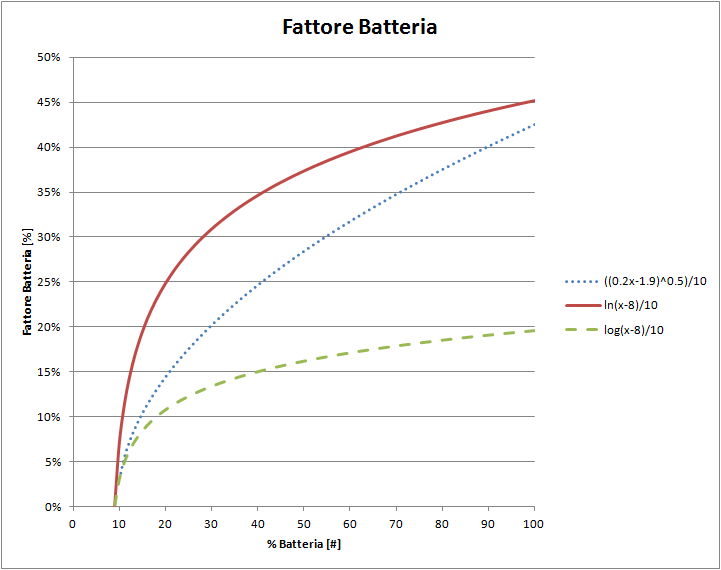
\includegraphics[width=0.9\linewidth, keepaspectratio]{Images/grafici_usati/DF_battery_factor}
	\caption[DF fattore batteria.]{Curve delle Funzioni Batteria.}
	\label{fig:DF_battery_factor}
\end{figure}
Tutte e tre le funzioni sono divise per dieci, così da ottenere un valore percentuale. Dalla \myFig{fig:DF_battery_factor} si nota come diversi tipi di funzioni diano differenti curve di risposta, più o meno conservative e più o meno reattive per valori tra 10\% e il 20\% di batteria. Noi abbiamo scelto di utilizzare la funzione di \MyEq{eq:df_bat_radq} rispetto alla funzione col logaritmo naturale, \MyEq{eq:df_bat_ln}, poiché non troppo aggressiva per valori bassi di batteria ma nemmeno eccessivamente conservativa e perché al crescere della percentuale di batteria le due funzioni tendono allo stesso valore massimo o quasi. L'\MyEq{eq:df_bat_log} risulta essere troppo conservativa e non scala bene con la crescita della rete, non permettendo una buona diffusione delle informazioni.
\medskip

\noindent{La funzione scelta per il Fattore Batteria è quindi:}
\begin{equation}
	\label{eq:df_FB}
	FB = \dfrac{\sqrt{0,2\cdot x\,-\,1,9}}{10}
\end{equation}
\begin{figure}[tb]
	\centering
	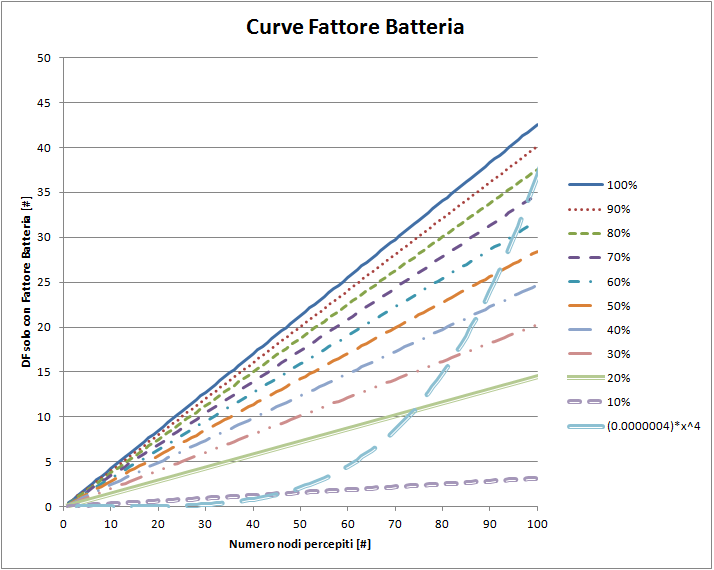
\includegraphics[width=0.9\linewidth]{Images/grafici_usati/DF_curve_fattore_batteria_corr}
	\caption[DF curve fb con correzione]{Applicazione del Fattore Batteria al numero di nodi e Fattore di Correzione.}
	\label{fig:DF_curve_fattore_batteria_corr}
\end{figure}
La variabile $\textit{x}$ rappresenta la percentuale di batteria del dispositivo ed è compresa nell'intervallo [0;100]$\in\mathbb{R}$.

Il Fattore Batteria quindi indica la percentuale sulla totalità dei nodi percepiti, da utilizzare come limite di trasmissioni. L'\MyEq{eq:df_FB} restituisce un numero valore tra 0 e 1, che applicato al numero di nodi percepiti, genera una retta linearmente crescente, al crescere del numero dei dispositivi percepiti. In \myFig{fig:DF_curve_fattore_batteria_corr} abbiamo riportato le principali rette, una ogni 10\% di batteria. Come si può notare ogni retta è monotona crescente e ciò non va bene, perché si avrebbero limiti di trasmissioni totalmente inadeguati al crescere della rete. Abbiamo quindi pensato di introdurre un fattore di correzione, che aiutasse a bilanciare la monotona crescita di queste rette. Più il numero di nodi è alto, più questo fattore correttivo è forte.

Il fattore di correzione ha la seguente equazione:
\begin{equation}
	\label{eq:df_FC}
	FC = 0.0000004x^4
\end{equation}
La variabile $\textit{x}$ rappresenta il numero di nodi percepiti dal dispositivo e $ \textit{x}\in\mathbb{R},x\geq0$

Abbiamo progettato il Fattore di Correzione in modo che possa risultare neutro per valori bassi di numero di nodi, mentre applichi la sua funzione correttiva per valori medio-grandi e grandi di numero di nodi. Questo è il motivo per cui abbiamo scelto un coefficiente così piccolo. In questo modo al crescere del numero di nodi, partendo da un valori piccoli, la componente dominante è il Fattore Batteria, poi al crescere dei nodi, la componente dominante diventa sempre più quella correttiva. Il motivo per cui abbiamo scelto di inserire questo fattore di correzione, è che ci serviva qualcosa per gestire la monotona crescita dovuta al solo fattore batteria e anche per scegliere meglio, con più criterio, il valore del DF. Col crescere della rete, cresce anche la possibilità che vi siano più dispositivi nella rete con un alto livello di batteria e quindi è possibile spalmare meglio il carico di lavoro su molti più nodi. Con una rete meno densa, lasciamo che il DF sia più grande per coprire gli eventuali dispositivi vicini che posso avere poca batteria e quindi partecipare poco o addirittura nulla al processo di diffusione. Con una rete sempre più densa invece, possiamo ridurre questo "sovraccarico", perché anche avendo la possibilità di nodi vicini con poca batteria, cresce la probabilità che vi siano altri nodi con molta batteria che possono affrontare anch'essi un buon carico di lavoro. Per questo motivo, per un alto numero di nodi, abbiamo un DF decrescente.
Unendo quindi, Fattore Batteria e Fattore correttivo abbiamo il seguente primo calcolo del DF.
\begin{align*}
	\label{eq:DF_no_asint}
	DF &= 1 \; + \; FB\cdot x \; - \; FC\\
	&= 1 \; + \left( \dfrac{\sqrt{0,2\cdot z\,-\,1,9}}{10}\; \right) \cdot x- \; 0.0000004x^4 \addtocounter{equation}{1}\tag{\theequation}
\end{align*}
La variabile $\textit{x}$ rappresenta il numero di nodi percepiti dal dispositivo e $ \textit{x}\in\mathbb{R},x\geq0$, mentre $\textit{z}$ rappresenta il livello di batteria e $\textit{z}\in \mathbb{R}, \textit{z}\in[0;100]$.

In \myFig{fig:DF_andamento_teorico} è riportato su grafico la curva del DF con l'aggiunta del Fattore di Correzione, di uno dei possibili Fattore Batteria. Ciò che si ottiene come DF è un andamento crescente come il FB fino all'intorno di $\textit{x}=50 nodi$, poi un andamento decrescente causato dall'intervento del FC. Sottolineiamo che il valore del massimo, sia in termini di valore x e valore y, varia al variare del livello di batteria. Come è facile notare dal grafico, per più di 100 nodi o per curve di batteria inferiori, il DF risulterebbe negativo. Ovviamente questo non è accettabile. Per questo motivo abbiamo anche aggiunto una componente asintotica al calcolo del DF. L'asintoto orizzontale, è pensato per stabilizzare il DF su di un valore, quando vi sono tanti nodi.
\begin{figure}
	\centering
	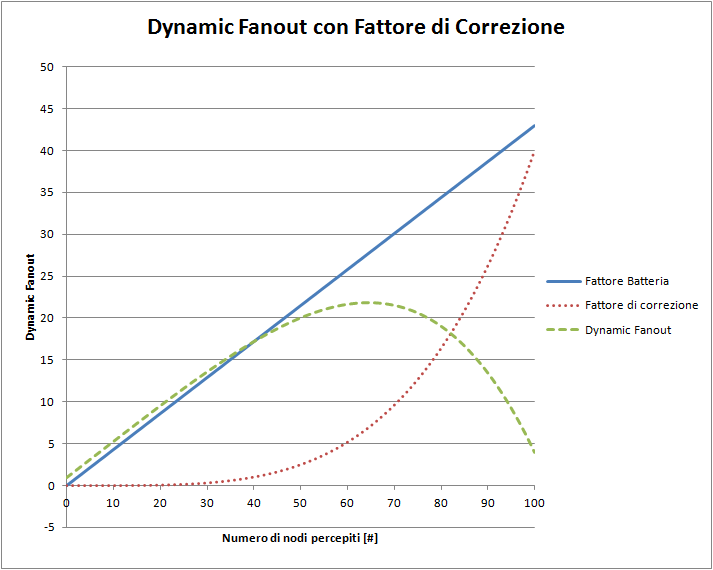
\includegraphics[width=0.9\linewidth]{Images/grafici_usati/DF_andamento_teorico}
	\caption[DF teorico]{Andamento Dynamic Fanout con correzione.}
	\label{fig:DF_andamento_teorico}
\end{figure}
La nostra scelta è basata sull'idea che oltre un certo numero di nodi, si possa trascurare la dipendenza dalla numero di nodi percepiti in quanto ci troveremmo in uno scenario di altissima densità. Quindi abbiamo pensato che è sufficiente avere un limite asintotico dipendente dal livello della batteria in modo da garantire sempre che ogni nodo non compia sforzi eccessivi consumando troppa energia. Il valore asintotico viene preso in considerazione quando il numero di nodi supera $\textit{X}_max$, quel valore di \textit{x} corrispondete al $DF_max$ per quella curva. Se $\textit{x}>\textit{X}_max$, il sistema prenderà in considerazione il valore asintotico se la curva DF con correzione è inferiore all'asintoto.
Il valore dell'asintoto è stato scelto in modo da tenere la dipendenza dal livello di batteria, così che ogni curva abbia il proprio asintoto adeguato. L'equazione dell'asintoto viene così definita:
\begin{equation}
	\label{eq:df_asintoto}
	Asintoto = 1\;+\;DF_{max}\cdot 50\%
\end{equation}
A questo punto abbiamo identificato due situazioni: $\textit{x}<\textit{X}_max$ e $\textit{x}\geq \textit{X}_max$. Unendo l'\MyEq{eq:DF_no_asint} con l'\MyEq{eq:df_asintoto} otteniamo l'\MyEq{eq:DF_totale} finale del Dynamic Fanout.
\medskip

\begin{equation}
\label{eq:DF_totale}
	\scriptsize
	DF = \begin{cases} 1 + \left( \dfrac{\sqrt{0,2\cdot z - 1,9}}{10} \right) \cdot x- 0.0000004x^4 & se\,\textit{x}<\textit{X}_{max}\\
						\max \left( 1 + \left( \dfrac{\sqrt{0,2\cdot z - 1,9}}{10} \right) \cdot x- 0.0000004x^4 ; 1 + \frac{1}{2}DF_{max} \right) & se\,\textit{x}\geq\textit{X}_{max}\end{cases}
	\normalsize
\end{equation}
In \myFig{fig:DF_tot_no_arr} riportiamo su grafico il risultato finale del calcolo del Dyanmic Fanout con asintoti orizzontali. Come prima, abbiamo rappresentato i dieci livelli di batteria.
\begin{figure}[t]
	\centering
	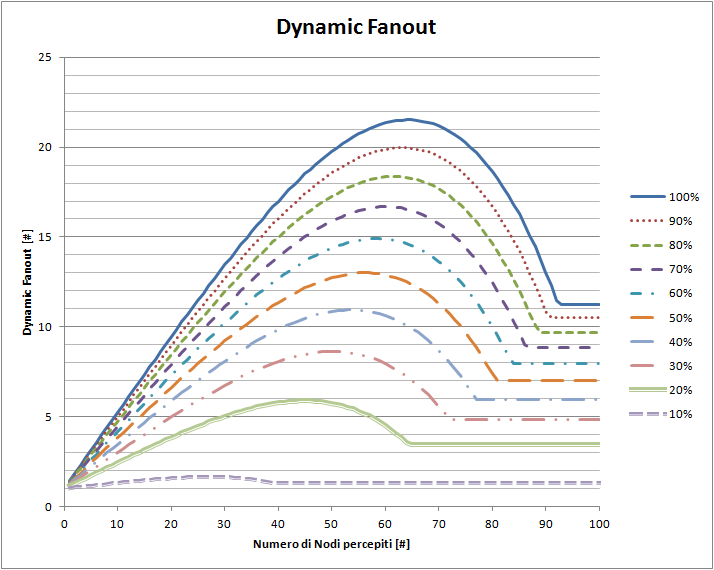
\includegraphics[width=0.9\linewidth]{Images/grafici_usati/DF_tot_no_arr}
	\caption[DF totale continuo]{Curve finali Dynamic Fanout.}
	\label{fig:DF_tot_no_arr}
\end{figure}

Dato che il DF esprime il limite di trasmissioni che un nodo può fare per ogni informazione, non ha senso avere valori non interi perché il conteggio può essere fatto solo a numeri interi. Abbiamo quindi applicato un arrotondamento per eccesso alle curve mostrate in precedenza in \myFig{fig:DF_tot_no_arr}. Il risultato è riportato in \myFig{fig:DF_tot_arr}. Applicando tale arrotondamento abbiamo ottenuto un innalzamento per tutte le curve di 1; quindi avremo il valore minimo pari a 2. Questo non crea alcun problema, anzi rende il sistema ancora più permissimo per reti piccole o diradate. Al crescere del numero di nodi percepiti, questo effetto resta trascurabile. Quello riportato in \myFig{fig:DF_tot_arr} è ciò che è stato implementato nell'algoritmo.

Abbiamo studiato anche molte altre funzioni, di vario genere e con comportamenti diversi. Alcune funzioni più conservative e altre più permissive. Di seguito riportiamo solo due casi: uno più permissivo e uno più conservativo rispetto alla soluzione scelta, con le relative formule delle funzioni utilizzate. Abbiamo riportato poi, solo i grafici finali, quelli degli andamenti totali del DF con asintoti senza arrotondamenti, per comprendere meglio le caratteristiche delle curve. Il metodo di calcolo del DF totale è lo stesso dell'\MyEq{eq:DF_totale},  cambieranno solo le funzioni che lo compongono.

\begin{figure}[t]
	\centering
	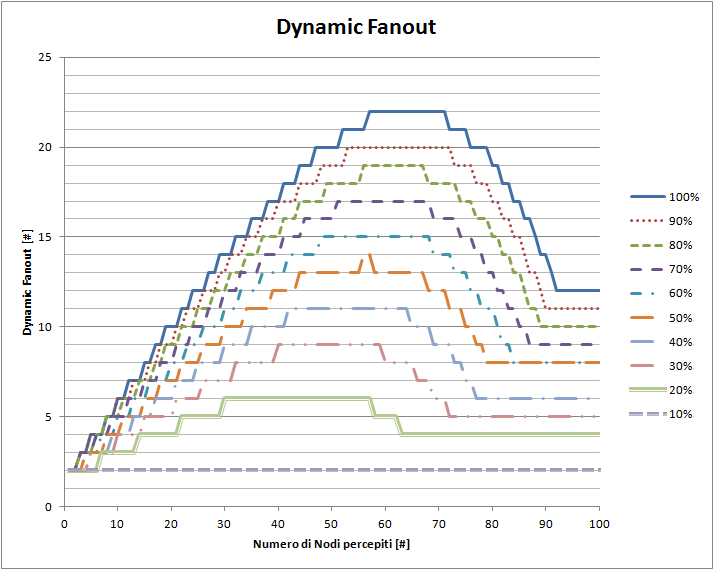
\includegraphics[width=0.9\linewidth]{Images/grafici_usati/DF_tot_arr}
	\caption[DF totale arrotondato]{Curve finali Dynamic Fanout, arrotondato per eccesso.}
	\label{fig:DF_tot_arr}
\end{figure}

Partiamo dai Fattori Batteria. Di seguito riportiamo le due funzioni in esame, più la funzione usata in soluzione, per fare meglio un confronto. Le funzioni studiate sono state molte, ma riportiamo solo quelle generate da una manipolazione della funzione utilizzata in soluzione. In \myFig{fig:DF_battery_factor_perm_conserv}, sono riportate le rispettive curve per un confronto grafico.

\begin{equation}
	\label{eq:df_bis_bat_sol}
	y=\dfrac{\sqrt{0,2\cdot x\,-\,1,9}}{10}
\end{equation}
\begin{equation}
	\label{eq:df_bis_bat_perm}
	y=\dfrac{\sqrt{0,4x}}{10}
\end{equation}
\begin{equation}
	\label{eq:df_bis_bat_cons}
	y=\dfrac{\sqrt{0,2x}}{10}
\end{equation}

L'\MyEq{eq:df_bis_bat_sol}è la stessa equazione della soluzione (\MyEq{eq:df_FB}), mentre l'\MyEq{eq:df_bis_bat_perm} e l'\MyEq{eq:df_bis_bat_cons} sono rispettivamente la funzione permissiva e la funzione conservativa.
\bigskip

\begin{figure}[tb]
	\centering
	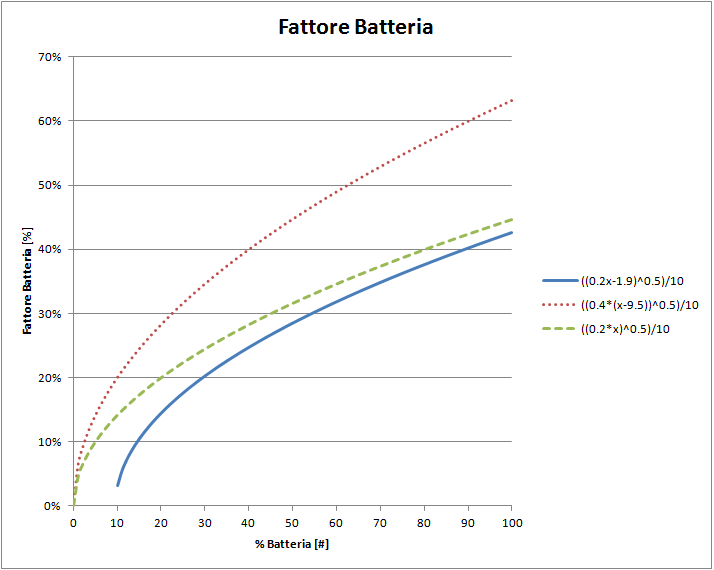
\includegraphics[width=0.9\linewidth]{Images/grafici_usati/DF_battery_factor_perm_conserv}
	\caption[Fattore Batteria bis]{Funzioni alternative per il Fattore Batteria.}
	\label{fig:DF_battery_factor_perm_conserv}
\end{figure}
\bigskip

\noindent{\textbf{\textit{{\large Caso Permissivo}}}}

Il caso permissivo nasce dalla rimozione del fattore di traslazione orizzontale e dall'incremento del coefficiente della variabile \textit{x}, da 0.2 è stato alzato a 0.4. Questo gli permette di crescere più velocemente, come si può vedere in \myFig{fig:DF_battery_factor_perm_conserv}.

Il Fattore Batteria quindi è:
\begin{equation}
	FB_{perm}=\dfrac{\sqrt{0,4x}}{10}\nonumber
\end{equation}
Aumentando il coefficiente si ottiene una crescita più ripida, quindi una reattività maggiore. Avere un fattore di partizionamento molto alto può giovare alle prestazioni, ma fino ad un certo punto perché alla fine il DF sarà così alto per ogni situazione di nodi percepiti che tale limite non sarà mai raggiunto e quindi si userà come criterio di terminazione solo l'AL, facendo diventare il DF inutile.

Il Fattore di Correzione rimane lo stesso dell'\MyEq{eq:df_FC}:
\begin{equation}
	FC = 0.0000004x^4 \nonumber
\end{equation}

L'asintoto invece è stato alzato al 70\% del DF massimo:
\begin{equation}
	\label{eq:df_asintoto_perm}
	Asintoto = DF_{max}\cdot 70\%
\end{equation}
Il calcolo del DF rimane lo stesso della soluzione descritta in precedenza. Il risultato finale lo riportiamo nel grafico in \myFig{fig:DF_permissivo_tot_no_arr}. Dal grafico si può notare che abbiamo ottenuto un incremento del valore massimo di circa 60\% o addirittura superiore, dipendente dalla curva.
\begin{figure}[t]
	\centering
	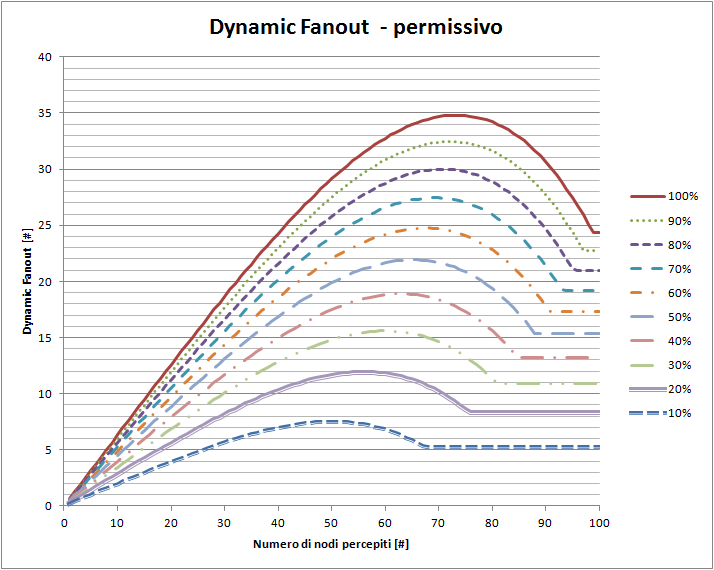
\includegraphics[width=0.9\linewidth]{Images/grafici_usati/DF_permissivo_tot_no_arr}
	\caption[DF permissivo]{Curve DF permissivo.}
	\label{fig:DF_permissivo_tot_no_arr}
\end{figure}
\bigskip

\noindent{\textbf{\textit{{\large Caso Conservativo}}}}

Per il caso conservativo, presentiamo una funzione molto simile a quella utilizzata nella soluzione, l'\MyEq{eq:df_bis_bat_cons}. E' stato rimosso il fattore di traslazione, ma il coefficiente sulle \textit{x} è rimasto lo stesso. Infatti come si può vedere nel grafico in \myFig{fig:DF_battery_factor_perm_conserv}, la funzione conservativa e quella della soluzione hanno un andamento molto simile. La principale differenza di questa versione, è di avere un Fattore di Correzione più aggressivo che agisce prima, rispetto a quello usato nelle precedenti.
\begin{equation}
	FB_{cons}=\dfrac{\sqrt{0,2x}}{10}\nonumber
\end{equation}
Il Fattore di Correzione è cambiato, il suo coefficiente è stato aumentato e il grado della funzione diminuito, per rendere tangibile la sua correzione molto prima.
\begin{equation}
	FC = 0.004x^2
\end{equation}
Anche l'asintoto è stato cambiato e scelto più basso, solo il 30\% del DF massimo delle curve.
\begin{equation}
	Asintoto = DF_{max}\cdot 30\%
\end{equation}

Il calcolo del DF è rimasto lo stesso di quello presentato precedentemente per la soluzione. Abbiamo riportato il risultato su grafico, in \myFig{fig:DF_conservativo_tot_no_arr}. Come si può notare dal grafico, abbiamo ottenuto una diminuzione del valore dei massimi da un 40\% a un 50\% rispetto alla soluzione implementata.
\begin{figure}[t]
	\centering
	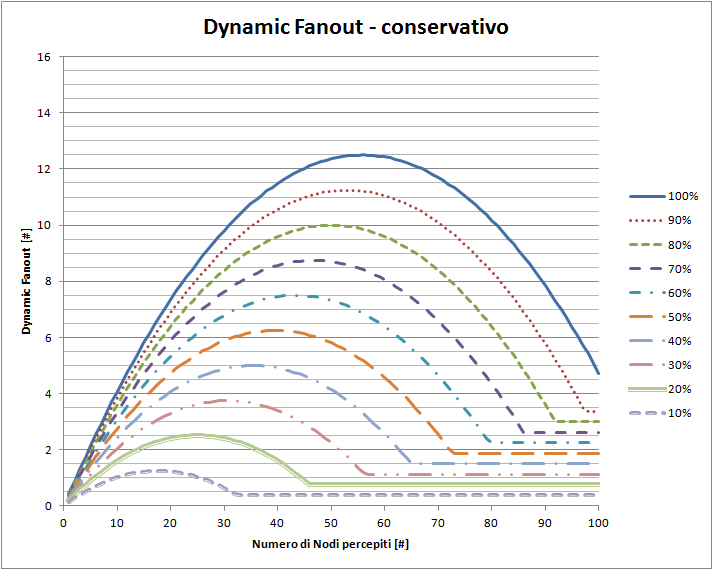
\includegraphics[width=0.9\linewidth]{Images/grafici_usati/DF_conservativo_tot_no_arr}
	\caption[DF conservativo]{Curve DF conservativo.}
	\label{fig:DF_conservativo_tot_no_arr}
\end{figure}
\bigskip


\subsection{\acf{AL}}
L'Advertising Limit ha il compito di segnalare al dispositivo quando smettere di pubblicizzare un'informazione, perché molto probabilmente è inutile e solo uno spreco di energia.  Durante la fase di advertising, vengono conteggiati gli \acf{AE} che vanno a vuoto, ovvero che non ricevono risposta. Se questo numero di advertising consecutivi senza successo diventa uguale o maggiore dell'AL, significa che con molta probabilità nessuno dei nodi vicini all'advertiser è interessato a quella informazione. A causa dei tempi di attesa imposti dalla tecnologia di trasmissione, non si può avere una certezza matematica, ma avendo inserito un ritardo tra un tentativo di advertising e il successivo, un nodo può essere sufficientemente sicuro. Nel caso un nodo prenda una decisione errata, significa che vi sono tanti nodi nelle vicinanze e quindi l'alta congestione ha causato una interpretazione sbagliata della situazione. Ma la stessa alta densità di nodi, fa si che la mancanza di diffusione da parte di un nodo venga coperta da altri nodi. Il valore limite è calcolato in modo dinamico, dipendente solamente dal numero di nodi che il dispositivo riesce a percepire, quindi al numero di nodi cui può potenzialmente connettersi. La dipendenza dal livello della batteria è neutra, non esegue un partizionamento come nel caso del DF. Questo perché la richiesta energetica di un singolo messaggio di advertising è molto bassa, tale da essere trascurabile rispetto al consumo energetico medio richiesto per la trasmissione di un'informazione o al consumo medio del dispositivo stesso. Continuare all'infinito a trasmettere qualcosa, anche se richiede poca energia, si traduce in un considerevole consumo. L'obiettivo di questo parametro è di far capire al dispositivo quanto i nodi intorno a lui non sono più interessati all'informazione che esso ha da trasmettere e che quindi può fermarsi e mettersi in ascolto di eventuali nuove informazioni.

Abbiamo ricercato delle funzioni con cui modellare l'Advertising Limit, che potessero dare a questo parametro il comportamento desiderato. Allo stesso modo del DF, abbiamo visto la necessità di progettare il comportamento dell'AL, tale che abbia una veloce reattività per valori piccoli di numero di nodi, mentre una crescita lenta per valori medio - grandi. Dato che il processo di advertising richiede poca energia, non abbiamo trovato la necessità di cercare forti comportamenti conservativi per valori grandi di nodi percepiti, ma lasciando la funzione col suo comportamento di crescita normale, se pur lentamente crescente. Questo perché vi sono dei timeout di attesa connessione da parte di chi sta richiedendo l'informazione. Quando un dispositivo pubblicizza un'informazione, tutti i nodi che ricevono la pubblicità e non hanno l'informazione ne faranno richiesta, ma solo il primo richiedente sarà accontentato mentre tutti gli altri staranno in attesa di connessione finché il rispettivo timeout scade. In altre parole mentre un dispositivo è in attesa di connessione, non può sapere se il mittente ha scelto lui come destinatario, l'unica cosa che può fare è aspettare che arrivi il messaggio entro il timeout di connessione; se ciò avviene, viene iniziata la trasmissione dei dati, altrimenti il nodo in attesa torna in stato di Initiating e si mette in ascolto per altri pacchetti di advertising. Durante l'attesa per il timeout, il sistema rimane “bloccato” sul possibile mittente ed ignora qualsiasi altra comunicazione come altre pubblicità della stessa informazione fatte da altri nodi. Ci siamo resi subito conto che un solo evento di advertising andato a vuoto non indica con sufficiente certezza che tutti, o quasi, i nodi attorno al dispositivo sono contagiati. Per questo motivo abbiamo progettato l'Advertising Limit senza grosse aspetti conservativi, in modo che il valore degli \acs{AE} a vuoto consecutivi, sia sufficientemente alto per indicare con buona probabilità una situazione di alto contagio dei nodi vicini.

Abbiamo valutato anche per l'AL più funzioni, dai comportamenti più o meno permissivi. Le principali funzioni che abbiamo analizzato sono le seguenti:
\begin{equation}
	\label{eq:al_01}
	y=\ln \left( 2\textit{x}\right) + 1
\end{equation}
\begin{equation}
	\label{eq:al_02}
	y=\dfrac{\ln \left( 2\textit{x}\right) \, + \, \log\left( 2\textit{x}\right) + 2}{2}
\end{equation}
\begin{equation}
	\label{eq:al_03}
	y=\sqrt{\textit{x}} + 1
\end{equation}
\begin{equation}
	\label{eq:al_04}
	y=2\cdot\ln\left( \textit{x}\right)  + 1
\end{equation}
Abbiamo riportato su grafico le funzioni appena elencate, nella \myFig{fig:AL_curve_no_arr}. Come si può notare anche dai grafici, le funzioni analizzate hanno diversi andamenti e crescono con rapidità diverse. L'\MyEq{eq:al_01} è stata la prima funzione studiata, in quanto di base ha le caratteristiche che cercavamo; un andamento reattivo per valori bassi di nodi e un comportamento crescente ma molto più limitato al crescere del numero di nodi. L'\MyEq{eq:al_02} è la media tra due funzioni logaritmiche e si è rivelata essere abbastanza conservativa. Le Equazioni \eqref{eq:al_03} e \eqref{eq:al_04} invece sono due funzioni molto simili come andamento ed entrambe molto permissive, con una crescita abbastanza rapida e costante. La funzione che abbiamo scelto di implementare nell'algoritmo è la funzione di \MyEq{eq:al_01}:
\begin{equation}
	AL=\ln \left( 2\textit{x}\right) + 1 \nonumber
\end{equation}
L'idea generale nel modellare questo parametro è stata quella di cercare di dare reattività nell'adattamento al crescere del numero di nodi percepiti, quando i nodi percepiti sono pochi. La rapidità di crescita per valori piccoli di numero di nodi, è per poter dare ai  dispositivi un limite sufficientemente ridondante che possa coprire gli eventuali nodi che con poca batteria parteciperanno poco, o nulla, alla diffusione dell'informazione. Più il numero di nodi cresce più la necessità di questa copertura diminuisce, rendendo sufficiente una crescita dell'AL più lenta; questo perché vi sono molti più nodi che possono coprire le eventuali mancanze e queste coperture si distribuiscono tra tutti i nodi. In \myFig{fig:AL_curve_arr} abbiamo riportato su grafico l'arrotondamento per eccesso delle funzioni analizzate riportate nel grafico in \myFig{fig:AL_curve_no_arr}, per lo stesso motivo esposto per il DF. La versione con arrotondamento implementato nell'algoritmo.

\begin{figure}
	\centering
	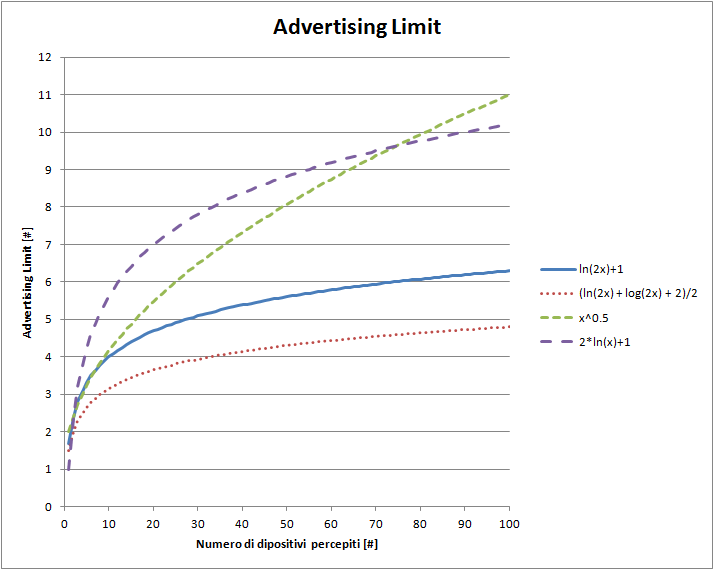
\includegraphics[width=0.9\linewidth]{Images/grafici_usati/AL_curve_no_arr}
	\caption[AL]{Curve di Advertising Limit.}
	\label{fig:AL_curve_no_arr}
\end{figure}

\begin{figure}[t]
	\centering
	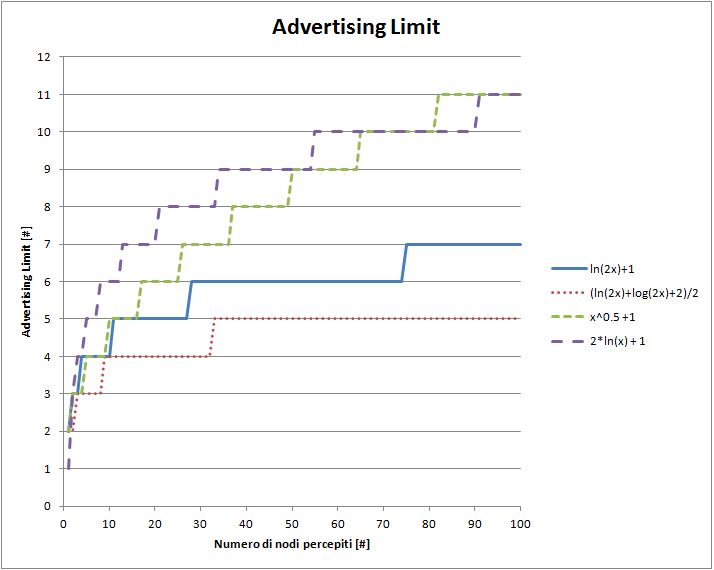
\includegraphics[width=0.9\linewidth]{Images/grafici_usati/AL_curve_arr}
	\caption[AL arrotondato]{Curve di Advertising Limit, arrotondate per eccesso.}
	\label{fig:AL_curve_arr}
\end{figure}

	\chapter{Simulazioni e valutazione risultati}
\label{chap:sim_val}

\section{Organizzazione simulazioni}
La parte di realizzazione sperimentale del nostro progetto, è stata fatta tramite simulazioni con lo scopo di verificare il comportamento del nostro algoritmo e raccogliere dati per fare un'analisi più oggettiva delle sue prestazioni al variare delle condizioni. Per avere una sufficiente base statistica, abbiamo impostato nel file d'inizializzazione il numero di simulazioni a 20. Significa che per ogni configurazione il simulatore eseguirà venti simulazioni consecutive senza reimpostare il generatore di numeri casuali, in questo modo abbiamo ottenuto venti configurazioni di rete differenti per ogni configurazione. Per impostare il numero di ripetizioni da eseguire, abbiamo inserito nella sezione General di ogni file d'inizializzazione utilizzato, l'istruzione “repeat = 20”.

Le simulazioni sono state organizzate rispetto a due parametri principalmente: la densità di nodi e il raggio di trasmissione del BT. Come presentato nella \MySec{sec:modello_rete}, le densità studiate sono:
\begin{itemize}
	\item $d = 0.02 \, \dfrac{nodi}{m^{2}} $.
	\item $d = 0.01 \, \dfrac{nodi}{m^{2}} $.
	\item $d = 0.008 \, \dfrac{nodi}{m^{2}} $.
	\item $d = 0.001 \, \dfrac{nodi}{m^{2}} $.
	\item $d = 0.0005 \, \dfrac{nodi}{m^{2}} $.
	\item $d = 0.0001 \, \dfrac{nodi}{m^{2}} $.
\end{itemize}
E i valori del raggio $\rho$ sono:
\begin{itemize}
	\item $\rho$ = 15 m.
	\item $\rho$ = 50 m.
\end{itemize}
Le densità da $d=0.02\,nodi/m^2$ a $d=0.001\, nodi/m^2$ sono state pensate per simulare ambienti urbani che possono essere dal mediamente popolati al densamente popolati. Situazioni simili sono il caso di medie-grandi città o per le densità più elevate, situazioni di forte concentrazione di persone in un'area ristretta. Quest'ultimo caso può essere generato da una locale alta concentrazione abitativa come una serie di palazzi o condomini vicini tra loro, ma anche da motivazioni esterne come eventi che concentrano molte persone in uno stesso luogo. Le densità più piccole, $d=0.0005\, nodi/m^2$ e $d=0.0001\, nodi/m^2$ sono state pensate per studiare la scalabilità del sistema a fronte della dispersione dei nodi su una vasta area, ma anche per simulare situazioni urbanistiche tipiche di piccoli comuni, con un relativo basso numero di abitanti come ad esempio i piccoli paesi di campagna. Abbiamo quindi organizzato il processo di realizzazione sperimentale in modo da eseguire, per ogni densità, simulazioni per entrambi i raggi $\rho$ e collezionare dati per un'analisi a posteriori delle performance.

Il principale risultato che abbiamo voluto monitorare è stato la percentuale di diffusione dell'informazione al diminuire della densità, per studiare quali fossero i limiti di applicabilità in termini di efficienza del sistema e per avere un insieme di scenari in cui l'algoritmo da noi proposto presentasse buoni livelli di prestazioni. Parallelamente abbiamo anche raccolto dati sul tempo totale di trasmissione, inteso come l'istante di tempo in cui l'ultima trasmissione si è conclusa. Abbiamo scelto di raccogliere anche quest'ultimo dato perché abbiamo cercato di capire quali sono i tempi medi e massimi di diffusione del messaggio. Il motivo è stato di voler dare un corrispettivo valore temporale alla percentuale di nodi che l'algoritmo raggiunge. Da solo un valore di tempo massimo di trasmissione non è valutabile, poiché è molto dipendente dalla dispersione spaziale della rete; per come è costruita la rete non vi è garanzia che tutti i nodi siano connessi ad uno stesso grafo. Per questo motivo, il tempo totale di trasmissione deve essere analizzato in coppia con il valore percentuale di rete coperta durante quella specifica simulazione. In questo modo possiamo avere un'idea di come il tempo di propagazione evolva al variare della copertura e della densità della rete.
\bigskip

\subsection{Algoritmo Dynamic Fanout: funzionamento}
In questa sezione diamo una breve spiegazione sul funzionamento dell'algoritmo all'atto pratico dell'esecuzione. Presenteremo il suo comportamento descrivendo le tre principali configurazioni di lavoro. Faremo riferimento ai diagrammi di flusso in \MyAppendix{apx:diagrammi_fsa} durante la descrizione. Ricordiamo che i diagrammi rappresentano l'elenco di istruzioni della relativa situazione di lavoro. I tre principali momenti di lavoro sono i seguenti: standby, invio di un nuovo messaggio e Ricezione di un messaggio. Vi è anche un'insieme di istruzioni parallelo alle tre configurazioni, che viene eseguito sempre, in maniera periodica.
\bigskip

\noindent{\textbf{\textit{Standby}}}

Partiamo con la situazione di standby e si faccia riferimento al diagramma in \MyAppendix{apx:stb_fsa}. Quando il sistema si trova in una situazione di Standby, vuol dire che in quel momento non è impegnato in nessuna trasmissione nè ricezione. In questa situazione di lavoro il sistema, inizia nello stato di Standby del \acs{BLE}. All'occorrenza dell'esecuzione delle azioni periodiche, vengono eseguiti i rispettivi calcoli periodici e poi viene fatto un controllo se la batteria è sopra la soglia limite del 10\% e se il sistema non sia occupato. Ovviamente essendo in stato di Standby il sistema non è impegnato in nessuna attività e se vi è sufficiente batteria, il sistema passa in stato di Initiating, rimanendo in ascolto e aspettando eventuali comunicazioni sulla rete. Parallelamente, con in maniera ciclica e indipendente, verranno eseguire le azioni periodiche e ogni volta, dopo, verrà fatto il controllo sul livello di batteria. Qualora esso scenda sotto la soglia limite, il sistema verrà portato in stato di Standby e da li non si muoverà finché la batteria non verrà ricaricata. Le azioni periodiche vengono eseguite sempre anche quando il sistema in Standby per monitorare lo stato della rete e della batteria del dispositivo.

Indipendentemente dallo stato in cui il sistema si trova, Standby o Initiating, se il sistema riceve dall'utente il comando di inviare un nuovo messaggio, il dispositivo passa a eseguire le istruzioni della configurazione di invio messaggio. Viene lasciata la possibilità di inviare un messaggio dallo stato di Standby, anche se la batteria è inferiore al 10\%, perché negli scenari di lavoro ipotizzati, potrebbe rivelarsi comunque utile inviare un nuovo messaggio, anche se si potrebbe inficiare sull'autonomia del dispositivo. In tale situazione il sistema invierà solo una volta il messaggio e poi si riporterà da solo in stato di Standby. Nel caso invece il sistema si trovi in stato di Initiating e percepisca un nuovo messaggio sulla rete, si porta in configurazione di ricezione.
\bigskip

\noindent{\textbf{\textit{Azioni periodiche}}}

Sempre in riferimento a \MyAppendix{apx:stb_fsa}, descriviamo cosa trattano le azioni periodiche. Il sistema schedula ad intervalli regolari, un insieme di istruzioni da eseguire chiamate azioni periodiche. Queste azioni sono eseguite sempre, indipendentemente dalla situazione e dalla configurazione in cui il dispositivo sta operando. La periodicità è stata scelta di 30 secondi. Le azioni periodiche servono per aggiornare i parametri utilizzati dall'algoritmo di diffusione (\acs{DF} e \acs{AL}), in modo che dinamicamente si adattino all'ambiente esterno e allo stato attuale del dispositivo stesso. Dopo le operazioni di aggiornamento, viene anche fatto un controllo sul livello della batteria, come descritto per la configurazione di standby. Il controllo riguarda il livello della batteria e se il sistema rileva che la batteria è sopra la soglia limite (10\% come soglia limite), allora non interviene, ma nel caso sia sotto la soglia limite, viene segnalato e se il dispositivo non è impegnato il sistema viene portato in stato di Standby in cui rimarrà finché la batteria non tornerà sopra il 10\%. Questi controlli avvengono anche durante trasmissioni di scambio dati, ma in quel caso il sistema è occupato e si lascia terminare l'operazione, prima di portare il sistema in Standby. Non si vuole che una trasmissione già iniziata venga troncata a causa del controllo, poiché non vogliamo che vada a intralciare il processo di diffusione dell'informazione, ma può comunque agire tra una trasmissione e l'altra. Questo non grava troppo sull'autonomia in quanto il singolo scambio dati, per quanto grossa possa essere l'informazione, non rappresenta una grossa richiesta energetica. Anche quando la batteria è sotto la soglia limite e il sistema è in stato di Standby, i controlli, grazie alla loro esigua richiesta energetica, sono sempre effettuati per riabilitare il sistema al lavoro attivo qualora la batteria venga ricaricata e torni sopra soglia. Una parte dei controlli periodici è già stata inserita e rappresentati nel diagramma di flusso della configurazione di standby, per dare una semplice idea di quale sia il compito di questi controlli, ma non sono vincolati a nessuna configurazione. Esse restano organizzate ed eseguite in maniera indipendente. Per quanto riguarda la sola parte di simulazione, abbiamo inserito nelle azioni periodiche anche il decremento della batteria dei dispositivi, per simulare l'uso del dispositivo da parte dell'utente. Il decremento è piccolo per indicare il consumo medio in idle. Per le trasmissioni completate invece, vi è un decremento più grande dovuto alla grandezza dell'informazione.
\bigskip

\noindent{\textbf{\textit{Invio di un messaggio}}}

Quando è necessario inviare un nuovo messaggio, che esso sia stato ricevuto dalla rete oppure venga inviato dall'utente, il sistema entra in configurazione di invio. Si faccia riferimento al diagramma all'\MyAppendix{apx:invio_fsa}. Appena entrato in questa modalità, il sistema controlla di eseguire una transizione di stato corretta, quindi se non era già in stato di Standby, si porta in stato di Standby. Poi vengono inizializzati i contatori di trasmissioni e di \acs{AE}. A questo punto può entrare in stato di Advertising e iniziare le operazioni per l'invio. Viene incrementato di uno il contatore degli AE e poi il sistema esegue l'\acs{AE} vero e proprio. Durante l'\acs{AE} il sistema trasmette pacchetti di tipo "advertising indiretto" (ADV\_IND \cite{BT-CoreSpec4.0}). Dopo di che si mette in ascolto, aspettando eventuali risposte e viene fatto partire il timeout. Se il timeout scade e nessuna richiesta di connessione è arrivata al dispositivo, esso controlla se il $\textit{AE counter}$ è minore dell'AL. In caso positivo, vuol dire che nessuno è più interessato e quindi viene riportato il sistema in configurazione di standby. In caso negativo invece, il sistema ricomincia tutto il processo di advertising. Nel caso invece che, prima dello scadere del timeout, arrivi una richiesta di connessione (CONN\_REQ \cite{BT-CoreSpec4.0}), il sistema procede a segnalare che è occupato in una trasmissione, così da evitare interruzioni dai controlli di sistema, e poi entra in stato di Connection col ruolo di Slave. Quando il nodo col ruolo di Master invia la richiesta id \textit{pool}, inizia il vero e proprio \acf{CE}, in cui il sistema trasmette al richiedente tutta l'informazione. Al termine del \acs{CE}, viene incrementato il contatore di trasmissioni effettuate, viene decrementato il livello della batteria a causa della trasmissione appena effettuata, il sistema segnala di non essere più occupato, passa in stato di Standby e controlla che se ha raggiunto il limite di trasmissioni imposto dal DF. In caso affermativo, il sistema ha raggiunto la sua quota di lavoro e può tornare in configurazione di standby, mentre in caso contrario, il sistema si riporta in stato di Advertising pronto a ricominciare.
\bigskip

\noindent{\textbf{\textit{Ricezione di un messaggio}}}

Quando il dispositivo rileva che uno o più nodi stanno diffondendo informazioni che il sistema non ha ancora ricevuto, esso entra in configurazione di ricezione di un messaggio, descritto dal diagramma in \MyAppendix{apx:ricevi_fsa}. Questa configurazione è accessibile solo da uno stato di ascolto, ma comunque viene controllato come prima cosa che il sistema sia nel corretto stato. Se non si trova in stato di Initiating, si porta prima in stato di Standby e poi in stato di Initiating. A questo punto il sistema è pronto alla connettersi, quindi risponderà al primo pacchetto di advertising (ADV\_IND \cite{BT-CoreSpec4.0}) che riceve, inviando a sua volta una richiesta di connessione (CONN\_REQ \cite{BT-CoreSpec4.0}). Dopo di che, il sistema si segna occupato e entra in stato di Connection col ruolo di Master. A questo punto invia la sua richiesta di \textit{pool} e lancia il timeout. Il sistema non sa ancora se il dispositivo mittente ha accettato la sua connessione. L'unica cosa che può fare dopo aver inviato la richiesta di pool, è aspettare. Se il timeout scade e non è stata ricevuta nessuna informazione, vuol dire che il mittente non ha accettato la richiesta di connessione oppure era già impegnato in un altra trasmissione. Capendo di non essere stato scelto per la trasmissione, il sistema si dichiara non occupato e si riporta in stato di Initiating in ascolto, pronto a ricominciare. Nel caso invece la richiesta di connessione venga accetta, in risposta alla richiesta di \textit{pool}, inizierà il \acs{CE} e il dispositivo advertiser invierà l'informazione. Una volta terminato il \acs{CE}, viene decrementato il livello della batteria a causa della trasmissione appena effettuata, il sistema si dice non più occupato e si prepara ad entrare in configurazione di invio per diffondere a sua volta l'informazione.
\bigskip

\section{Valutazione risultati}
Dopo aver terminato le simulazioni, abbiamo raccolto i dati ed eseguito analisi su di essi. I parametri che abbiamo monitorato come risultati, a fronte dell'invio di un singolo messaggio sono stati:
\begin{itemize}
	\item Copertura: percentuale di contagio che il messaggio ha raggiunto.
	\item Tempo totale di trasmissione: tempo totale impiegato per raggiungere tale copertura di rete.
\end{itemize}
Grazie alle funzionalità offerte dal framework di simulazione OMNeT++, è stato possibile raccogliere i dati in maniera efficiente. Con una manipolazione dei dati appena raccolti, il framework è stato in grado di fornirci il valor medio, la varianza, la deviazione standard e anche l'intervallo di confidenza al 95\%. Abbiamo anche estratto dai dati raccolti, gli stessi indici tramite un foglio di calcolo Excel, in modo da poter validare ed eventualmente correggere eventuali errori o approssimazioni del software di simulazione.

Prima di parlare dei singoli risultati, ripetiamo alcuni aspetti che hanno caratterizzato l'algoritmo, i modelli e la simulazione stessa. Per avere una maggior variabilità nella simulazione, abbiamo assegnato molti valori di parametri tramite l'uso di generatori casuali, come ad esempio la disposizione dei nodi nella rete, il livello di batteria iniziale di ogni dispositivo e, per ogni ripetizione, la scelta del nodo che possiede l'informazione da divulgare e che inizierà la diffusione. Per ogni densità, sono stati simulati i due range $\rho$ scelti, $\rho=15m$ e $\rho=50m$, e poi è stata fatta la media tra i due. Inoltre la diversità di prestazioni dovuta alla differenza di raggio $\rho$ utilizzato è elevata. Questi aspetti saranno ripresi quando illustreremo i risultati ottenuti.

Il primo parametro che presentiamo è quello della percentuale di rete contagiata dal messaggio, la \textbf{\textit{copertura}}. In \myFig{fig:copertura} sono riportati su grafico i valori medi dei dati raccolti relativi alla copertura raggiunta dal messaggio, per ogni densità simulata. Per ogni curva abbiamo anche riportato sul grafico, il suo intervallo di confidenza al 95\%, per comprendere la distribuzione attorno ai valori medi. La prima cosa che si nota è che per le densità $d=0.02\, nodi/m^2$, $d=0.01\, nodi/m^2$ e $d=0.008\, nodi/m^2$ la percentuale di contagio è intorno al 100\% ed è indicativo di un'ottima efficienza prestazionale della soluzione da noi proposta in ambienti densamente popolati o in momenti di alta concentrazione urbana per motivi particolari. Per queste tre densità molto alte entrambi i raggi $\rho$ hanno dato ottimi valori. Le tre densità più piccole invece hanno evidenziato i limiti di operabilità del sistema. Per la densità $d=0.001\, nodi/m^2$, abbiamo ottenuto ancora degli ottimi valori in termini di copertura, ma in questo caso, il raggio $\rho=15m$ ha cominciato a evidenziare problemi nello stabilire collegamenti tra i nodi e quindi raggiungere un'ottima copertura. Per questo motivo abbiamo ottenuto un intervallo di confidenza già ben più ampio rispetto alle tre casistiche precedenti nelle quali era pressoché nullo o molto piccolo. Nel complesso rimane comunque stabile in un intorno del 90\% al crescere del numero dei nodi nella rete.
\bigskip
\begin{figure}[t]
	\centering
	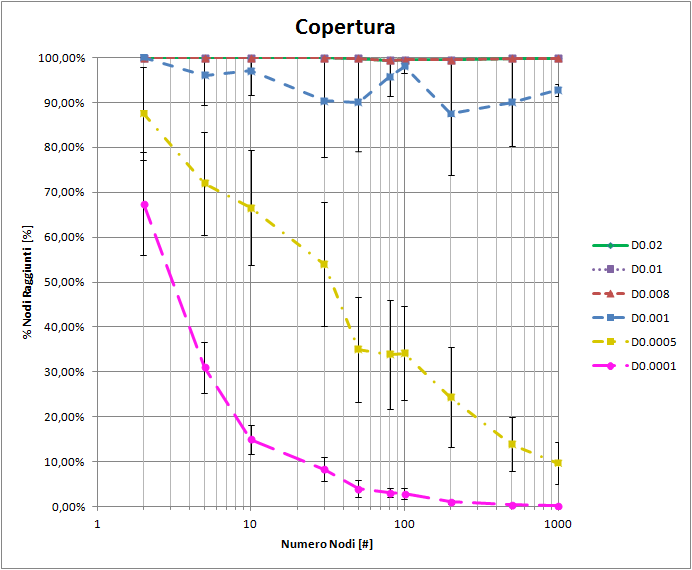
\includegraphics[width=0.9\linewidth]{Images/risultati/copertura}
	\caption[Copertura]{Grafico della copertura della rete.}
	\label{fig:copertura}
\end{figure}

Poi abbiamo la curva della densità $d=0.0005\, nodi/m^2$. Questo valore di densità, rispetto al precedente, presenta un andamento decrescente, al crescere del numero di nodi. Già a questo livello di densità, abbiamo riscontrato che al crescere della rete, aumenta la probabilità che si formino sottoreti isolate che causano solo una diffusione parziale del messaggio. Rispetto alla densità precedente che era il doppio, abbiamo avuto un forte deterioramento nella copertura della rete e un più ampio intervallo di confidenza. Con questo valore di densità, si ha che al crescere del numero di nodi, essi comincino ad essere troppo diradati nella rete e nel complesso si vengano a creare sottoreti sempre più piccole col crescere del numero di nodi. Con le ipotesi fatte, non vi è modo per l'algoritmo di eludere o superare quest'ostacolo. Nonostante quest'andamento decrescente, possiamo vedere che con mille nodi nella rete, il sistema sarebbe in grado di coprire una porzione di rete intorno al 10\%; per questo motivo la densità $d=0.0005\, nodi/m^2$ può essere considerata un limite inferiore di operatività. Infine l'ultima densità $d=0.0001\, nodi/m^2$ si dimostra essere oltre le possibilità operative del sistema, infatti, mostra un degrado prestazionale forte già con reti piccole composte di soli dieci nodi.
Dalle nostre simulazioni è emerso che il sistema è in grado di gestire e operare a livelli ottimi, copertura intorno al 90\% circa, fino a densità $d=0.001\, nodi/m^2$ ma può operare, se pur con un degrado prestazionale linearmente dipendente dalla grandezza della rete, anche fino a una densità minima di $d=0.0005\, nodi/m^2$.

\begin{figure}[t]
	\centering
	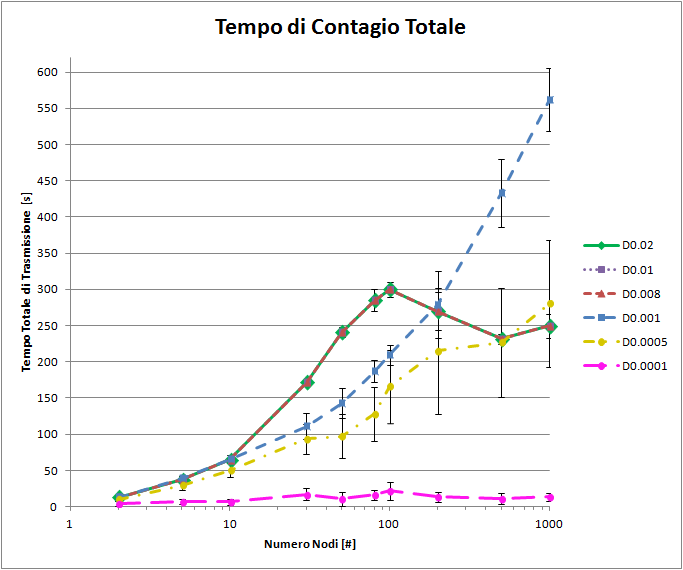
\includegraphics[width=0.9\linewidth]{Images/risultati/tempo_totale}
	\caption[Tempo totale di trasmissione]{Grafico del tempo totale di trasmissione.}
	\label{fig:tempo_totale}
\end{figure}
In \myFig{fig:tempo_totale} riportiamo i risultati riguardanti il \textbf{\textit{tempo totale di trasmissione}}, tempo che l'algoritmo ha impiegato per completare l'ultima trasmissione di contagio a lui possibile. Dalle nostre analisi è risultato che per densità basse come $d=0.02\, nodi/m^2$, $d=0.01\, nodi/m^2$ e $d=0.008\, nodi/m^2$, l'alta vicinanza a permesso di contenere il tempo necessario e dopo un picco in corrispondenza di cento nodi, esso diminuisce pur garantendo una copertura totale o quasi. Questo grazie all'alta ridondanza di collegamenti creatasi dalla vicinanza dei nodi; in questo modo la rete stessa riesce a evitare la formazione di colli di bottiglia tra gruppi di nodi. Per $d=0.001\, nodi/m^2$ invece, abbiamo un andamento crescente col numero di nodi, anche se in \myFig{fig:copertura} si vede come resti sempre vicino alla copertura totale.  In questo caso abbiamo un andamento di tipo quadratico, al crescere del numero di nodi nella rete. Già passando da $d=0.008\, nodi/m^2$ a $d=0.001\, nodi/m^2$ si può notare come cambi il tempo necessario all'algoritmo per raggiungere la sua massima copertura. Infine, le densità d=0.0005 e d=0.0001 presentano curve inferiori alle precedenti ma vanno lette in combinazione con i risultati mostrati in \myFig{fig:copertura}. 
Notiamo che l'andamento, almeno per la curva $d=0.0005\, nodi/m^2$, riamane di tipo quadratico, indice di una rete sempre più diradata nella quale si perdono sempre più i collegamenti ridondanti tra i nodi e compaiono sempre più sottoreti e singoli collegamenti tra essi, che sono il punto debole dell'algoritmo. Se al crescere del numero di nodi, la percentuale di rete coperta diminuisce, significa che il sistema esegue sempre meno trasmissioni, per questa ragione le curve per $d=0.0005\, nodi/m^2$ e $d=0.0001\, nodi/m^2$ sono inferiori alle altre. Per la curva di densità più bassa $d=0.0001\, nodi/m^2$, possiamo solo da dire che conferma i dati rilevati della copertura. L'impossibilità eseguire trasmissioni a causa di una rete troppo sparsa, fa sì che l'algoritmo perda efficacia e si fermi dopo pochi secondi di operatività.

Per valutare meglio l'efficacia della propagazione, abbiamo anche analizzato un \textit{\textbf{fattore di efficienza}}: il rapporto tra la copertura raggiunta, in termini di numero di nodi, e il tempo impiegato per raggiungerla. In \myFig{fig:fattorediefficienza_log} riportiamo i risultati su grafico. Dal grafico si nota come tutte le densità tra $d=0.02\, nodi/m^2$ a $d=0.001\, nodi/m^2$ siano molto simili in termini di efficienza. L'estrema vicinanza tra i nodi per $d=0.02\, nodi/m^2$, rende l'algoritmo molto efficace, ma anche scendendo fino a $d=0.001\, nodi/m^2$ l'efficienza dell'algoritmo rimane buona e l'andamento rimane lo stesso delle densità più alte. Per le due densità limite invece si nota come l'efficienza per la $d=0.0005\, nodi/m^2$ fatichi ad aumentare all'aumentare del numero di nodi, mentre per la $d=0.0001\, nodi/m^2$ si noti come continui a decrescere, fatta eccezione per qualche piccolo picco e per il valore superiore per $n=2$. Quest'ultimo fatto è dovuto a una scelta di progettazione, per agevolare l'analisi dei dati. Quando il primo nodo è inizializzato col messaggio da inviare, il sistema registra il tempo di consegna come l'istante del primo contagio che è sicuramente inferiore al tempo necessario per contagiare l'altro nodo, in una rete formata da due soli nodi. Per questo motivo, per reti piccole risulta avere un'efficienza più alta. All'aumentare della grandezza della rete la curva per $d=0.0001\, nodi/m^2$ si stabilizza e non presenta più il problema, rappresentando il corretto andamento.
\begin{figure}[t]
	\centering
	\includegraphics[width=0.9\linewidth]{"Images/risultati/fattore di efficienza_log"}
	\caption[Fattore di Efficienza]{Grafico del fattore di efficienza}
	\label{fig:fattorediefficienza_log}
\end{figure}

Dopo l'analisi dei dati raccolti, è difficile poter dire con che legge si comporta il nostro algoritmo, per vari motivi. Il primo tra tutti è che non abbiamo sempre una situazione in cui ogni nodo sia connesso in un unico grafo. Le diverse densità possono creare più sottografi isolati senza la possibilità che questi ultimi possano comunicare. Un altro fattore importante è che i nodi del grafo sono dispositivi con una batteria e l'energia a disposizione si consuma nel tempo. Nodi in posizioni critiche della rete possono esaurire la batteria e così escludere parte della rete. Sul fattore batteria sono calibrati i parametri del sistema, e i limiti di trasmissione. Un nodo con limiti di trasmissione bassi, potrebbe completare il suo lavoro di trasmissione, ma verso una zona di rete già abbastanza informata e non in una zona di rete in cui l'informazione non è ancora arrivata. Un altro fattore molto importante e influente, è il metodo (o i metodi) di terminazione che si è scelto di utilizzare. Differenti metodi con differenti criteri possono portare ad avere prestazioni molto differenti.

In condizioni ideali, tutti i nodi connessi in un unico grafo e batteria infinita per tutti i dispositivi, come presentato in \cite{gossip2000-comp} e in \cite{schindel2004-epidemicAlg}, gli algoritmi di rumor mongering con strategia di diffusione push\&pull hanno queste caratteristiche:
\begin{itemize}
	\item L'informazione viene diffusa a tutti dopo $ O\left( \ln \mathit{n} \right)  $ cicli.
	\item La copertura completa richiede almeno $ O\left( \mathit{n}\cdot\log \log \mathit{n} \right)  $ trasmissioni/messaggi.
\end{itemize}
Con \textit{n} il numero di nodi della rete. Per gli algoritmi di rumor mongering di tipo "\textit{address-indipendent}", le complessità appena elencate sono completamente indipendenti dal modo in cui vengono scegli i nodi con cui comunicare e le distribuzioni di probabilità con cui i nodi vengono scelti. Gli algoritmi di tipo "\textit{address-indipendent}" sono algoritmi che, ad ogni iterazione, non dipendono dalla posizione e/o dall'indirizzo dei nodi vicini, ma solo dal numero di nodi vicini. Per questo motivo, questi algoritmi lavorano allo stesso modo sia se hanno una visione completa della rete sia se hanno una visione parziale della rete, l'importante è che siano "\textit{address-indipendent}".

Aspetti che non sono stati considerati in questo studio e che possono avere un impatto sulle prestazioni sono: la mobilità dei nodi e una distribuzione dei nodi nell'area non più totalmente uniforme, ma con una logica più vicina al centro abitativo. Le zone abitative sono costruite vicino ad altre già presenti e non in maniera uniforme su un determinato territorio. La mobilità può creare situazioni riconducibili ai veri contagi epidemici. Un nodo a conoscenza di un'informazione può spostarsi in una zona, anche lontana dal punto di partenza, dove l'informazione sarebbe impossibilitata ad arrivare e iniziarne la diffusione. Questo porterebbe a ridurre i problemi generati dalla bassa densità e dalla conseguente formazione di sottoreti isolate.
	\chapter{Conclusioni e sviluppi futuri}
\label{chap:conclusioni_sviluppiFuturi}

La nostra ricerca si pone nell'ambito dello studio per la riduzione e ottimizzazione del consumo energetico e nell'ambito della comunicazione tra dispositivi mobili.  Il nostro lavoro si è concentrato sullo studio di una possibile soluzione alla mancanza delle comuni reti di comunicazioni, quali reti telefoniche e internet. Come risultato del nostro lavoro abbiamo definito un algoritmo (adattativo) progettato come estensione di un algoritmo di gossip, che sfrutta come canale di trasmissione la tecnologia Bluetooth Low Energy, presente su tutti i più comuni dispositivi mobili in commercio. Il nostro algoritmo sfrutta le caratteristiche del gossip per diffondere informazioni e grazie alla sua capacità di adattamento, cerca sempre di trovare un compromesso nel definire il carico di lavoro del dispositivo tra autonomia ed efficienza. Questo per garantire un buon consumo energetico, e non degradare troppo l'autonomia del dispositivo, e allo stesso tempo offrire un'efficiente azione di gossip. Abbiamo analizzato il sistema per diverse situazioni che tengono conto sia delle densità che della dimensione della popolazione coinvolta.

Possibili sviluppi di questo lavoro consistono nell'includere la mobilità dei nodi, in quanto persone; dispositivi contagiati che si spostano possono incrementare le prestazioni in termini di copertura della rete, proprio come nei casi delle epidemie. Un'altra possibile direzione di ricerca consiste nello studio di possibili modi per sfruttare maggiormente tutta la piconet e quindi poter associare più dispositivi slave per ogni master. Altra possibilità di estensione è lo studio di modelli di reti migliori e metodi più efficienti per simulare la distribuzione abitativa dei paesi; in ogni città, gli abitanti non sono mai distribuiti uniformemente su tutta l'area sotto la giurisdizione comunale. Un'altra possibile direzione è lo studio di eventuali pattern o di modelli più accurati che possano incrementare l'efficienza dell'algoritmo, anche a densità basse. Un'altra direzione è anche lo studio per una miglior gestione dei messaggi, magari con l'inserimento di un \acf{TTL} e politiche di rinvio di messaggi, di cui era già stata fermata la diffusione, al rilevamento di nuovi dispositivi nell'area circostante, analizzando la possibilità di trasformare l'algoritmo da tipo \acs{SIR} a nuovi modelli più elaborati.
	
	%\cleardoublepage\ctparttext{Another informational part preamble text here.}
	%\part{Using this Latex template}
	%\chapter{Practical guide to \enquote{ClassicThesis at DEIB}}
\label{chap:conclusion}
This template is ready to be used when writing a thesis at \myDepartment.
It is a modified version of Classic Thesis by Andr\'e Miede that can be found here \url{http://code.google.com/p/classicthesis/}.

\section{Learn \LaTeX}
\LaTeX\ is a document preparation system and document markup language.
It is widely used for the communication and publication of scientific documents in many fields, including mathematics, physics, computer science, statistics, economics, and political science.

\LaTeX\ users are weird people who care about the ligature between \enquote{f} and \enquote{i} and gets pissed off every time they look at a MS Word document.
Nevertheless, they can explain themselves very well as shown in some beautiful guides for the \LaTeX\ world.
My preferred one for beginners is \enquote{The Not So Short Introduction to \LaTeXe}, which can be found \href{http://www.ctan.org/pkg/lshort}{here}.\footnote{\url{http://www.ctan.org/pkg/lshort}}
For italians I also strongly suggest \enquote{L'arte di scrivere con \LaTeX}, that can be found \href{http://www.lorenzopantieri.net/LaTeX_files/ArteLaTeX.pdf}{here}.\footnote{\url{http://www.lorenzopantieri.net/LaTeX_files/ArteLaTeX.pdf}}
It contains everything needed, however I suggest the reading of chapter 3 for a short introduction. \enquote{ClassicThesis} is another guide of the same author that can be useful, download it \href{http://www.lorenzopantieri.net/LaTeX_files/ClassicThesis.pdf}{here}.\footnote{\url{http://www.lorenzopantieri.net/LaTeX_files/ClassicThesis.pdf}}

\section{Install \LaTeX}
If you don't have already a \LaTeX\ system installed, this section will explain everything you need.
The easiest way to get \LaTeX\ is to install TeXLive, which works on all \acp{OS}.
In \url{https://www.tug.org/texlive/} you find the instructions and the files needed - and also get in touch with minimalism of \TeX users. 

Then you will need an editor: I strongly recommend TeXworks because it's very simple and available on all the platforms.
Also you don't need to install it, it's already included in TeXLive.
The official documentation of TeXworks is available \href{https://docs.google.com/file/d/0B5iVT8Q7W44pMk1WSFRKcDRlMU0/preview}{here};\footnote{\url{https://docs.google.com/file/d/0B5iVT8Q7W44pMk1WSFRKcDRlMU0/preview}}
I strongly recommend the reading of chapter 3.
Alternatevely you can read an italian manual: \href{http://profs.sci.univr.it/~gregorio/introtexworks.pdf}{profs.sci.univr.it/\ldots} (just 13 pages, read it!).\footnote{If you already have a preferred editor, just keep using yours.}

After opening TeXworks, I strongly suggest to set these two additional things:
\begin{itemize}
	\item open Preferences, then go the Composition tab: in the second box there, the \enquote{Process instruments}, push the plus button.
In the window just opened, write \verb!Biber! in the \enquote{Name} field, \verb!biber! in the \enquote{Program} field (lowercase!) and then press the plus button to add the argument \verb!$basename!;
	\item again in the same window, set \enquote{Hide console output} to \enquote{never}.
\end{itemize}

Then just test the installation of the template:
\begin{aenumerate}
	\item go into the template home folder;
	\item open the file \verb!ClassicThesis_DEIB.tex!;
	\item select \verb!pdfLaTeX! from the dropdown menu in the top right of the TeXworks window;
	\item press the rounded green button: it compiles the \verb!.tex! file for the first time and open the resulting \verb!.pdf!;
	\item select \verb!Biber! from the same dropdown menu and press again the green button: this compiles the bibliography, a thing you need to repeat only when you change the file \verb!Bibliography.bib!;
	\item select \verb!pdfLaTeX! again and recompile: this is needed to build indices and crossreferences;
\end{aenumerate}
The above compilation procedure is the standard way to translate the \LaTeX\ code into pdfs.

\section{Online editor}
If the above procedure seems too difficult to you and you have an internet connection always available, you might think to use an online editor. The best choice at the time of writing is \url{http:\\\\sharelatex.com} where you can even find this template after registration to the site by looking for \enquote{Classic Thesis At DEIB}. Your project will be saved on their server but you can also download them. The platform allows up to two authors for free accounts.

There is no need to provide instructions for its use since the website has them. They also have an online \LaTeX guide which is also very useful.

\section{Building blocks}

\subsection{File structure}
The template is organized in multiple file and folders:
\begin{aenumerate}

	\item \verb!ClassicThesis_DEIB.tex! is the main file to be compiled, found in the root folder.
You should just add the source filenames you want to include and any hyphenation you need to explictly specify. 

	\item \verb!classicthesis-config.tex! contains options that can be chosen for this template, like the \verb!draft! one that prints date and time at the bottom of every page.
It contains also the definition for the title, the author and others stuff displayed in the titlepage.
Comments within the file should guide you.\footnote{comments are the rows starting with $\%$.} Take a look at it!

	\item \verb!Bibliography.bib! is the \emph{Bibtex} database: it is a normal textfile where you should put books and articles read;

	\item \verb!Chapters! contains the files for the main chapters of your thesis; this is where you will add the chapters text, as well these very words in line 41 of the file \verb!Conclusion.tex!;

	\item \verb!CodeFiles! contains any code snippet you want to include in your thesis with the environment \verb!listings!; it might be some relevant Matlab or C code, as well as long bash scripts;

	\item \verb!FrontBackmatter! contains various files that are included in the main one to produce abstract, titlepages, acknowledgements, \ldots. 
Follow the instructions below to modify them in order to suits your needs;

	\item \verb!Images! contains the \verb!.pdf! or \verb!.png! versions of the images of the thesis.
A \verb!sources! subfolder is also provided for keeping things well organized.

\end{aenumerate}

To modify abstract, preface, acknowledgements snd acronyms, you need to go into the folder \verb!FrontBackmatter! where you will find the following:
\begin{description}

	\item[Abstract.tex] contains the text displayed as \enquote{abstract} and \enquote{sommario} just after the list of figures, tables, etc. Modify the text and leave the rest.

	\item[Acknowledgments.tex] contains the text put just before the table of contents. Modify the text to suit your needs.

	\item[Acronyms.tex] contains the environment \verb!acronym! with the definition of all the acronyms that will be used within the text. Add your own to the list and put the longest as parameter of the environment.
 
	\item[AutoParts] folder contains things that should work without your intervention. Forget them. 

	\item[Dedication.tex] same usage and structure as \verb!Acknowledgements.tex!.

	\item[Estratto.tex] Politecnico di Milano requires an italian long excerpt of theses written in foreign languages.

	\item[Frontespizio.tex] and \verb!FrontespizioIT.tex! are the cover page in english and italian, respectively. Politecnico di Milano requires the italian version of the english cover, so there it is. Both should work perfectly if you modify section 2 of the file \verb!classicthesis-config.tex!, but you may not like the style so modify them as you prefer.
	
	\item[Preface.tex] same usage and structure as \verb!Acknowledgements.tex!.

	\item[Publication.tex] same usage and structure as \verb!Acknowledgements.tex!, but not included by default. Activate it by uncommenting the relevant line in \verb!ClassicThesis_DEIB.tex!.

	\item[RetroFrontespizio.tex] contains the colophon. In most cases is fine as it already is.
\end{description}

\subsection{Environments}
In addition to common \LaTeX\ environments, this thesis is set to use:
\begin{itemize}

	\graffito{The command graffito is used to put some text here, usefull to underline important things before long paragraphs.}

	\item \verb!\begin{aenumerate}! to produce an \verb!\enumerate! with letters instead of numbers, as in the file list above;

	\item \verb!\blockcquote[][]{}{}! to 	\blockcquote[see][p. 111]{bringhurst:2002}{produce a citation
	with reference to author and page}. If the citation is longer than two rows is indented.
This is provided by the package \verb!csquotes!, which settings are in	\verb!classicthesis-config.tex!.
The package also provides \verb!\enquote{!the citation\verb!}! that produces \enquote{correct citation style} according to the language in use.

	\item \verb!\ac{}! and its variations, defined by package \verb!acronyms!, provide nice handling for acronyms, like \ac{XML}, produced with the code \verb!\ac{XML}!.
List them within the environment \verb!acronym! in the file \verb!FrontBackmatter/Acronyms.tex!.

	\item the so called semi-dynamic referencing for chapter, sections, subsections, appendices, figures, tables and equations. They are a set of commands like \verb!\myChap{label_key}! that produce things like \myChap{chap:aChapter}. There are also capital versions of the commands (\verb!\MyChap{}! produces \MyChap{chap:aChapter}). They need a \verb!\label{name}! anchor next to the referred thing.
	\begin{itemize}
		\item\verb!\myChap! for chapters;
		\item\verb!\mySec! for sections;
		\item\verb!\mySubsec! for subsections;
		\item\verb!\myAppendix! for appendices;
		\item\verb!\myFig! for figures;
		\item\verb!\myTab! for tables;
		\item\verb!\myEq! for equations;
	\end{itemize}

	\item references to bibliography are produced in the usual way with \verb!\cite{bib_key}! \cite{bringhurst:2002} and its variations \verb!\citeauthor{bib_key}!, \verb!\citetitle{bib_key}! and others.

	\item figures are handled usually with the code
	\begin{verbatim}
	\begin{figure}
	\centering
	\includegraphics[width=\columnwidth]{Images/your_image_name.pdf} 
	\caption[Short description]{Long description.}
	\label{fig:a_name}
	\end{figure}
	\end{verbatim}
	which produces things like \myFig{fig:massConstraintFeasibility}. Of course, you need to put the image file \verb!your_image_name.pdf! in folder \verb!Images/!.

	\item tables are produced with
	\begin{verbatim}
	\begin{table}[tb]
	\footnotesize
	\centering
	\begin{tabularx}{0.8\textwidth}{llrcl}
	\toprule
	\tableheadline{l}{Algorithm} &
	\tableheadline{l}{Parameter} &
	\tableheadlineMore{3}{c}{Suggested Values} \\
	\midrule
	\tablefirstcol{l}{Any}
	& \acs{NFE} 		& $10\,000 $ & $ \div $ & $ 200\,000$ \\
	& Population Size 	&  $10 $ & $ \div 	$ & $ 1000$ \\
	\midrule
	\tablefirstcol{l}{\ac{GDE3}}
	& \ac{DE} step size & $0.0 $ & $\div $ & $ 1.0$ \\
	& Crossover rate 	& $0.0$ & $ \div $ & $ 1.0$ \\
	\bottomrule
	\end{tabularx}
	\caption[Short description]{Long description.}
	\label{tab:MOEAandParameters}
	\end{table}
	\end{verbatim}
	which produces \myTab{tab:MOEAandParameters}.
\verb!\myfloatalign!, \verb!\tableheadline{}{}! and its variation \verb!\tableheadlineMore{}{}{}! and \verb!\tablefirstcol{}{}! are used to give a common style to all tables in the document.
They are defined in \verb!classicthesis-config.tex!.\footnote{Also do not forget footnotes, created by \texttt{\textbackslash footnote\{\}}, which should be placed after the punctuation mark.}

	\item equation are produced in classic \LaTeX\ way and they turn out be something like this
	\begin{equation}
	\nabla \mathbf{q_s} = U(x,y) - b_t
	\label{eq:massConservation}
	\end{equation}

\end{itemize}

\begin{figure}
\centering
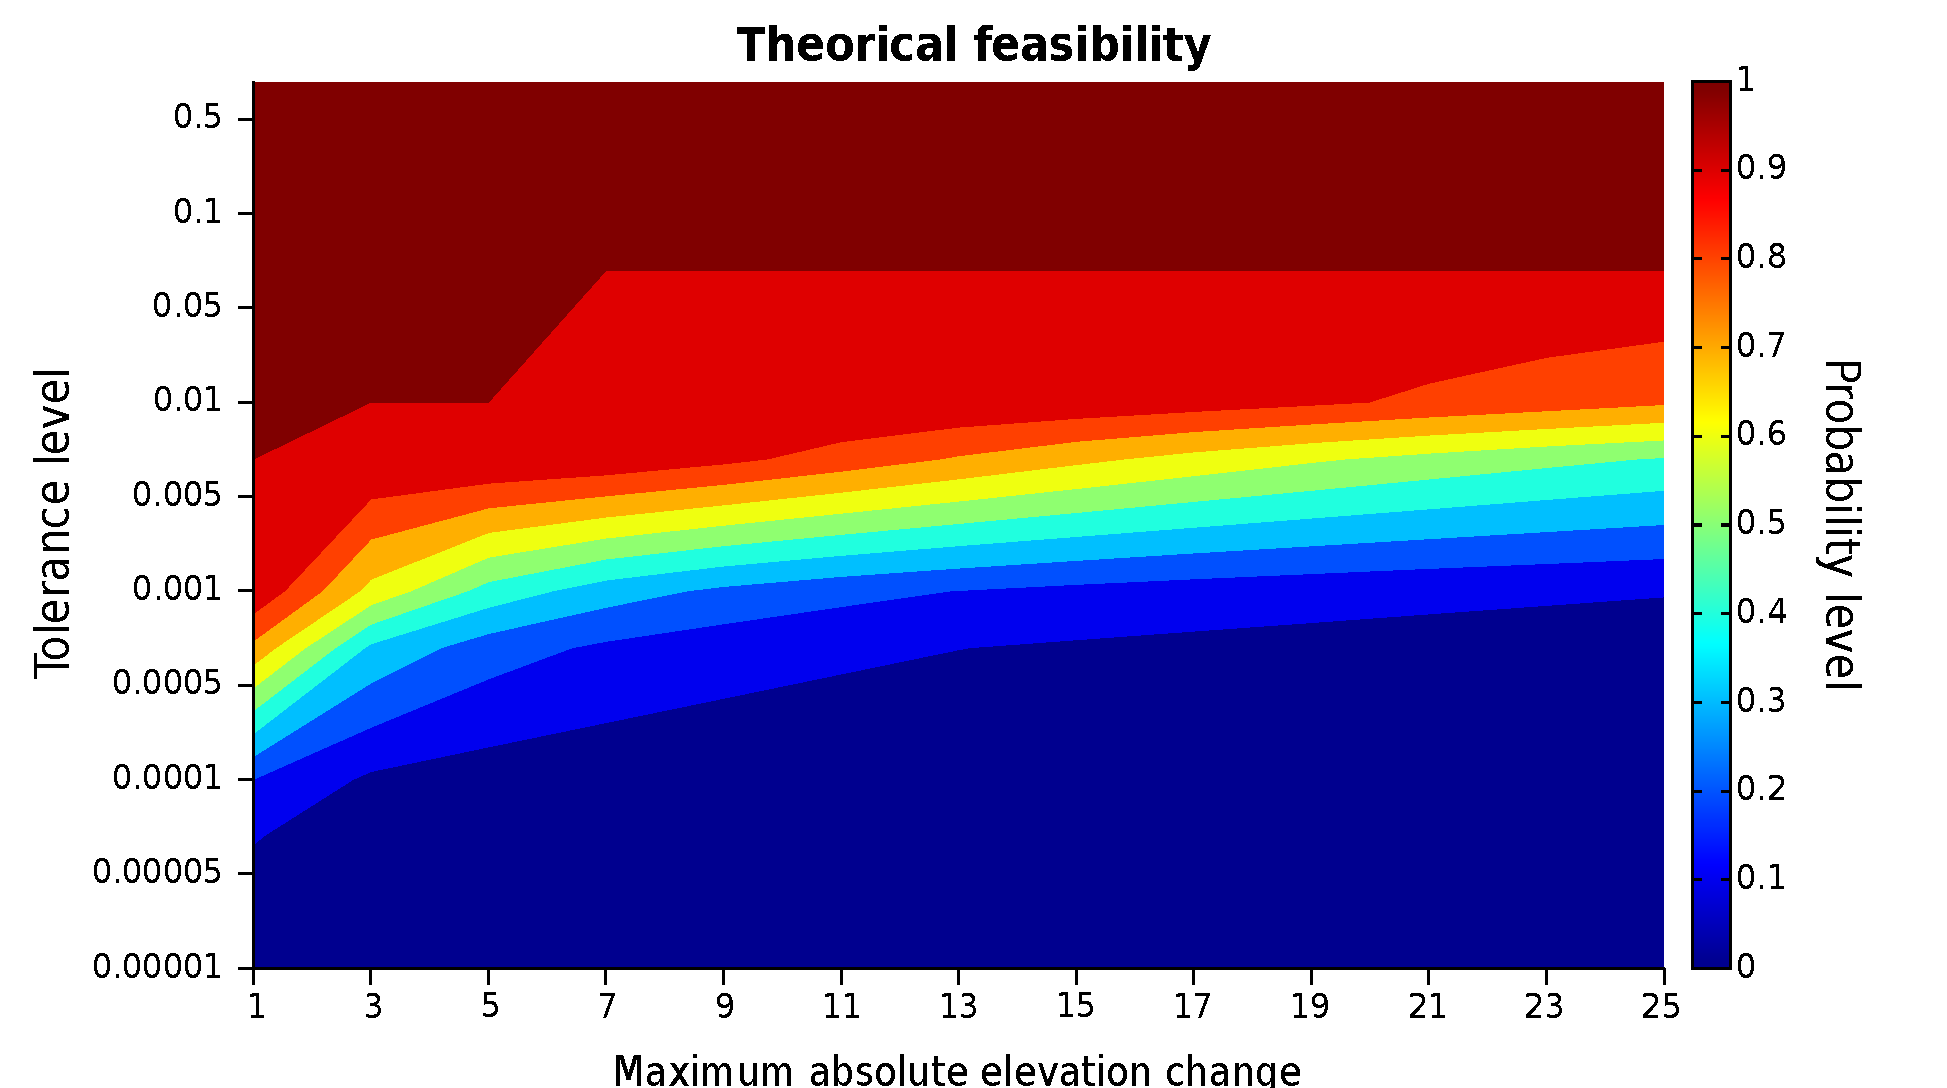
\includegraphics[width=\columnwidth]{Images/feasibilityNR51.pdf}  
\caption[Thing taken from our master thesis]{Thing taken from our master thesis whose meaning have been completely forgotten.}
\label{fig:massConstraintFeasibility}
\end{figure}

\begin{table}
\footnotesize
\centering
\begin{tabularx}{0.8\textwidth}{llrcl}
\toprule
\tableheadline{l}{Algorithm} &
\tableheadline{l}{Parameter} &
\tableheadlineMore{3}{c}{Suggested Values} \\
\midrule
\tablefirstcol{l}{Any}	& NFE	 		& $10\,000 $ 	& $ \div $ 	& $ 200\,000$ \\
				& Population Size 	&  $10 $ 		& $ \div $ 	& $ 1000$ \\
\midrule
\tablefirstcol{l}{GDE3} & DE step size 		& $0.0 $ 	& $\div $ 	& $ 1.0$ \\
				& Crossover rate 	& $0.0$ 	& $ \div $ 	& $ 1.0$ \\
\bottomrule
\end{tabularx}
\caption[Parameters needed for things]{Parameters needed for things that are not needed anymore themselves.}
\label{tab:MOEAandParameters}
\end{table}

\section{Contributing to this template}
Suggestion and improvements are welcome at \url{https://github.com/Lordmzn/ClassicThesis-at-DEIB} or via email at \url{emanuele.mason@polimi.it} or \url{andrea.cominola@polimi.it}.
 
	
	
	% ************************************************************
	% Backmatter
	%*************************************************************
	\cleardoublepage\part{Bibliografia e Appendice}
	\cleardoublepage%********************************************************************
% Bibliography
%*******************************************************
% work-around to have small caps also here in the headline
\manualmark
\markboth{\spacedlowsmallcaps{\bibname}}{\spacedlowsmallcaps{\bibname}}
%\phantomsection 
\stepcounter{dummy} 
% to have the bib a bit from the rest in the toc
\addtocontents{toc}{\protect\vspace{\beforebibskip}}
\addcontentsline{toc}{chapter}{\tocEntry{\bibname}}
\label{app:bibliography}
\printbibliography
	\appendix
	%********************************************************************
% Appendix
%*******************************************************
% If problems with the headers: get headings in appendix etc. right
\markboth{\spacedlowsmallcaps{Appendix}}{\spacedlowsmallcaps{Appendix}}
%************************************************
\chapter{Appendix}

\section{Diagrammi di flusso algoritmo Dyanimc Fanout}
\subsection{Standby FSA}
\label{apx:stb_fsa}
\begin{figure}[h]
	\centering
	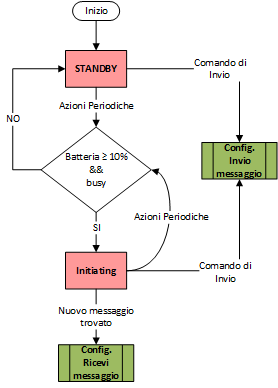
\includegraphics[]{Images/diagrammi_fsa/Standby_fsa}
	\caption[Standby fsa]{Diagramma di flusso della macchina a stati Standby.}
	\label{fig:Standby_fsa}
\end{figure}
\newpage

\subsection{Invia Messaggio FSA}
\label{apx:invio_fsa}
\begin{figure}[!h]
	\centering
	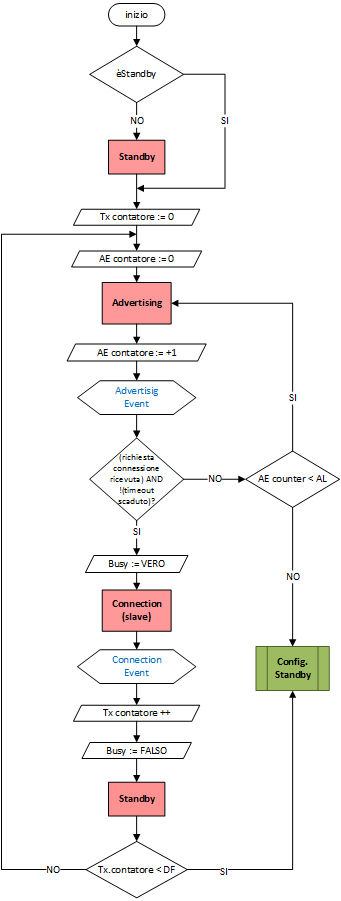
\includegraphics[height= 0.78\textheight]{Images/diagrammi_fsa/Invio_msg_fsa}
	\caption[Invio Messaggio fsa]{Diagramma di flusso della macchina a stati Invio Messaggio.}
	\label{fig:Invio_msg_fsa}
\end{figure}
\newpage
\subsection{Ricevi Messaggio FSA}
\label{apx:ricevi_fsa}
\begin{figure}[!h]
	\centering
	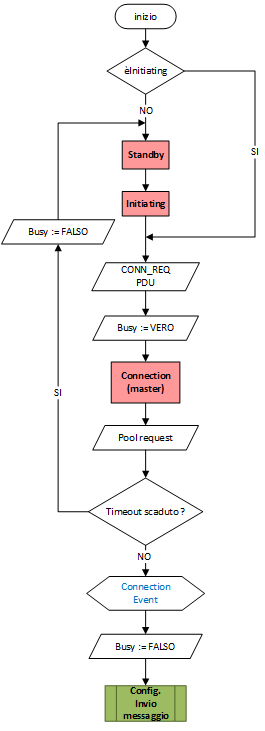
\includegraphics[height= 0.78\textheight]{Images/diagrammi_fsa/Ricevi_msg_fsa}
	\caption[Ricevi Messaggio fsa]{Diagramma di flusso della macchina a stati Ricevi Messaggio.}
	\label{fig:Ricevi_msg_fsa}
\end{figure}


	
\end{document}
% ****************************************************************